
\documentclass[oneside,intlimits,reqno]{scrbook}

%% PACKAGES -------------------------------------------------------------------------------------
\usepackage{array}
\usepackage{enumerate}
\usepackage{mathrsfs}
\usepackage{mathtools}
\usepackage{pgf,tikz}
\usetikzlibrary{arrows}
\usepackage{extarrows}
\usepackage{graphicx,makeidx}
\usepackage{a4wide}
\usepackage{ragged2e}
\usepackage[nottoc]{tocbibind}
\usepackage{amsmath,amssymb,amsthm,amsfonts}
\usepackage{mathabx}
\usepackage[utf8]{inputenc}
\usepackage[czech]{babel}
\usepackage{relsize}
\usepackage[unicode,breaklinks=true,hypertexnames=false]{hyperref}
\def\dotminus{\mathbin{\ooalign{\hss\raise1ex\hbox{.}\hss\cr
			\mathsurround=0pt$-$}}}

%% DEFINICE A REDEFINICE ZÁKLADNÍCH PŘÍKAZŮ ------------------------------------------------------
%definice textu nad rovnítkem
\newcommand{\equal}[1]{\mathop{\overset{#1}{\resizebox{\widthof{.{\ensuremath{\mathop{\overset{#1}{\mathop{=}}}}.}}}{\heightof{=}}{$\mathop{=}$}}}}

% redefinice znaků
\renewcommand{\epsilon}{\varepsilon}
\let\crossedphi\phi
\renewcommand{\phi}{\varphi}
\renewcommand{\rho}{\varrho}
\renewcommand{\emptyset}{\font\cmsy = cmsy10 at 12pt\hbox{\cmsy \char 59}}

% definice českých uvozovek
\def\bq{\mbox{\kern.1ex\protect\raisebox{-1.3ex}[0pt][0pt]{''}\kern-.1ex}}
\def\eq{\mbox{\kern-.1ex``\kern.1ex}}
\gdef\uv#1{\bq #1\eq}

%% MATEMATIKA ----------------------------------------------------------------------------------
% konstanty atd.
\renewcommand{\d}{\mathrm{d}} % diferenciál
\newcommand{\me}{\mathrm{e}} % eulerovo číslo
\newcommand{\mi}{\mathrm{i}} % imaginární jednotka
\newcommand{\LL}{\mathscr{L}}
\newcommand{\Loss}{\mathscr{L}}

% matematické výrazy
\newcommand{\tg}{\mathop{\mathrm{tg}}}				% tangens
\newcommand{\argmin}{\mathop{\mathrm{argmin}}}		% argmin	
\newcommand{\argmax}{\mathop{\mathrm{argmax}}}		% argmax
\newcommand{\argsup}{\mathop{\mathrm{argsup}}}		% argsup
\newcommand{\sgn}{\mathrm{sgn}}						% signum
\renewcommand{\Re}{\mathop{\mathrm{Re}}}
\newcommand{\Ran}{\mathop{\mathrm{Ran}}}
\newcommand{\supp}{\mathop{\mathrm{supp}}}			% support
\renewcommand{\Im}{\mathop{\mathrm{Im}}}
\newcommand{\trace}{\text{tr}} 						% stopa
\newcommand{\inv}[1]{{#1^{-1}}}

% množiny čísel
\newcommand{\R}{\mathbb{R}} % množina reálných čísel
\renewcommand{\C}{\mathbb{C}} % množina komplexních čísel
\newcommand{\Z}{\mathbb{Z}} % množina celých čísel
\newcommand{\N}{\mathbb{N}} % množina přirozených čísel


%% ZKRATKY ---------------------------------------------------------------------------
\newcommand{\MSE}{\mathrm{MSE}}
\newcommand{\MLE}{\mathrm{MLE}}
\newcommand{\LSE}{\mathrm{LSE}}
\newcommand{\MSR}{\mathrm{MSR}}
\newcommand{\NF}{\mathrm{F}}
\newcommand{\A}{\mathrm{A}}
\newcommand{\RMR}{\mathrm{R}}
\newcommand{\SST}{\mathrm{SST}}
\newcommand{\SSE}{\mathrm{SSE}}
\newcommand{\SSR}{\mathrm{SSR}}


% MATICE ------------------------------------------------------------------------------
 % indentita
\newcommand{\I}{\mathbb{I}} % identita
\newcommand{\Identita}[1]{\mathbb{I}_{#1}} % identita s indexem velikosti
% obecné matice A,B,H
\newcommand{\Am}{\mathbb{A}} % matice A
\newcommand{\Bm}{\mathbb{B}}
\newcommand{\Hm}{\mathbb{H}}
\newcommand{\Mm}{\mathbb{M}}
\newcommand{\Wm}{\mathbb{W}}
\newcommand{\Km}{\mathbb{K}}
% Fisherova matice
\newcommand{\fisher}{\mathbb{I}} % Fisherova matice





\newcommand{\Cc}{\mathcal{C}} % funkce třídy C (spojité)
\newcommand{\RR}{\mathcal{R}}



% VEKTORY ----------------------------------------------------------------------------------------------
% vektorová písmenka x,y,X,Y atd.
% tučné X
\newcommand{\X}{\textbf{X}} % klasické
\newcommand{\lX}{\overline{\textbf{X}}} % s pruhem
% tučné Y
\newcommand{\Y}{\textbf{Y}} % klasické
\newcommand{\lY}{\overline{Y}} % s pruhem
% tučné x
\newcommand{\x}{\textbf{x}}
% tučné y
\newcommand{\y}{\textbf{y}}
% tučné z
\newcommand{\z}{\textbf{z}}

% beta
\newcommand{\betab}{\boldsymbol{\beta}} 			% vektorové beta
\newcommand{\bbeta}{\boldsymbol{\beta}}				% také vektorové beta
\newcommand{\wbetab}{\widehat{\boldsymbol{\beta}}}	% vektorové beta se stříškou
% rezidua: e
\newcommand{\eb}{\textbf{e}}
\newcommand{\lei}{\overline{e}_i}
\newcommand{\hei}{\widehat{e}_i}
% epsilon
\newcommand{\epsb}{\boldsymbol{\epsilon}}


%% PROMĚNNÉ SE STŘÍŠKOU -----------------------------------------------------------------------------------
% řecká abeceda
\newcommand{\walpha}{\widehat{\alpha}}				% alpha se stříškou
\newcommand{\wbeta}{\widehat{\beta}}				% beta se stříškou
\newcommand{\wgamma}{\widehat{\gamma}}				% gamma se stříškou
\newcommand{\wsigma}{\widehat{\sigma}}				% sigma se stříškou
\newcommand{\heps}{\widehat{\epsilon}}				% epsilon se stříškou
\newcommand{\hrho}{\widehat{\rho}}
\newcommand{\wtheta}{\widehat{\theta}}
% x se stříškou
\newcommand{\hxn}{\widehat{x}_n}	% xn se stříškou
% y se stříškou
% klasické
\newcommand{\hy}{\widehat{y}}
\newcommand{\hY}{\widehat{Y}}
% z se stříškou
\newcommand{\hz}{\widehat{z}}
\newcommand{\hzb}{\widehat{\z}}
% s indexy
\newcommand{\hyn}{\widehat{y}_n}
\newcommand{\hyi}{\widehat{y}_i}
\newcommand{\hYn}{\widehat{Y}_n}
\newcommand{\hYi}{\widehat{Y}_i}
% vektorové
\newcommand{\hYb}{\widehat{\textbf{Y}}}
\newcommand{\hyb}{\widehat{\textbf{y}}}
% rezidua: e
\newcommand{\he}{\widehat{e}}
\newcommand{\heb}{\widehat{\textbf{e}}}
% a nějaké další
\newcommand{\hsn}{\widehat{\sigma}_n^2}				% sn se stříškou


%% PROMĚNNÉ S PRUHEM --------------------------------------------------------------------------------------
\newcommand{\overbar}[1]{\mkern 1mu\overline{\mkern-1mu#1\mkern-3mu}\mkern 3mu}
\newcommand{\Oxn}{\overbar{\rule{0ex}{1.8ex}X_n}}
\newcommand{\Oyn}{\overbar{\rule{0ex}{1.8ex}Y_n}}
\newcommand{\Ox}[1]{\overbar{\rule{0ex}{1.8ex}X_{#1}}}
\newcommand{\Oy}[1]{\overbar{\rule{0ex}{1.8ex}Y_{#1}}}
\newcommand{\oxn}{\overbar{\rule{0ex}{1.33ex}X_n}}
\newcommand{\ox}[1]{\overbar{\rule{0ex}{1.33ex}X_{#1}}}
\newcommand{\oy}[1]{\overbar{\rule{0ex}{1.33ex}Y_{#1}}}
\newcommand{\oyn}{\overbar{\rule{0ex}{1.33ex}Y_n}}
\newcommand{\omn}{\overbar{\rule{0ex}{1.3ex}\mu_n}}
\newcommand{\oxnn}{\overbar{\rule{0ex}{1.33ex}x_n}}
\newcommand{\oynn}{\overbar{\rule{0ex}{1.33ex}y_n}}

% další možnost
\newcommand{\lyn}{\overline{y}_n}
\newcommand{\ly}{\overline{y}}
\newcommand{\lhyn}{\overline{\hy}_n}
\newcommand{\lhy}{\overline{\hy}}
\newcommand{\lyi}{\overline{y}_i}
\newcommand{\lxn}{\overline{x}_n}
\newcommand{\lx}{\overline{x}}


%% PRAVDĚPODOBNOST ------------------------------------------------------------------------------
% distribuční funkce
\newcommand{\FF}{\mathrm{F}}
\newcommand{\FEX}{\FF_\X}

% hustota pravděpodobnosti
\newcommand{\fex}{f_\X}

% pravděpodobnost
\newcommand{\PP}{\mathbb{P}}
\newcommand{\PEX}{\PP^\X}

% pravděpodobnostní prostor
\newcommand{\prostor}{(\Omega,\mathcal{A},\PP)} 

% charakteristiky
\newcommand{\E}{\mathbb{E}} % střední hodnota
\newcommand{\D}{\mathrm{D}} %  rozptyl
\newcommand{\Cov}{\mathbb{C}\mathrm{ov}} % kovariance

% rozdělení
\newcommand{\NN}{\mathcal{N}} % normální
\newcommand{\AN}{\mathcal{AN}} % asymptoticky normální
\newcommand{\Exp}{\mathrm{Exp}} % exponenciální
\newcommand{\Be}{\mathrm{Be}} % bernoulliho
\newcommand{\Bi}{\mathrm{Bi}} % binomické

% konvergence
\newcommand{\sj}{\stackrel{s.j.}{\longrightarrow}}
\newcommand{\Pto}{\stackrel{\PP}{\to}}
\newcommand{\wto}{\stackrel{w}{\to}}
\newcommand{\Dto}{\stackrel{\mathscr{D}}{\to}}
\newcommand{\PSJ}{\stackrel{\PP,s.j.}{\longrightarrow}}
\newcommand{\Lto}{\stackrel{(\mathscr{L})}{\to}}
\newcommand{\sjP}{\stackrel{s.j.~\PP}{\longrightarrow}}
\newcommand{\Lp}{\stackrel{L_p}{\longrightarrow}}

% pár dalších...
\newcommand{\Aa}{\mathcal{A}}
\newcommand{\Bb}{\mathcal{B}}
\renewcommand{\t}{\theta} % theta
\newcommand{\bmu}{\boldsymbol{\mu}} % vektorové mí

\newcommand{\htm}{\widehat{\t}_\txt{M}}
\newcommand{\html}{\widehat{\t}_\txt{ML}}
\newcommand{\htn}{\widehat{\t}_n}
\newcommand{\rhn}{R_{H_0}}
\newcommand{\Phiast}{\crossedphi^\ast}
\newcommand{\rhno}{\overline{R}_{H_0}}
\newcommand{\freg}{\mathcal{F}_{reg}}
\newcommand{\fregp}{\mathcal{F}_{reg}^+}
\newcommand{\fregml}{\mathcal{F}_{reg}^\txt{ML}}
\newcommand{\RE}{\mathrm{RE}_{2,1}}
\newcommand{\ARE}{\mathrm{ARE}_{2,1}}

% proměnné s dolním složitějším indexem
\newcommand{\hii}{h_{ii}}
\newcommand{\Sxx}{ S_{xx} }

% co moc nikam nepatří...
\newcommand{\core}{\inv{(\textbf{X}^T\textbf{X})}}
\newcommand{\lomn}[1]{\frac{#1}{n}}
\newcommand{\lm}{\frac{1}{m}}
\newcommand{\jednab}{\mathbf{1}}
\newcommand{\norm}[1]{\| #1 \|}
\newcommand{\In}{\mathrm{I}_n}
\newcommand{\Q}{\textbf{Q}}



%% POSLOUPNOSTI, SUMY ATD. -------------------------------------------------------------------------------------
%posloupnosti
\newcommand{\posl}{(X_j)_{j=1}^{+\infty}}
\newcommand{\poslkon}{(X_j)_{j=1}^{n}}
\newcommand{\posln}{(X_n)_{n=1}^{+\infty}}
\newcommand{\poslnn}{(\X_n)_{n=1}^{+\infty}}

%sumy
\newcommand{\suminftyo}{\sum\limits_{n=0}^{+\infty}}
\newcommand{\suminfty}{\sum\limits_{n=1}^{+\infty}}
\newcommand{\sumainfty}[1]{\sum\limits_{#1}^{+\infty}}
\newcommand{\suminftylo}{\sum\limits_{l=0}^{+\infty}}
\newcommand{\sumin}{\sum\limits_{i=1}^{n}}
\newcommand{\sumjn}{\sum\limits_{j=1}^{n}}
\newcommand{\sumjm}{\sum_{j=1}^{m}}
\newcommand{\sm}[2]{\sum\limits_{ #1 }^{ #2 }}


%% NĚJAKÉ DALŠÍ PŘÍKAZY -----------------------------------------------------------------------------------------
\newcommand{\dom}[1]{\mathop{\mathrm{Dom} (#1)}} % definiční obor
\newcommand{\mat}[1]{\mathbf #1}
\newcommand{\abs}[1]{\left|#1\right|}
\renewcommand{\b}[1]{\left( #1 \right)}
\newcommand{\nor}[1]{\left\|#1\right\|}
\newcommand{\Br}[1]{\Bigl(#1\Bigr)}
\newcommand{\br}[1]{\bigl(#1\bigr)}
\newcommand{\e}[1]{\me^{#1}}
\newcommand{\mini}[1]{{#1_{(-1)}}}
\newcommand{\ini}{\theta\in\Theta}
\newcommand{\init}[1]{\theta\in\Theta\subset\R^#1}
\newcommand{\txt}[1]{\mathrm{{\footnotesize  #1 }}}
\newcommand{\matice}[4]{\left(\begin{array}{cc}	#1 & #2 \\ #3 & #4	\end{array} \right)}
\newcommand{\maticehrana}[4]{\left[\begin{array}{cc}	#1 & #2 \\ #3 & #4	\end{array} \right]}
\newcommand{\vektor}[2]{\left(\begin{array}{c}	#1  \\  #2	\end{array} \right)}
\newcommand{\p}[1]{\PP\left( #1 \right)}
\newcommand{\EE}[1]{\E\left[ #1 \right]}
\newcommand{\n}[1]{\NN\left( #1 \right)}
\newcommand{\hypothesis}[2]{H_0: #1 ~\text{vs.}~ H_1: #2 }
\newcommand{\hypothesiswide}[2]{H_0: #1 \qquad\text{vs.}\qquad H_1: #2 }
\newcommand{\silofunkce}[1]{\beta_\crossedphi\big|_{\Theta_{#1}}}
\newcommand{\silofunkceast}[1]{\beta_{\Phiast}\big|_{\Theta_{#1}}}
\newcommand{\hypothesisap}[2]{H'_0: #1 ~\text{vs.}~H'_1: #2 }
\newcommand{\test}[1]{\boxed{\text{TEST: $H_0$ zamítáme, pokud } #1 .}}
\renewcommand{\S}{\mathbb{S}}


%% PROSTŘEDÍ -----------------------------------------------------------------------------------------------------
\theoremstyle{definition}
\newtheorem{define}{Definice}[chapter]
\theoremstyle{plain}
\newtheorem{theorem}[define]{Věta}
\newtheorem{lemma}[define]{Lemma}
\newtheorem{dusl}[define]{Důsledek}
\newtheorem{corollary}[define]{Tvrzení}
\renewcommand{\proofname}{Důkaz}

\theoremstyle{remark}
\newtheorem{example}[define]{\textsc{Příklad}}
\newtheorem{remark}[define]{\textsc{Poznámka}}

\renewcommand{\indexname}{Rejstřík}

\frenchspacing
\setlength{\parindent}{0pt}
\setlength{\parskip}{1pt}

\hypersetup{
 	pdftitle={01RAD - Regresní analýza dat},
 	pdfauthor={WIKI Skripta},
 	pdfsubject={Zápisky z přednášek RAD, FJFI ČVUT},
 	pdfkeywords={regresní analýza dat},
 	bookmarksnumbered=true,
 	colorlinks=true,
 	pdfpagemode={UseOutlines}
 }
\makeindex

\title{01RAD}
\date{\today}
\author{doc.~Ing.~Tomáš Hobza,~Ph.D., Bc. Martin Kovanda,\\ Bc. Michaela Mašková, Bc. Filip Bár}

\begin{document}

% ****************************************************************************************************************************
%                             FRONTMATTER
% ****************************************************************************************************************************
\frontmatter
\maketitle

\newpage
\pdfbookmark[0]{Obsah}{obsah}
\tableofcontents

%\wikiskriptum{01DIFRnew}
% ****************************************************************************************************************************
%                             KAPITOLA: Předmluva
% ****************************************************************************************************************************
\chapter*{Předmluva}
\pdfbookmark[0]{Předmluva}{predmluva}

Materiál byl sestaven na základě poznámek doc. Ing. Tomáše Hobzy, Ph.D., kterému bychom tímto chtěli poděkovat za rozsáhlou korekci vzniklého materiálu. Zmíněné přednášky proběhly v~zimním semestru akademického roku 2020/2021 na~Fakultě jaderné a
fyzikálně inženýrské ČVUT v~Praze. Přednášky nebyly uskutečněny prezenční formou vzhledem k probíhající pandemii Covid-19. 

Tento učební text je určen posluchačům 1.~ročníku navazujícího magisterského studia navštěvujícím kurs 01RAD\emph{	Regresní analýza dat}, který je zařazen
mezi předměty oborů AMSM. Při sestavování textu se předpokládaly znalosti základů matematiky na úrovni absolvování kurzů 01MAB2-4, 01LAB1-2 a 01MIP.

~

\textbf{Doporučená literatura:}
\begin{enumerate}[(1)]
  \item ...
\end{enumerate}



% ****************************************************************************************************************************
%                             MAINMATTER
% ****************************************************************************************************************************
\mainmatter
%%regresní analýza
\chapter{Opakování ze SME}
\section{Jednorozměrná lineární regrese}
%příklad matlab
Předpokládejme, že se~sledují dvě fyzikální veličiny $X$ a~$Y$ mezi~kterými existuje lineární závislost
$$Y=\beta_0+\beta_1X .$$
$\beta_0$ a~$\beta_1$ nejsou známy, a~proto se~provádí experiment, při~němž se~zjišťují hodnoty dvojic $(X,Y)$. Často se~stává, že měření hodnot $X$ probíhá prakticky zcela přesně (například $X$ se~nastavuje na~předem dané úrovně), zatímco $Y$ se~měří s~určitou chybou. Zavádí se~tedy model
$$Y_i=\beta_0 +\beta_1X_i + e_i \quad \forall~i=1,...,n,$$
kde $e_i$ je náhodný šum a~$e_1,...,e_n$ jsou $iid~\NN(0,{\sigma}^2)$ a~dvojice $(x_1,y_1),...,(x_n,y_n)$ získáme měřením. Neznáme parametry jsou $\beta_0,\beta_1, {\sigma}^2$, chtěli bychom je odhadnout na~základě výběru (MLE odhady).\\

Rozdělení $Y_i$ je $Y_i\sim\NN(\beta_0 + \beta_1x,{\sigma}^2)$, a~tedy věrohodnostní funkce výběru $y_1,...,y_n$ je
$$L=\Br{\frac{1}{\sqrt{2\pi{\sigma}^2}}}^n \e{-\frac{1}{2{\sigma}^2}\sum_{i=1}^{n}(Y_i-\beta_0-\beta_1x)^2}.$$
$$l=\ln L=-\frac{n}{2}\ln{2\pi}-\frac{n}{2}\ln{{\sigma}^2}-\frac{1}{2{\sigma}^2}\sum_{i=1}^{n}(Y_i-\beta_0-\beta_1x_i)^2.$$
Je zřejmé, že pro~libovolné ${\sigma}^2$ potřebujeme minimalizovat
$$S(\beta_0,\beta_1)=\sum_{i=1}^{n}(Y_i-\beta_0-\beta_1x_i)^2   $$
přes $\beta_0,\beta_1$, na~což použijeme metodu nejmenších čtverců (poznámka?).
$$\frac{\partial l}{\partial \beta_0}=2\frac{1}{2{\sigma}^2}\sum_{i=1}^{n}(Y_i-\beta_0-\beta_1x_i)=0,  $$
$$\frac{\partial l}{\partial \beta_1}=\frac{1}{{\sigma}^2}\sum_{i=1}^{n}(Y_i-\beta_0-\beta_1x_i) x_i=0. $$
Z toho pak
$$  \sum_{i=1}^{n} Y_i -n\beta_0-\beta_1 \sum_{i=1}^{n} x_i=0, $$
$$ \beta_0=\Oyn -\beta_1\oxnn=\frac{1}{n}\sum_{i=1}^{n}Y_i-\beta_1\frac{1}{n}\sum_{i=1}^{n}x_i.$$
Po vynásobení poslední rovnice $n$ úpravou dostaneme vztah
$$\sum_{i=1}^{n}(Y_i-\Oyn+\beta_1\oxnn-\beta_1x_i)x_i=0  $$
a následně i~vztah
$$ \sum_{i=1}^{n}Y_ix_i-\Oyn\sum_{i=1}^{n}+\beta_1\oxnn\sum_{i=1}^{n}x_i-\beta_1\sum_{i=1}^{n}x_i^2=0. $$
Z toho už následně vyjádříme
$$ \widehat{\beta}_1=\frac{\sum_{i=1}^{n}x_iY_i-n\Oyn\oxnn}{\sum_{i=1}^{n}x_i^2-n\oxnn^2}\qquad\text{a}\qquad \widehat{\beta}_0=\Oyn-\widehat{\beta}_1\oxnn. $$
Nyní již spočítáme logaritmickou věrohodnostní funkci
$$\frac{\partial l}{\partial ({\sigma}^2)}=-\frac{n}{2}\frac{1}{{\sigma}^2}+\frac{1}{2({\sigma}^2)^2}\sum_{i=1}^{n}(Y_i-\beta_0-\beta_1x_i)^2=0,$$
odkud
$$\hsn=\frac{1}{n}\sum_{i=1}^{n}(Y_i-\widehat{\beta}_0-\widehat{\beta}_1x_i)^2. $$
Pokud dále označíme
$$\widehat{Y}_i=\widehat{\beta}_0+\widehat{\beta}_1x_i, $$
pak rozdíly
$$r_i=Y_i-\widehat{Y}_i $$
nazýváme \textbf{rezidua} (která by měla mít normální rozdělení, aby byly splněny předpoklady modelu) a~
$$ \sum_{i=1}^{n}r_i^2=\sum_{i=1}^{n}(Y_i-\widehat{\beta}_0-\widehat{\beta}_1x_i)^2=S_e  $$
nazveme \textbf{reziduální součet čtverců}.
\subsection*{$R^2$ statistika}
Tuto statistiku definujeme vztahem
$$R^2=1-\frac{\sum_{i=1}^{n}r_i^2}{\sum_{i=1}^{n}(Y_i-\oyn)^2}=1-\frac{\sum_{i=1}^{n}(Y_i-\widehat{Y}_i)^2}{\sum_{i=1}^{n}(Y_i-\oyn)^2}, $$
který se~dá chápat jako podíl součtu reziduálních čtverců a~rozptylu $Y$.
$R^2$ se~interpretuje jako poměr variability v~datech vysvětlené lineárním modelem. Čím větší je $R^2$, tím lépe vysvětluje náš model data, v~ideálním případě pak $R^2=1$.
Dále bychom chtěli:
\begin{enumerate}
\item sestrojit IS pro~parametry modelu $\beta_0, \beta_1, {\sigma}^2$,

\item intervaly pro~predikci hodnoty $y$ v~daném bodě $x$ a

\item testovat hypotézy na~parametrech modelu, například F-stat. v~MATLABu testuje $H_0:\beta_0=0$ a~$\beta_1=0$, že vysvětlující proměnná $y$ není korelovaná s~vysvětlovanou proměnnou $x$.
\end{enumerate}


Vše je podobné testům o~parametrech $N(\mu,{\sigma}^2)$ (t-test, F-test), potřebujeme rozdělení odhadů $\widehat{\beta}_0,\widehat{\beta}_1, \widehat{{\sigma}^2}$. Sdružené rozdělení $\widehat{\beta}_0,\widehat{\beta}_1$ se~najde snadno, protože to jsou lineární funkce $Y_i$ takže budou mít normální rozdělení, stačí tedy určit střední hodnoty, rozptyly, kovariance,...\\
Označme výběrový rozptyl $x$ jako
$${\sigma_x}^2=\frac{1}{n}\sum_{i=1}^{n}x_i^2-\oxnn^2. $$
Platí, že
\begin{enumerate}
\item $$ \widehat{\beta}_1\sim \n{\beta_1,\frac{{\sigma}^2}{n{\sigma_x}^2}}, $$
$$\widehat{\beta}_0\sim \n{\beta_0,{\sigma}^2\Br{\frac{1}{n}+\frac{(\oxnn)^2}{n{\sigma_x}^2}}}=\n{\beta_0,\frac{{\sigma}^2}{n{\sigma_x}^2}\frac{1}{n}\sum_{i=1}^{n}x_i^2}, $$
$$\Cov(\widehat{\beta}_0,\widehat{\beta}_1)=-\frac{\oxnn{\sigma}^2}{n{\sigma_x}^2}, $$
\item $\widehat{\sigma}^2 $ je nezávislé na~$\widehat{\beta}_0$ a~$\widehat{\beta}_1$,
\item $$\frac{n\widehat{\sigma}^2}{\sigma^2} \sim {\chi}^2(n-2).$$
\end{enumerate}
%

\begin{remark}
První bod znamená, že $(\beta_0,\beta_1)\sim \NN(\mu,\sum)$, kde
$$\bmu=(\beta_0,\beta_1)\quad \text{a}\quad \sum=\frac{\sigma^2}{n\sigma_x^2}\begin{pmatrix}
\oxnn^2 & -\oxnn\\
-\oxnn & 1
\end{pmatrix}. $$
%\mu vektorově
\end{remark}


Konfidenční intervaly\\
\begin{enumerate}
\item $\sigma^2$, a~protože $\frac{n\widehat{\sigma}^2}{\sigma^2}\sim {\chi}^2(n-2)$, víme, že s~pravděpodobností $\PP=1-\alpha$ bude
$${\chi}^2_{\frac{\alpha}{2}}(n-2) \leq \frac{n\widehat{\sigma}^2}{\sigma^2} \leq {\chi}^2_{1-\frac{\alpha}{2}}(n-2),$$
a tedy $(1-\alpha)$\% IS (interval spolehlivosti) pro~$\sigma^2$ je
$$\frac{n\widehat{\sigma}^2}{{\chi}^2_{1-\frac{\alpha}{2}}(n-2)} \leq \sigma^2 \leq \frac{n\widehat{\sigma}^2}{{\chi}^2_{\frac{\alpha}{2}}(n-2)}.$$
\item $\beta_1$\\
Veličiny 
$\frac{\widehat{\beta}_1-\beta_1}{\sqrt{\frac{\sigma^2}{n\sigma_x^2}}}\sim \NN(0,1) $
a
$\frac{n\widehat{\sigma}^2}{\sigma^2} \sim {\chi}^2(n-2) $
jsou nezávislé. Z~toho vyplývá, že 
$$
 \frac{(\widehat{\beta}_1-\beta_1)\Big/\sqrt{\frac{\sigma^2}{n\sigma_x^2}}}{\sqrt{\frac{n\widehat{\sigma}^2}{\sigma^2}\frac{1}{n-2}}} \sim t(n-2).$$

Z toho potom
\begin{align}
 \frac{\widehat{\beta}_1-\beta_1}{\sqrt{\frac{\widehat{\sigma}^2}{(n-2)\sigma_x^2}}}=(\widehat{\beta}_1-\beta_1)\sqrt{\frac{(n-2)\sigma_x^2}{\widehat{\sigma}^2}}\sim t(n-2), \label{eq1}
\end{align}
což znamená, že
$$-t_{1-\frac{\alpha}{2}}(n-2) \leq (\widehat{\beta}_1-\beta_1)\sqrt{\frac{(n-2)\sigma_x^2}{\widehat{\sigma}^2}}   \leq t_{1-\frac{\alpha}{2}}(n-2)$$
s pravděpodobností $\PP=1-\alpha$, a~tedy
$$\widehat{\beta}_1-t_{1-\frac{\alpha}{2}}(n-2)\sqrt{\frac{\widehat{\sigma}^2}{(n-2)\sigma_x^2}}  \leq \beta_1 \leq \widehat{\beta}_1+t_{1-\frac{\alpha}{2}}(n-2)\sqrt{\frac{\widehat{\sigma}^2}{(n-2)\sigma_x^2}}$$
je $100(1-\alpha)$\% IS pro~$\beta_1$.
Podobně pro~$\beta_0$ dostaneme, že 
$$ \frac{\widehat{\beta}_0-\beta_0}{\sqrt{\sigma^2(\frac{1}{n}+\frac{\overline{x}_n^2}{\sigma_x^2})}} \frac{1}{\sqrt{\frac{n\widehat{\sigma}^2}{\sigma^2}\frac{1}{n-2}}} \sim t(n-2), $$
\begin{align}
\frac{\widehat{\beta}_0-\beta_0}{\sqrt{(1+\frac{\overline{x}_n^2}{\sigma_x^2})\widehat{\sigma}^2\frac{1}{n-2}}} \sim t(n-2), \label{eq2}
\end{align}
a tedy
$$\widehat{\beta}_0-t_{1-\frac{\alpha}{2}}(n-2){\sqrt{(1+\frac{\oxnn^2}{\sigma_x^2})\widehat{\sigma}^2\frac{1}{n-2}}} \leq \beta_0 \leq \widehat{\beta}_0+t_{1-\frac{\alpha}{2}}(n-2){\sqrt{(1+\frac{\oxnn^2}{\sigma_x^2})\widehat{\sigma}^2\frac{1}{n-2}}}$$
je $100(1-\alpha)$\% IS pro~$\beta_0$.
\end{enumerate}

Statistiky \eqref{eq1} a~\eqref{eq2} se~dají použít i~pro~konstrukci testů například $H_0: ~\beta_1=0$. Za~platnosti $H_0$ totiž
$$T_1=\widehat{\beta}_1\sqrt{\frac{(n-2)\sigma_x^2}{\widehat{\sigma2}}} \sim t(n-2),$$
a tedy $H_0$ zamítáme, pokud
$$|T_1|>t_{1-\frac{\alpha}{2}}(n-2).$$
$$ \test{|T_1|>t_{1-\frac{\alpha}{2}}(n-2)} $$
\begin{example}[Měření rychlosti zvuku v~závislosti na~teplotě]~\\
	
\begin{center}
\begin{tabular}{|l|l|l|l|l|l|}
\hline
\multicolumn{1}{|c|}{{ \textbf{teplota}}} & -20 & \multicolumn{1}{c|}{0} & 20  & 50  & 100 \\ \hline
\textbf{rychlost (m/s)}                                       & 323 & 327                    & 340 & 364 & 386 \\ \hline
\end{tabular}

\end{center}
\begin{align*}
&\Oxn=\frac{1}{n}\sum_{i=1}^{n}X_i=30,\quad\Oyn=348,\quad
\sum_{i=1}^{n}X_iY_i=57 140,\quad
\sum_{i=1}^{n}X_i^2=13 300,\\
&\sigma_x^2=\frac{1}{n}\sum_{i=1}^{n}X_i^2-\overline{X_n^2}=\frac{1}{5}13 300-900=1 760,\\
&\widehat{\beta}_1=\frac{\sum_{i=1}^{n}X_iY_i-5\oxnn\Oyn}{\sum_{i=1}^{n}X_i^2-5\overline{X_n^2}}=0.561,\\
&\widehat{\beta}_0=\Oyn-\widehat{\beta}_1\oxnn=331.16,\\
&\widehat{\sigma}^2=\frac{1}{5}\sum_{i=1}^{n}(Y_i-\widehat{\beta}_0-\widehat{\beta}_1X_i)^2=11.37\text{ a~nestranný }\\
& s^2=\frac{1}{5-2}\sum_{i=1}^{n}(Y_i-\widehat{\beta}_0-\widehat{\beta}_1X_i)^2=18.95.
\end{align*}
Spočítáme IS například pro~$\beta_1$. Dostaneme tedy $t_{0.975}(5-2)=3.18$, který dosadíme do~vzorečku na~výpočet IS pro~$\beta_1$, kde $\beta_1 \in (0.414,0.709)$.\\
 $\beta_1=0$, $
T_1=12.097$, $|T_1| \geq t_{0.975}(3)=3.18$, a~proto nezamítáme $H_0$.
\end{example}

%příklad matlab

\section{Intervaly predikce}
Předpokládejme, že máme nové pozorování $X$, pro~které je $Y$ neznámé a~my bychom chtěli predikovat hodnoty $Y$, případně najít intervaly spolehlivosti pro~$Y$. Vzhledem k~lineárnímu regresnímu modelu $Y=\beta_0+\beta_1 X + e$ je přirozené vzít za~predikci
$$\widehat{Y}=\widehat{\beta}_0+\widehat{\beta}_1X .$$
Najdeme rozdělení rozdílu $Y-\widehat{Y}$. Zřejmě se~jedná o~normální rozdělení ($\beta_0\sim \NN(...),\\ \beta_1 \sim \NN(...),e_1 \sim \NN(...), Y \sim \NN(...)$) stačí tedy určit střední hodnotu a~rozptyl.
$$\E(\widehat{Y}-Y)=\E(\widehat{\beta}_0)+\E(\widehat{\beta}_1X)-\beta_0-\beta_1 X-\E(e)=\beta_0+\beta_1 X-\beta_0-\beta_1 X -0=0. $$
Protože nový pár $(X,Y)$ je nezávislý na~předchozích datech, platí, že $Y$ je nezávislé na~$\widehat{Y}$ ($\beta_0,\beta_1$ jsou spočteny pouze pomocí $Y_1,...,Y_n$). Pak tedy
$$\D (\widehat{Y}-Y)=\D (\widehat{Y})+\D (Y)=\D (\widehat{Y})+\sigma^2,$$
protože $\D (Y)=\D (e)=\sigma^2$.
\[
\begin{split}
\D (\widehat{Y})&=\D (\widehat{\beta_0}+\widehat{\beta}_1X)=\E(\widehat{\beta}_0+\widehat{\beta}_1X-\beta_0-\beta_1 X)^2=\EE{\widehat{\beta}_0-\beta_0+X(\widehat{\beta}_1-\beta_1)}^2=\\
&=\underbrace{\E(\widehat{\beta}_0-\beta_0)^2}_{\D \widehat{\beta}_0}+\underbrace{X^2\E(\widehat{\beta}_1-\beta_1)}_{\D \widehat{\beta}_0}+2X\underbrace{\E(\widehat{\beta}_0-\beta_0)(\widehat{\beta}_1-\beta_1)}_{\D(\widehat{\beta}_0,\widehat{\beta}_1)}=\\
&=\Br{\frac{1}{n}+\frac{(\oxnn)^2}{x\sigma_X^2}}\sigma^2+X^2\frac{\sigma^2}{n\sigma_X^2}-2X\frac{\oxnn\sigma^2}{n\sigma_X^2}=\sigma^2\Br{\frac{1}{n}+\frac{(\oxnn-X)^2}{n\sigma_x^2}}
\end{split}
\]
Máme tedy
$$\widehat{Y}-Y \sim \n{0, \sigma^2\Br{1+\frac{1}{n}+\frac{(\oxnn-X)^2}{n\sigma_X^2}} },$$
a proto
$$ \frac{{(\widehat{Y}-Y)}\Big/{\sqrt{\sigma^2(1+\frac{1}{n}+\frac{(\overline{x_n}-X)^2}{n\sigma_x^2})}}}{\sqrt{\frac{1}{n-2}\frac{n\widehat{\sigma}^2}{\sigma^2}}}$$
a tedy $100(1-\alpha)$\% interval prediktu??? je
$$\widehat{Y}-t_{1-\frac{\alpha}{2}}(n-2)\sqrt{\frac{\widehat{\sigma}^2}{n-2}\Br{n+1+\frac{(\oxnn-X)^2}{\sigma_x^2}}} \leq Y \leq \widehat{Y}+t_{1-\frac{\alpha}{2}}(n-2)\sqrt{\frac{\widehat{\sigma}^2}{n-2}\Br{n+1+\frac{(\oxnn-X)^2}{\sigma_x^2}}}.$$
Tohle kreslí MATLAB (polytool)
\begin{example}[Rychlost zvuku]Mějme 
$\oxnn=30, ~\sigma_X^2=1760,~\widehat{\beta}_1=0.561,~\widehat{\beta}_0=331.16,~$\\$\sigma^2=11.37,~ \text{nestraný},~\widehat{s}^2=18.95$.
Nové $X=35^\circ C$ a~$\widehat{Y}=331.16+0.561\cdot 35=350.8$.
$$\sqrt{\frac{\widehat{\sigma}^2}{n-2}\Br{n+1+\frac{(\oxnn-X)^2}{\sigma_x^2}}}=\sqrt{\frac{11.37}{3}\Br{6+\frac{(30-35)^2}{1760}}}=4.77 $$
$$t_{0.975}(3)=3.1824 ~ \text{a tedy}~IP=(335.6,366.0)$$
\end{example}


%%kapitola6
\chapter{Vícerozměrná lineární regrese}
Předpokládejme model
$$Y_i=\beta_1X_{i1}+\ldots+\beta_pX_{ip}+\epsilon_i, \quad i=1,\ldots,n, $$
kde $\epsilon_1,...,\epsilon_n~iid~\NN(0,\sigma^2)$.
%\boldsymbol{\beta} - vektorové beta
V maticové formě
$$\Y=\X\beta+\epsilon,$$
kde $\Y=\Y_{n\times 1},~\epsilon=\epsilon_{n\times 1},~\beta=\beta_{p\times 1}$ a $\X=\X_{n\times p}$. Sloupce matice $\X$ označíme $X_1,...,X_p$, tedy $\X=(X_1,...,X_p) $ a předpokládejme, že jsou nezávislé. Pokud by nebyly nezávislé, nebylo by možné získat (rekonstruovat) parametr $\beta$ z $\X$ a $\Y$ ani kdyby nebyl přítomný šum $\epsilon$. (Vlastně bychom měli soustavu $\X\beta=\Y$.)\\
\begin{remark}
V jednorozměrné regresi by to odpovídalo případu, kdy jsou všechny $X_i$ stejné, tzn. že by nebylo možné odhadnout přímku přímo z pozorování pouze v jednom bodě.
\end{remark}
Dále předpokládejme, že
$$n>p, \quad h(\X)=p.$$
Zkusíme následně vypočítat MLE parametrů $\beta, \sigma^2$.
\begin{theorem}
Pro MLE parametrů $\beta$ a $\sigma^2$ platí, že
$$\widehat{\beta}=(\X^T\X)^{-1}\X^TY $$
a
$$\widehat{\sigma}^2=\frac{1}{n}(\Y-X\widehat{\beta})^T(\Y-\X\widehat{\beta})=\frac{1}{n}\|Y-\X\widehat{\beta} \|^2=\frac{1}{n}\left\|Y-\X(\X^T\X)^{-1}\X^T\Y \right\|^2. $$
\begin{proof}
zřejmě $Y_i\sim \NN(\beta_1X_{i1}+\ldots+\beta_pX_{ip}  ,\sigma^2)$ a její hustota tedy je
$$f_i(y)=\frac{1}{\sqrt{2\pi \sigma^2}}\exp{-\frac{(y-\beta_1X_{i1}-\ldots-\beta_pX_{ip})^2}{2\sigma^2}} $$
a věrohodnostní funkce
\begin{align*}
L&=\prod_{i=1}^{n}f_i(Y_i)=\Br{\frac{1}{\sqrt{2\pi \sigma^2}}}^n\exp{-\frac{\sum_{i=1}^{n}(Y_i-\beta_1X_{i1}-\ldots-\beta_pX_{ip})^2}{2\sigma^2}}\\
&=\Br{\frac{1}{\sqrt{2\pi \sigma^2}}}^n \exp{-\frac{1}{2\sigma^2}\left\|Y-X\beta \right\|^2}\\
l&=\ln L=C-\frac{n}{2}\ln{\sigma^2}-\frac{1}{2\sigma^2}\left\|Y-X\beta\right\|^2
\end{align*}
Je třeba minimalizovat 
\begin{align*}
\left\|Y-X\beta\right\|^2&=(Y-X\beta)^T(Y-X\beta)=(Y-\sum_{i=1}^{p}\beta_iX_i)^T(Y-\sum_{i=1}^{p}\beta_iX_I)\\
&=Y^TY-2\sum_{i=1}^{p}\beta_iYX_i+\sum_{j=1}^{p}\sum_{i=1}^{p}\beta_i\beta_jX_i^TX_j. 
\end{align*}
Derivujeme podle $\beta_i$. Potom
$$-2Y^TX_i+2\sum_{j=1}^{p}\beta_jX_i^TX_j=0,\quad\text{a tedy}\quad Y^TX_i=\sum_{j=1}^{p}\beta_jX_i^TX_j, \quad \forall i \leq p.$$
V maticovém zápisu se 
$\X^T\Y=\X^T\X\beta$ nazývá \textbf{soustava normálních rovnic}. Matice $\X^T\X$ má rozměr $p\times p$ a je invertibilní, protože $h(\X)=p$ a $h(\X^T\X)=h(\X)$ pro libovolnou matici $\X$. Proto tedy
$$\widehat{\beta}=(\X^T\X)^{-1}\X^T\Y.$$
Derivujeme podle $\sigma^2$. Potom
\begin{align*}
&-\frac{n}{2}\frac{1}{\sigma^2}+\frac{1}{2\sigma^4}\left\|Y-X\beta\right\|^2=0,\\
&\widehat{\sigma}^2=\frac{1}{n}\left\|Y-X\widehat{\beta} \right\|^2=\frac{1}{n}\underbrace{(Y-X\widehat{\beta})^T(Y-X\widehat{\beta})}_{R}=\frac{1}{n}R,
\end{align*}
kde $R$ je reziduální součet čtverců.
\end{proof}
\end{theorem}
Pro statistickou analýzu potřebujeme rozdělení odhadů $\widehat{\beta}, \widehat{\sigma}^2$.
\begin{theorem}
Platí, že
$$\widehat{\beta}\sim \NN_p(\beta,\sigma^2(\X^T\X)^{-1})\quad \text{a} \quad \frac{n\widehat{\sigma}^2}{\sigma^2}\sim \chi^2_{n-p}.$$
Odhady $\widehat{\beta}, \widehat{\sigma}^2$ jsou nezávislé.
\begin{proof}
$\Y=\X\beta+\epsilon$, a proto
$$\widehat{\beta}=(\X^T\X)^{-1}\X^T(\X\beta+\epsilon)=(\X^T\X)^{-1}(\X^T\X)\beta +(\X^T\X)^{-1}\X^T\epsilon=\beta+(\X^T\X)^{-1}\X^T\epsilon.$$
Z toho vyplývá, že $\E{\widehat{\beta}}=\beta$, protože $\E{\epsilon}=0 $.
Kovarianční matici můžeme napsat ve tvaru
\begin{align*}
\E{(\widehat{\beta}-\beta)(\widehat{\beta}-\beta)^T}&=\E((X^TX)^{-1}X^T\epsilon\epsilon^T\X(\X^T\X)^{-1})=(\X^T\X)^{-1}\X^T\E(\epsilon\epsilon^T)\X(\X^T\X)^{-1}\\
&=(\X^T\X)^{-1}\X^T\X\sigma^2(\X^T\X)^{-1} =\sigma^2(\X^T\X)^{-1}
\end{align*}

\end{proof}
\end{theorem}

\chapter{Jednorozměrná lineární regrese}
Předpokládejme, že sledujeme dvě veličiny $x$ a~$y$, mezi~kterými existuje lineární závislost

 $$
	y = \beta_0 + \beta_1 x,\quad \text{kde } \beta_0, \beta_1 \text{ neznáme.}
 $$

Provede se~experiment a~zjistí se~hodnoty dvojic ($x, y$). Často se~stává, že $x$ je změřeno prakticky zcela přesně.

\begin{remark}
 To nastává například v~případě, kdy se~$x$ nastavuje na~předem dané úrovni a~následně se~k~němu změří odpovídající $y$.
\end{remark}

Oproti tomu u~$y$ obvykle předpokládáme měření s~chybou. Chyba může být náhodná, a~proto i~$y$ budeme chápat jako náhodnou veličinu, kterou budeme značit $Y$.

Pro~dvojice $(x_1, Y_1),...,(x_n, Y_n)$ se~zavádí model

 $$
	Y_i = \beta_0 + \beta_1 x_i + e_i \quad (*) \quad i\in\widehat{n}.
 $$

Jednotlivé proměnné se~pak nazývají následovně

\begin{itemize}
  \item $Y_i$ - vysvětlovaná (závislá) proměnná
  \item $x_i$ - vysvětlující (nezávislá) proměnná, popřípadě \textit{prediktor} nebo \textit{regresor}
  \item $\beta_0,\beta_1$ - neznámé regresní parametry
  \item $e_i$ - náhodný šum, (náhodná chyba)
\end{itemize}

Budeme předpokládat, že $e_i$ jsou nezávislé (někdy bude dokonce stačit, aby byly nekorelované) a~$e_i \sim (0,\sigma^2)$. Z~toho důvodu však splňuje podmínky $\E [e_i] = 0$, $\D [e_i] = \sigma^2$ pro~$\forall i\in\widehat{n}$ (homoskedasticita). Měřením získáme data $(x_1, y_1),...,(x_n, y_n)$ a~cílem statistické analýzy je určit, zda je model ($*$) schopen popsat pozorovanou variabilitu u~$y$.

V \textbf{prvním kroce} odhadneme neznámé parametry $\beta_0, \beta_1, \sigma^2$. Proložíme data přímkou ve~tvaru
 $$
	\widehat{y}(x) = \wbeta_0 + \wbeta_1 x
 $$
a porovnáme pro~$\forall i\in\widehat{n}$ \textbf{naměřená data} $y_i$ s~\textbf{predikovanou hodnotou lineární regrese} $\widehat{y}(x_i)$. To nám umožňuje posoudit adekvátnost modelu.

Pro proložení dat přímkou existuje několik způsobů. Zásadní ovšem bude znalost rozdělení $e_i$ (v~tomto případě i~$Y_i$), i~když apriori není zřejmé, proč znát rozdělení a~nikoliv $\beta_0, \beta_1$.

Máme dvě možnosti,
\begin{enumerate}
  \item odhadnout $\beta_0, \beta_1$ pomocí metody nezávisející na~rozdělení chyb, nebo
  \item udělat věrohodnostní předpoklad o~rozdělení chyb, odhadnout $\beta_0, \beta_1$ a~následně ověřit předpoklad.
\end{enumerate}


\begin{remark}
 Speciální důležitý případ je $e_i \sim \NN(0,\sigma^2)$, který při~MLE odhadu $\beta_0, \beta_1$ vede na~metodu nejmenších čtverců, která může být použita bez~ohledu na~rozdělení chyb.
\end{remark}

\section{Odhady parametrů}
\subsection{Data s~předpokladem normality dat}
Předpokládáme, že $e_1,..., e_n ~iid~\NN(0,\sigma^2)$. To znamená, že $Y_i \sim \NN(\beta_0 + \beta_1 x_i,\sigma^2)$ a~$Y_1,..., Y_n$ jsou nezávislé.

\subsection*{MLE odhady}

Věrohodnostní funkce je ve~tvaru

 $$
\begin{aligned}
	L = L (\beta_0, \beta_1, \sigma^2) = \left(\frac{1}{ \sqrt{ 2 \pi \sigma^2 }} \right)^n \exp \left(- \frac{1}{2 \sigma^2 } \sumin(y_i -  \beta_0  - \beta_1 x_i)^2 \right), \\
l = \ln L = -\frac{n}{2} \ln (2 \pi) -\frac{n}{2} \ln (\sigma^2) - \frac{1}{2 \sigma^2 } \sumin(y_i -  \beta_0  - \beta_1 x_i)^2.
\end{aligned}
 $$

Pro pevné $\sigma^2 > 0$ je maximalizace $l$ ekvivalentní s~minimalizováním $S$, kde

 $$
S = S(\beta_0, \beta_1) = \sumin(y_i -  \beta_0  - \beta_1 x_i)^2.
 $$

Proto tuto metodu někdy nazýváme metodou nejmenších čtverců.

 $$
\begin{aligned}
&\frac{\partial S}{\partial \beta_0} = - 2 \sumin(y_i -  \beta_0  - \beta_1 x_i) = 0, \\
&\frac{\partial S}{\partial \beta_1} = - 2 \sumin(y_i -  \beta_0  - \beta_1 x_i) x_i = \sumin y_i x_i - \beta_0 \sumin x_i - \beta_1 \sumin x_i^2 = 0.
\end{aligned}
 $$
Z první rovnice pak dostaneme
 $$
 \beta_0 = \frac{1}{n} \sumin y_i -  \beta_1 \frac{1}{n} \sumin x_i = \overline{y}_n - \beta_1 \overline{x}_n
 $$
a dosazením do~druhé dostaneme výraz
 $$
\sumin y_i x_i - \overline{y}_n \sumin x_i - \beta_1 \overline{x}_n \sumin x_i - \beta_1 \sumin x_i^2 = 0.
 $$
Jednotlivé MLE odhady parametrů pak mají následující tvar
 $$
\wbeta_0 = \overline{y}_n - \wbeta_1 \overline{x}_n \quad \text{a}~\quad
\wbeta_1 = \frac{\sumin y_i x_i - n \overline{x}_n \overline{y}_n}{\sumin x_i^2 - n \overline{x}_n^2}.
 $$

Nyní najdeme odhad parametru $\sigma^2$

 $$
\frac{ \partial l}{ \partial \sigma^2} = -\frac{n}{2} \cdot \frac{1}{\sigma^2} + \frac{1}{2 (\sigma^2)^2} \sumin (y_i -  \beta_0  - \beta_1 x_i)^2 = 0,
 $$
vyjádřením $\sigma^2$ z~rovnice dostaneme výraz
 $$
\widehat{\sigma}^2 = \frac{1}{n} \sumin (y_i -  \beta_0  - \beta_1 x_i)^2 = \frac{1}{n} \sumin (y_i -  \widehat{y}_i)^2 = \frac{1}{n} \SSE,
 $$
kde $\widehat{y}_i = \beta_0  - \beta_1 x_i$ je predikce modelu (odhad $\E [Y_i]$) a~zkratka $\SSE$ je odvozena z~anglického \textit{sum of the squares of errors}. Rozdíl $\widehat{e}_i = y_i -  \widehat{y}_i$ nazýváme $i$-té reziduum. Velikost reziduí indikuje, jak dobře odhadnutá přímka odpovídá datům. Rezidua jsou vlastně odhady chyb $e_i$,  jejich analýza hraje významnou roli v~ověření předpokladů rozdělení chyb.

\subsection*{Odhad $\sigma^2$}
Pro odhad $\sigma^2$ se~používá častěji statistika s názvem \textbf{standardní chyba regrese} (\textit{standard error}) ve tvaru $$s^2_n = \frac{1}{n - 2} \sumin (y_i -  \widehat{y}_i)^2 = \frac{1}{n-2} \SSE,$$ která je nestranným odhadem parametru $\sigma^2$ (pro libovolné rozdělení $e_i$), zatímco $\sigma^2_{\text{MLE}}$ je vychýlený odhad i~pro~normální rozdělení chyb.

\subsection{Data bez~předpokladu normality}
V tomto případě jsou tedy $e_1,..., e_n$ nekorelované, $e_1,..., e_n \sim (0,\sigma^2)$.
Pro odhad $\beta_0, \beta_1$ lze použít minimalizaci S~(metodou nejmenších čtverců), což je rozumné provedení, když si uvědomíme geometrickou interpretaci.

Nechť $y = \beta_0 + \beta_1 x$ je rovnice nějaké přímky, potom $y_i - (\beta_0 + \beta_1 x_i)$ je vertikální vzdálenost bodu $(x_i,y_i)$ od~přímky a~
 $$
 S~ = \sumin (y_i - \beta_0 - \beta_1 x_i)^2
 $$
je míra udávající, jak dobře přímka prokládá data. Dává smysl vybrat takovou přímku, která minimalizuje S. Minimalizací S~získáme stejné odhady $\wbeta_0, \wbeta_1$ jako u~MLE odhadů pro~normální data. Teď se~ale nazývají odhad \textbf{metodou nejmenších čtverců} LSE (least squares estimators).
Existuje více měr vhodnosti přímky. Použití LSE pro~libovolné rozdělení chyb má dvě zdůvodnění.
\begin{enumerate}
  \item Pro~normální rozdělení chyby LSE splývá s~MLE.
  \item LSE odhad je navíc BLUE (best linear unbiased estimator), jak ukážeme v~Gauss–Markovově větě.
\end{enumerate}

\begin{example}
Nechť $e_1,..., e_n$ jsou $~iid~$ s~hustotou
\begin{equation*}
  f(\epsilon) = \frac{1}{2} \e{- | \epsilon |} \quad (\text{Laplaceovo rozdělení}).
\end{equation*}
Potom je hustota $Y_i$ rovna
\begin{equation*}
  f_{Y_i}(y_i) = \frac{1}{2} \e{- | y_i - \beta_0 - \beta_1 x_i |}
\end{equation*}
a věrohodnostní funkce $L$ a~$l$ mají tvar
\begin{equation*}
\begin{aligned}
  L & = \frac{1}{2^n} \e{- \sumin | y_i - \beta_0 - \beta_1 x_i |},  \\
  l & = -n \ln 2 - \sumin | y_i - \beta_0 - \beta_1 x_i | .
\end{aligned}
\end{equation*}
MLE odhady parametrů $\beta_0, \beta_1$ získáme minimalizací
 $$
A = \sumin | y_i - \beta_0 - \beta_1 x_i |,
 $$ které nazýváme \textbf{MAD} (\textit{minimum absolute deviation}). Zde budou odhady jiné, než u~LSE.

Uvažujme 3 body: $(0,0),~ (1,0),~ (\frac{1}{2},\frac{1}{2})$.
 $$
\begin{aligned}
&\MLE: \quad  \beta_0 = \beta_1 = 0, \quad A~ = 0.5
, \quad \widehat{y} = 0 \\
 &\LSE: \quad \overline{x} = \frac{1}{2}, \overline{y} = \frac{1}{6}, \quad \sumin x_i^2 = \frac{5}{4}, \sumin x_i y_i = \frac{1}{4}, \quad \beta_1 = 0, \beta_0 = \frac{1}{6}
  \end{aligned}
 $$
\end{example}

\begin{center}

    \begin{tikzpicture}
    \node[inner sep = 0pt] (pic) at (0,0)
    {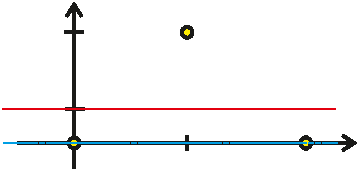
\includegraphics[width = 13cm]{pictures/picture_1_F.pdf}};
    \draw [color = red](4.5,-0.2) node[anchor = north west] {LS line};
    \draw [color = blue](4.5,-1.3) node[anchor = north west] {MAD line};
    \draw [color = black](4.45,-2.5) node[anchor = north west] { $1$ };
    \draw [color = black](-4.5,-2.45) node[anchor = north west] { $0$ };
    \draw [color = black](0,-2.35) node[anchor = north west] { $\frac{1}{2}$ };
    \draw [color = black](-4.55,1.8) node[anchor = north west] { $\frac{1}{2}$ };
    \draw [color = black](-4.55,-1) node[anchor = north west] { $\frac{1}{6}$ };
    \end{tikzpicture}
\end{center}

\begin{remark}
I když $s^2_n$ je nestranný odhad $\sigma^2$, $s_n$ je vychýlený odhad $\sigma$!
Je to obecná vlastnost odhadů (nestranných) rozptylů, neboť pokud je $s^2$ nestranný odhad $\sigma^2$, pak $\E[s] \leq \sigma$.
\end{remark}
\begin{proof}
Uvažujme náhodnou veličinu $X$, pro~kterou platí, že $\D [X] < + \infty$. Po dosazení $X = s$ do známé rovnice $ \E [X^2] = \D [X] +  \E [X]^2$ dostaneme vztah $$\E [s^2] = \D [s] +  \E [s]^2,$$ kde $\E [s]^2 \leq \sigma^2$, $\E [s] \leq \sigma$ a rovnost nastává, pokud $\D [s] = 0$.

\end{proof}
Například pro~normální chyby je $s_n^2 \, \propto \, \chi^2 \Rightarrow \E [s_n] < \sigma$.

\begin{remark}
Předpokládali jsme, že hodnoty $x_i$ jsou dány přesně, což nemusí být vždy pravda. Často jsou obě veličiny $(x,y)$ měřeny nepřesně. Existují EIV models \uv{error in variable}, v~těchto modelech jsou často preferovány jiné odhady než LSE. Populární metoda je dále \textbf{total least squares} (\textit{ortogonal least squares}). Zde minimalizujeme $\sumin d_i^2$, kde $d_i$ je vzdálenost bodu a~přímky (kolmice na~přímku protínající bod). To znamená, že neupřednostňujeme veličinu $x$, ale přistupujeme k~$x$ a~$y$ rovnoměrně.
\end{remark}

\begin{center}
    \begin{tikzpicture}
    \node[inner sep = 0pt] (pic) at (0,0)
    {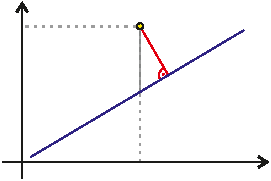
\includegraphics[width = 13cm]{pictures/picture_2_F.pdf}};
    \draw [color = red](1.0,2.3) node[anchor = north west] { $d_i$ };
    \draw [color = red](2.0,1.0) node[anchor = north west] {TLS vzdálenost};
    \draw [color = gray!20!black](-2.6,1.7) node[anchor = north west] {LS vzdálenost};
    \draw [color = red!20!black](0.0,3.80) node[anchor = north west] { $(x_i,y_i)$ };
    \draw [color = black](5.45,-3.65) node[anchor = north west] { $x$ };
    \draw [color = black](0,-3.65) node[anchor = north west] { $x_i$ };
    \draw [color = black](-6.25,3.8) node[anchor = north west] { $y$ };
    \draw [color = black](-6.25,3.3) node[anchor = north west] { $y_i$ };
    \end{tikzpicture}
\end{center}

\begin{remark}
V literatuře se~někdy $x$ uvažují jako realizace náhodné veličiny (ne vždy se~$x$ nastavuje předem, nebo je jasně dané).
\end{remark}
Model má potom tvar
 $$
 \E [Y_i | X_i] = \beta_0 + \beta_1 X_i, \quad  \D [Y_i | X_i] = \sigma^2.
 $$
Pro většinu výsledků prezentovaných v~této přednášce ale není podstatné, zda je $x$ chápáno jako pevné nebo náhodné.
Důkazy většinou fungují s~podmíněnými výrazy $(\E, \D,...)$ při~dané hodnotě $x$ místo~nepodmíněných.
Větší pozornost je naproti tomu potřeba u~odvození asymptotických rozdělení odhadů.

\subsection{Vlastnosti odhadů $\widehat{\beta}_0,~ \widehat{\beta}_1, ~ s_n^2$}
\begin{theorem}
   Nechť $\widehat{\beta}_0, \widehat{\beta}_1$ jsou $\mathrm{LSE}$ odhady parametrů $\beta_0, \beta_1$ v~lineárním modelu
 $$
   		Y_i = \beta_0 + \beta_1 x_i + e_i, \quad i\in\widehat{n},
 $$
   kde $e_i$ jsou nezávislé náhodné veličiny (postačí i~nekorelovanost) se~stejným rozptylem $\sigma^2$. Potom platí, že
   \begin{enumerate}
  \item $\E [\widehat{\beta}_0] = \beta_0, \quad \E [\widehat{\beta}_1] = \beta_1$, (nestranné odhady),
  \item $\D [\widehat{\beta}_1] = \frac{\sigma^2}{\Sxx} , \quad$ kde $ \Sxx = \sumin (x_i - \oxnn)^2$,
  \item $\D [\widehat{\beta}_0] = \sigma^2 \left(\frac{1}{n} + \frac{\oxnn^2}{\Sxx} \right)$.
  \item Pokud navíc platí, že $e_i \sim \NN (0, \sigma^2), ~ \forall i\in\widehat{n}, \quad$ potom $\quad \widehat{\beta}_j \sim \NN (\beta_j, \D [\widehat{\beta}_j]), ~ j \in \{0, 1\}$.
\end{enumerate}
\begin{proof}
   \begin{enumerate}
  \item Upravíme $\widehat{\beta}_1$:
  		\begin{align}
  		    \widehat{\beta}_1 & = \frac{\sumin y_i x_i - n \overline{x}_n \overline{y}_n}{\sumin x_i^2 - n \overline{x}_n^2} = \frac{\sumin (x_i - \oxnn)(y_i - \oynn)}{\sumin (x_i - \oxnn)^2} = \notag \\
  		    & = \frac{1}{\Sxx} \left(\sumin (x_i - \oxnn) y_i - \oynn \sumin (x_i - \oxnn)  \right) = \frac{1}{\Sxx} \sumin (x_i - \oxnn) y_i. \label{Vzorec: beta1}
  		    \end{align}
  		Střední hodnota $\widehat{\beta}_1$ má potom tvar
  		\begin{equation*}
  		\begin{aligned}
  		    \E [\widehat{\beta}_1] & = \E \left[\frac{1}{\Sxx} \sumin (x_i - \oxnn) Y_i \right] = \frac{1}{\Sxx} \sumin (x_i - \oxnn) \E [Y_i]
  		 = \frac{1}{\Sxx} \sumin (x_i - \oxnn) (\beta_0 + \beta_1 x_i) = \\ & = \frac{\beta_0}{\Sxx} \underbrace{\sumin (x_i - \oxnn)}_{ = 0} + \frac{\beta_1}{\Sxx} \sumin (x_i - \oxnn) x_i = \frac{\beta_1}{\Sxx} \underbrace{\sumin (x_i - \oxnn)(x_i - \oxnn)}_{\text{přičítáme 0}} = \frac{\beta_1}{\Sxx} \Sxx = \beta_1
  		    \end{aligned}
  		\end{equation*}
  		a střední hodnota pro~$\widehat{\beta}_0$ má tvar
  		\begin{equation*}
  		\begin{aligned}
  		    \E [\widehat{\beta}_0] = \E [\oyn - \widehat{\beta}_1 \oxn] = \E [\oyn] - \oxnn \E [\widehat{\beta}_1] = \frac{1}{n} \sumin \E [Y_i] - \oxnn \beta_1 = \beta_0 + \frac{\beta_1}{n} \sumin x_i - \oxnn \beta_1 = \beta_0.
  		    \end{aligned}
  		\end{equation*}
  \item 
  Jelikož $Y_i$ jsou nezávislé, můžeme spočítat rozptyl jako
  \begin{equation*}
  			\D [\widehat{\beta}_1] = \D \left[\frac{1}{\Sxx} \sumin (x_i - \oxnn) Y_i \right] = \frac{1}{\Sxx^2} \sumin (x_i - \oxnn)^2 \D [Y_i] = \frac{\sigma^2 \Sxx}{\Sxx^2} = \frac{\sigma^2}{\Sxx}
  		\end{equation*}
  \item  
  Zde už nemáme nezávislé náhodné veličiny, proto musíme počítat i s kovariancí:
  \begin{equation*}
  \begin{aligned}
 \D [\widehat{\beta}_0] & = \D [\oyn - \widehat{\beta}_1 \oxnn] = \D [\oyn] + \oxnn^2 \D [\widehat{\beta}_1] - 2 \oxnn \Cov(\oyn, \widehat{\beta}_1) = \\
  	& = \frac{\sigma^2}{n} + \frac{\oxnn^2 \sigma^2 }{\Sxx} - 2 \oxnn \Cov(\oyn,  \widehat{\beta}_1). 
  	\end{aligned}
  	\end{equation*}
  	Teď už nám stačí ukázat, že $\Cov(\oyn,  \widehat{\beta}_1) = 0$.
  	\begin{equation*}
  	\begin{aligned}
\Cov(\oyn,  \widehat{\beta}_1) & = \Cov \left(\oyn, \frac{1}{\Sxx} \sumin (x_i - \oxnn) Y_i \right) = \frac{1}{\Sxx} \sumin (x_i - \oxnn) \Cov (\oyn, Y_i),  \\
\Cov (\oyn, Y_i) & = \Cov \left(\frac{1}{n} \sumjn Y_j, Y_i\right) = \frac{1}{n} \sumjn \Cov (Y_j, Y_i) = \frac{1}{n} \Cov (Y_i, Y_i) = 	\frac{1}{n} \D Y_i = \frac{\sigma^2}{n}.	
  			\end{aligned}
  		\end{equation*}
  		Z toho už vyplývá, že $$\Cov(\oyn,  \widehat{\beta}_1) = 0 = \frac{\sigma^2}{n \Sxx} \sumin (x_i - \oxnn).$$
  \item Protože
  \begin{align*}
  \widehat{\beta}_1& = \frac{1}{\Sxx}\sumin (x_i-\oxnn)Y_i,\\\widehat{\beta}_0& = \frac{1}{n}\sumin Y_i - \widehat{\beta}_1 \oxnn,
  \end{align*}
  pak je $\widehat{\beta}_0$ i $\widehat{\beta}_1$ LK nezávislých normálních náhodných veličin $Y_i$. Z toho vyplývá, že mají normální rozdělení, kde $\E$ a $\D$ jsme už vypočítali.
\end{enumerate}
\end{proof}
\end{theorem}



\begin{theorem}
	Za předpokladu předchozí věty platí
	 $$
		\E (s_n^2) = \sigma^2,
	 $$
	tedy $s_n^2$ je nestranný odhad $\sigma^2$.
\end{theorem}


\begin{proof}
	 $$
		\E(s_n^2) = \frac{1}{n-2} \E \sumin (Y_i - \hYi)^2 = \frac{1}{n-2} \underbrace{\sumin \E (Y_i - \hYi)^2}_{\text{ozn. } A}.
	 $$
	Protože $\E(\hYi) = \E(\wbeta_0 + \wbeta_1 x_i) = \beta_0 + \beta_i x_i = \E Y_i$, platí, že
	 $$
	\E(Y_i - \hYi)^2 = \D(Y_i - \hYi) = \E (Y_i - \hYi)^2 - \underbrace{\left(\E(Y_i - \hYi)\right)^2}_{ = 0}.
	 $$
	Dostáváme tak	
	\begin{align}
		A & = \sumin \D(Y_i - \hYi) = \sumin [\D(Y_i) + \D(\hYi) - 2 \Cov(Y_i, \hYi)] = \notag \\
		& = n \sigma^2 + \sumin \D(\hYi) - 2 \sumin \Cov(Y_i, \hYi) \label{Vzorec: A}
	\end{align}
	
	Rozepíšeme
	 $$
		\D \hYi = \D(\wbeta_o + \wbeta_1 x_i) = \D \wbeta_0 + x_i^2 \D \wbeta_1 + 2 x_i \Cov (\widehat{\beta}_0,\widehat{\beta}_1),
	 $$
	kde
	 $$
		\Cov(\wbeta_0, \wbeta_1) = \Cov(\lY  - \wbeta_1 \lxn, \wbeta_1) = \underbrace{\Cov(\oy, \wbeta_1)}_{ = 0 \text{ (viz. dříve)}} - \lxn \underbrace{\D(\wbeta_1)}_{\frac{\sigma^2}{\Sxx}} = -\frac{\sigma^2 \lxn}{\Sxx},
	 $$
	a tedy
	\begin{align*}
		\D \hYi & = \sigma^2 \left[\frac{1}{n} + \frac{\lxn^2}{\Sxx} + x_i^2 \frac{1}{\Sxx} - \frac{2 x_i \lxn}{\Sxx} \right] = \sigma^2 \left[\frac{1}{n} + \frac{(x_i - \lxn)^2}{\Sxx}\right], \\
		\sumin \D \hYi & = \sigma^2 + \frac{\sigma^2}{\Sxx} \underbrace{\sumin (x_i - \lxn)^2}_{ = \Sxx} = 2\sigma^2.
	\end{align*}
	
	Následně máme
	\begin{align*}
	\Cov(Y_i, \hYi) & = \Cov(Y_i, \wbeta_0 + \wbeta_1 x_0) = \Cov(Y_i, \wbeta_0) + x_i \Cov(Y_i, \wbeta_1), \\
	\Cov(Y_i, \wbeta_1) & = \frac{1}{\Sxx} \sumjn (x_j - \lxn) \underbrace{\Cov(Y_i, Y_j)}_{ = 0 \text{ pro~} i\neq j} = \frac{\sigma^2(x_i - \lxn)}{\Sxx}, \\
	\Cov(Y_i, \wbeta_0) & = \Cov(Y_i, \overline{Y}_n - \lxn \wbeta_1) = \Cov(Y_i, \overline{Y}) - \lxn \Cov(Y_i, \wbeta_1) = \frac{\sigma^2}{n} - \frac{\lxn \sigma^2 (x_i - \lxn)}{\Sxx}, 
	\end{align*}
	kde za $\wbeta_1$ dosadíme podle \eqref{Vzorec: beta1}. Tedy
	\begin{align*}
		\Cov(Y_i, \hYi) & = \frac{\sigma^2}{n} - \frac{\lxn \sigma^2 (x_i - \lxn)}{\Sxx} + \frac{x_i \sigma^2 (x_i - \lxn)}{\Sxx} = \frac{\sigma^2}{n} + \frac{\sigma^2}{\Sxx}(x_i - \lxn)^2, \\
		\sumin \Cov(Y_i, \hYi) & = \sigma^2 + \frac{\sigma^2}{\Sxx} \sumin (x_i - \lxn)^2 = 2 \sigma^2. 
	\end{align*}
	Dosazením do \eqref{Vzorec: A} dostaneme
	 $$
		A = n\sigma^2 + 2\sigma^2 - 4\sigma^2
	 $$
	a celkem máme
	 $$
		\E(s_n^2) = \frac{1}{n-2} A~ = \sigma^2.
	 $$
\end{proof}

\begin{corollary}\label{tvrzeni}
	Nechť platí předpoklady věty 1 a~nechť $e_1,..., e_n~iid~\NN(0,\sigma^2)$. Potom platí, že
	\begin{enumerate}[a)]
		\item $\frac{(n-2)s_n^2}{\sigma^2} \sim \chi(n-2)$
		\item $s_n^2$ je nezávislé na~$\wbeta_0$ a~$\wbeta_1$.
	\end{enumerate}
\end{corollary}
\begin{proof}
	Vyplyne z~obecnějších tvrzení pro~vícerozměrnou regresi.
\end{proof}


\begin{remark}
	Spočetli jsme
	 \begin{align}
		\widehat{\sigma}^2(\wbeta_0) & \equal{ozn.}\D(\wbeta_0) = \sigma^2 \left[\frac{1}{n} + \frac{\lxn^2}{\Sxx} \right], \label{Vzorec: sigma(beta_0)} \\
		\widehat{\sigma}^2(\wbeta_1) & \equal{ozn.}\D(\wbeta_1) = \frac{\sigma^2}{\Sxx}. \label{Vzorec: sigma(beta_1)}
	 \end{align}
	
	Nestranné odhady jsou
	$$
		\sigma^2(\wbeta_0) = s_n^2  \left[\frac{1}{n} + \frac{\lxn^2}{\Sxx} \right] = s_n^2 \delta_0 \qquad\text{a}\qquad
		\sigma^2(\wbeta_1) = \frac{s_n^2}{\Sxx} = s_n^2 \delta_1,
	$$
	kde $\delta_0$ a~$\delta_1$ jsou tzv. \textit{variance multiplication factors}.
	
	Odhady směrodatné odchylky veličin $\wbeta_0$ a~$\wbeta_1$ pak jsou
	 $$
		\widehat{\sigma}(\wbeta_0) = s_n \sqrt{\delta_0} \qquad \text{a} \qquad \widehat{\sigma}(\wbeta_1) = s_n \sqrt{\delta_1},
	 $$
	kterým se~pak říká standardní chyby odhadů $\wbeta_0$ a~$\wbeta_1$. Hrají zásadní roli při~konstrukci IS a~TH.
\end{remark}

\section{Gauss - Markov theorem}

\begin{itemize}
	\item Pokud mají chyby normální rozdělení, pak LSE pro~$\wbeta_0, \wbeta_1$ je MLE parametrů (eficientní odhad).
	\item Pokud nejsou chyby normální, jaké je opodstatnění použít LSE?
	
	Ukážeme, že LSE jsou BLUE (best linear unbiased estimators), tedy lineární nestranné odhady s~minimálním rozptylem
	\item Je ale třeba poznamenat, že můžou existovat nelineární nebo vychýlené odhady parametrů $\beta_0, \beta_1$, které jsou eficientnější než LSE, pokud se~rozdělení chyb liší výrazně od~normálního (tím se~zabývá robustní regresní analýza).
\end{itemize}

Uvažujme model
 \begin{equation}
	Y_i = \beta_0 + \beta_1 x_i + e_i, \quad i\in\widehat{n}. \tag{$*$} \label{Model 1D LR}
 \end{equation}

\begin{define}
	Lineární odhad parametru $\beta$ je statistika tvaru
	 $$
		\wbeta = \sumin c_i Y_i,
	 $$
	kde $c_i$ jsou dané reálné konstanty a~$i  \in\widehat{n} $.
\end{define}

\begin{theorem}[Gauss-Markov theorem]
	Nechť $e_1,..., e_n$ v~modelu \eqref{Model 1D LR} jsou nekorelované a~mají stejný rozptyl $\D(e_i) = \sigma^2,~ i\in\widehat{n} $. Potom LSE $\wbeta_j,~j\in\{0,1\}$ je BLUE parametru $\beta_j$.
	
\begin{proof}
	Ukážeme pro~$\beta_1$, pro~$\beta_0$ je důkaz podobný. Nechť tedy $\wbeta_1 = \sumin c_i Y_i$, pak	
	 $$\D \wbeta_1 = \sumin c_i^2 \D Y_i = \sigma^2 \sumin c_i^2.$$	
	Aby byl $\wbeta_1$ nestranný, musí platit $\E \wbeta_1 = \beta_1$, tedy
	$$\E \wbeta_1 = \sumin c_i \E Y_i = \beta_0 \sumin c_i + \beta_1 \sumin c_i x_i \overset{!}{ = } \beta_1.$$
	To musí platit pro~libovolná $\beta_0, \beta_1$, a proto dostáváme
	 $$
		\sumin c_i = 0 \quad \text{a} \quad \sumin c_i x_i = 1.
	 $$
	
	Hledání lineárního nestranného odhadu $\beta_1$ je tedy redukováno na~minimalizaci $\sumin c_i^2$ za~vazebných podmínek $\sumin c_i = 0$ a $\sumin c_i x_i = 1$.
	
	Sestavíme Lagrangeovu funkci $L = \sumin c_i^2 - 2 \lambda_1 \left(\sumin c_i\right) - 2 \lambda_2 \left(\sumin c_i x_i - 1\right)$ (konstanta 2 před $\lambda_i$ je zde z toho důvodu, aby výpočet vypadal lépe, ale není nutná).
	
	\begin{align*}
		\frac{\partial L}{\partial c_i} & = 2 c_i - 2 \lambda_1 - 2 \lambda_2 x_i = 0, \quad i\in\widehat{n}, \\
		\frac{\partial L}{\partial \lambda_1} & = -2 \left(\sumin c_i\right) = 0, \\
		\frac{\partial L}{\partial \lambda_2} & = -2 \left(\sumin c_i x_i - 1\right) = 0.
	\end{align*}
	
	Sečteme prvních $n$ rovnic:
	 $$
		\underbrace{\sumin c_i}_{ = 0} - n \lambda_1 - \lambda_2 \sumin x_i = 0 \quad\Rightarrow\quad n\lambda_1 + \lambda_2 \sumin x_i = 0 \quad \Rightarrow \quad\lambda_1 = - \lambda_2 \lxn.
	 $$
	
	Sečteme dále prvních $n$ rovnic vynásobených $x_i$:
	\begin{align*}
		\sumin c_i x_i - \lambda_1 \sumin x_i - \lambda_2 \sumin x_i^2 = 0, \\
		 \lambda_1 \sumin x_i + \lambda_2 \sumin x_i^2 = 1, \\
		 -\lambda_2 \lxn \cdot n \lxn + \lambda_2 \sumin x_i^2 = 1, 
	\end{align*}
	$$\lambda_2 \left(\sumin x_i^2 - n \lxn^2 \right) = 1 \qquad\Rightarrow\qquad \lambda_2 = \frac{1}{\Sxx} \quad \text{a} \quad \lambda_1 = - \frac{\lxn}{\Sxx}.$$
	
	Dosadíme za~$\lambda_1, \lambda_2$ a dostaneme
	 $$
		c_i + \frac{\lxn}{\Sxx} - \frac{x_i}{\Sxx} = 0 \qquad\Rightarrow\qquad c_i = \frac{x_i - \lxn}{\Sxx}\quad\text{a}\quad\wbeta_1 = \frac{1}{\Sxx} \sumin (x_i - \lxn) Y_i,
	 $$
	 což je LSE.

\end{proof}
\end{theorem}

\begin{remark}
	Ukázali jsme pouze, že to je stacionární bod, že je tam i~minimum ukážeme v~obecnější větě ve~vícerozměrné regresi.
\end{remark}

\section{IS pro~$\beta_0, \beta_1$ }
	 IS poskytují jistou \uv{míru přesnosti} bodových odhadů.
	 Pro~jejich konstrukci ale potřebujeme znát rozdělení pravděpodobnosti bodového odhadu.
	 Budeme tedy uvažovat normalitu chyb.
	 Spočtené IS se ale často používají, i~když rozdělení chyb není normální, jejich použití se zdůvodňuje tím, že LSE odhady paramatru $\beta$ jsou lineární funkcí $Y_i, i\in\widehat{n} $, což umožňuje aplikovat CLT a~dostat asymptotickou normalitu odhadů $\wbeta_0, \wbeta_1$.

Uvažujme model $Y_i = \beta_0 + \beta_1 x_i + e_i$, $e_i~iid~\NN(0,\sigma^2)$. Víme, že
 $$
	\wbeta_i \sim \NN\left(\beta_i, \sigma^2(\wbeta_i)\right), \quad \frac{(n-2)s_n^2}{\sigma^2} \sim \chi^2(n-2) \text{ a~nezávisí na~} \wbeta_0, \wbeta_1.
 $$

\begin{remark}
	 $$
		X \sim \NN(0,1),\quad Y \sim \chi^2(n), \quad X, Y \text{ nezávislé } \Rightarrow \frac{X}{\sqrt{Y/n}} \sim t(n)
	 $$
\end{remark}

Můžeme ukázat, že 
 $$
	T_i : = \frac{\frac{\wbeta_i - \beta_i}{\sigma(\wbeta_i)}}{\frac{s_n}{\sigma}} = \frac{\wbeta_i - \beta_i}{\widehat{\sigma}(\wbeta_i)} \sim t(n-2),\quad i\in\{0,1\},
 $$
neboť $\sigma(\wbeta_i) = \sigma \sqrt{\delta_i}$ a~$\widehat{\sigma}(\wbeta_i) = s_n \sqrt{\delta_i}$.

To znamená, že $\PP\left[-t_{1-\frac{\alpha}{2}}(n-2) \leq \frac{\wbeta_i - \beta_i}{\widehat{\sigma}(\wbeta_i)} \leq t_{1-\frac{\alpha}{2}}(n-2) \right] = 1-\alpha$. Vyjádřením $\beta_i$ dostaneme
 $$
	\PP\left[\wbeta_i - t_{1-\frac{\alpha}{2}}(n-2) \widehat{\sigma}(\wbeta_i) \leq \beta_i \leq  \wbeta_i + t_{1-\frac{\alpha}{2}}(n-2) \widehat{\sigma}(\wbeta_i) \right] = 1 - \alpha,
 $$
a tedy $\left(\wbeta_i \pm t_{1-\frac{\alpha}{2}}(n-2) \widehat{\sigma}(\wbeta_i)\right)$ je $100(1-\alpha)\%$ IS pro~$\beta_i,~ i\in\{0,1\}$.

Dosazením za~$\widehat{\sigma}(\wbeta_i)$ dostaneme

\begin{itemize}
	\item $100(1-\alpha)\%$ IS pro~$\beta_0$ : $\wbeta_0 \pm t_{1-\frac{\alpha}{2}}(n-2) \cdot s_n \sqrt{\frac{1}{n} + \frac{\lxn^2}{\Sxx}}$
	\item $100(1-\alpha)\%$ IS pro~$\beta_1$ : $\wbeta_1 \pm t_{1-\frac{\alpha}{2}}(n-2) \cdot s_n \frac{1}{\sqrt{\Sxx}}$
\end{itemize}

\begin{remark}
	Z tvarů IS lze pozorovat, že IS pro~$\beta_0$ bude ve~většině praktických případů širší, než IS pro~$\beta_1$, tzn. směrnice je obecně odhadnuta s~větší přesností, než absolutní člen (intercept).
\end{remark}


\begin{remark}
	Někdy se~konstruují simultánní IS pro~oba parametry.

\begin{center}

    \begin{tikzpicture}
    \node[inner sep = 0pt] (pic) at (0,0)
    {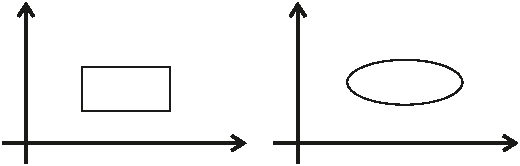
\includegraphics[width = 13cm]{pictures/picture_5_M.pdf}};
    \draw [color = black](-6.75,2.4) node[anchor = north west] { $\beta_0$ };
    \draw [color = black](0,2.4) node[anchor = north west] { $\beta_0$ };
    \draw [color = black](-1.2,-1.6) node[anchor = north west] { $\beta_1$ };
    \draw [color = black](5.45,-1.6) node[anchor = north west] { $\beta_1$ };
    \draw [color = black](2.9,0.25) node[anchor = north west] { $1 - \alpha$ };
    \draw [color = black](-3.9,0.2) node[anchor = north west] { $1 - \alpha$ };
    \end{tikzpicture}
\end{center}	
	
	 Zmíníme podrobněji u~vícerozměrné regrese.
\end{remark}


\section{Testování hypotéz pro~$\beta_0, \beta_1$ }

Chtěli bychom ověřit platnost předpokladu lineárního vztahu mezi~$x$ a~$y$.

Předpokládejme nyní, že model je lineární, a že $x$ je jediná dostupná vysvětlující proměnná. Otázkou zůstává, zda je $x$ užitečná ve~vysvětlení variability v~$y$, chceme tedy rozhodnout mezi~dvěma modely:
 $$
	Y_i = \beta_0 + e_i \quad \text{a} \quad Y_i = \beta_0 + \beta_1 x_i + e_i,
 $$
tzn. otestovat hypotézu $\hypothesis{\beta_1 = 0}{}\beta_1 \neq 0$.

Pokud nezamítneme $H_0$, závěr bude, že $x$ nevysvětluje nic z~variability $y$ a~není v~modelu významné. Pokud zamítneme $H_0$, znamená to, že $x$ je významné.

\begin{remark}
	Tyto závěry jsou správné pouze za~předpokladu, že model je lineární!
	\begin{itemize}
		\item Nezamítnutí $H_0$ nemusí znamenat, že $x$ není užitečná, může to pouze indikovat, že vztah mezi~$y$ a~$x$ není lineární.
		\item Zamítnutí $H_0$ naopak říká, že existuje lineární trend mezi~$x$ a~$y$, ale mohou tam být i~jiné typy závislostí.
	\end{itemize}
\end{remark}

Pro konstrukci testů využijeme odvozené IS.

\begin{remark}
	Opakování: $\hypothesis{\theta = \theta_0}{\theta \neq \theta_0} \Rightarrow (\underline{\theta}, \overline{\theta})$ je $100(1-\alpha)\%$ IS pro~$\theta$. Pak $W = \{ x | \theta_0 \notin (\underline{\theta}, \overline{\theta}) \}$ je kritický obor testu na~hladině $\alpha$.
\end{remark}

 $H_0: \beta_1 = 0$ zamítneme, pokud $0 \notin \left(\wbeta_1 \pm t_{1-\frac{\alpha}{2}}(n-2) \cdot  \frac{s_n}{\sqrt{\Sxx}} \right)$, tzn.
\begin{align*}
	\text{buď } \wbeta_1 + t_{1-\frac{\alpha}{2}}(n-2) \cdot  \frac{s_n}{\sqrt{\Sxx}} < 0 \quad\Leftrightarrow\quad \wbeta_1 \frac{\sqrt{\Sxx}}{s_n} < - t_{1-\frac{\alpha}{2}}(n-2) \\
	\text{nebo } \wbeta_1 - t_{1-\frac{\alpha}{2}}(n-2) \cdot  \frac{s_n}{\sqrt{\Sxx}} > 0 \quad\Leftrightarrow\quad \wbeta_1 \frac{\sqrt{\Sxx}}{s_n} > t_{1-\frac{\alpha}{2}}(n-2).
\end{align*}
A zapsáno dohromady
 $$
	|T_n| = |\wbeta_1| \frac{\sqrt{\Sxx}}{s_n} > t_{1-\frac{\alpha}{2}}(n-2).
 $$

\begin{remark}
	Intuitivní interpretace: $|T_n| = |\wbeta_1| \frac{\sqrt{\Sxx}}{s_n} = \frac{|\wbeta_1|}{\widehat{\sigma}(\wbeta_1)}$ je převrácená hodnota relativní chyby.
	
	Pokud je $\beta_1$ dobře odhadnuto, očekáváme malý rozptyl $\widehat{\sigma}(\wbeta_1)$, tedy $T$ bude velké.
	
	t-test tedy říká, že zamítneme $H_0$, pokud je relativní chyba odhadu malá.
\end{remark}% pages 21-30
\begin{remark}
	Někdy dopředu známe kandidáta $b_1$ jako hodnotu parametru $\beta_1$ a~chtěli bychom testovat
	 $\hypothesis{\beta_1 = b_1}{\beta_1\neq b_1}$. Test tedy zamítá $H_0$, pokud
	 $$ \abs{\beta_1-b_1}\cdot \frac{\sqrt{\Sxx}}{s_n}> t_{1-\frac{\alpha}{2}}(n-2). $$
\end{remark}
\subsubsection*{Test významnosti interceptu}
Otázka je, zda přímka prochází počátkem $(0,0)$, tedy $\hypothesis{\beta_0 = 0}{\beta_0\neq0}$. Nezamítnutí $H_0$ znamená, že jednodušší model $y = \beta_1 x+e$ lépe popisuje data, než $y = \beta_0+\beta_1 x+e$. $H_0$ potom zamítneme, pokud
 $$ T_n = \frac{|\widehat{\beta}_0|}{\widehat{\sigma}(\widehat{\beta}_0)} = |\widehat{\beta}_0|\frac{1}{s_n\sqrt{\frac{1}{n}+\frac{\overline{x}^2}{\Sxx}}}>t_{1-\frac{\alpha}{2}}(n-2). $$

\section{ANOVA přístup pro~testování}
Odvodili jsme t-test významnosti koeficientů a~nyní odvodíme ekvivalentní F-test, který může být zobecněn na~test celkové významnosti vícerozměrného regresního modelu (testy významnosti jednotlivých koeficientů mohou být totiž zavádějící).

Myšlenkou metody (analýza rozptylu ANOVA) je určit, kolik variability v~pozorováních $(y_1,y_2,...,y_n)$ je \uv{vysvětleno} regresním modelem (přímkou). Míru variability v~datech pak spočítáme jako podíl součtu sum od~regrese a~celkového počtu čtverců, tedy
 $$ \SST = \sumin(y_i-\overline{y}_n)^2, $$
pokud regresní přímka $y = \widehat{\beta}_0+\widehat{\beta}_1 x$ dobře prokládá data, tedy $\widehat{y}_i\approx y_i$. Dále bude platit, že
 $$ \sumin (\hyi-\lhyn)^2\approx\sumin (y_i-\lyn)^2. $$
Ukážeme, že $\lhy_n = \lyn$, a~tak
 $$ \sumin (\hyi-\lhyn)^2 = \sumin (\hyi-\lyn)^2 = \SSR, $$ což značí \textit{regression sum of squares} (regresní součet čtverců). Podíl
 $$ \RMR^2 = \frac{\SSR}{\SST} = \frac{\sumin (\hyi-\lyn)^2}{\sumin (y_i-\lyn)^2} $$ tak vyjadřuje podíl variability v~$(y_1,...,y_n)$ vysvětlené regresním modelem. Statistika $\RMR^2$ se nazývá \textbf{koeficient determinace} \textit{(coefficient of determination)} a pro každý model by měla mít hodnotu $\RMR^2\approx 1$.

Ukážeme, že $\RMR^2$ je kvadrát výběrového korelačního koeficientu mezi~$\textbf{x}$ a~$\textbf{y}$, což dává statistice $\RMR^2$ význam míry \uv{dobré shody}.

Pokud bychom znali rozdělení pravděpodobnostní statistiky $\RMR^2$, nabízí se~její použití pro~test $H_0:~\beta_1 = 0$, kterou bychom zamítli, pokud bude $\RMR^2\approx1$. Protože každá monotonní funkce $\RMR^2$ vede na~ekvivalentní test, budeme uvažovat statistiku 
\begin{equation}
	F = \frac{(n-2)\RMR^2}{1-\RMR^2}. \label{Definice F}
	\end{equation}

\begin{lemma}\label{lemma_k_vete}
	Nechť $\widehat{e}_i = y_i-\hyi$ značí rezidua, kde $\hyi = \wbeta_0+\wbeta_1 x_i$ a~$\wbeta_0,\wbeta_1$ jsou LSE. Potom \begin{enumerate}
		\item $\sumin \widehat{e}_i = 0$,
		\item $\lhyn = \lyn$,
		\item $\sumin \widehat{e}_i\hyi = 0$.
	\end{enumerate}
\begin{proof}
	\begin{enumerate}
		\item Z~rovnice $\frac{\partial S}{\partial\wbeta_0} = 0$ dostaneme $$ 0 = \sumin (y_i-\wbeta_0-\wbeta_1 x_i) = \sumin (y_i-\hyi) = \sumin \widehat{e}_i. $$
		\item Z~bodu 1) plyne, že $\sumin \hyi = \sumin y_i$, podělením $n$ dostaneme dokazované tvrzení.
		\item Z~rovnice $\frac{\partial S}{\partial\wbeta_1} = 0$ dostaneme $$ 0 = \sumin (y_i-\wbeta_0-\wbeta_1 x_i)x_i = \sumin \hei x_i, $$ a~tedy $$ \sumin \hei\hyi = \sumin \hei (\wbeta_0+\wbeta_1 x_i) = \sumin \hei\wbeta_0+\sumin x_i \hei\wbeta_1 = \wbeta_0\underbrace{\sumin \hei}_{ = 0}+\wbeta_1\underbrace{\sumin x_i\hei}_{ = 0} = 0. $$
	\end{enumerate}
\end{proof}
\end{lemma}
\begin{theorem}\label{vetasbysxx}
	Předpokládejme, že $\SST\neq 0$. Potom platí\begin{enumerate}
		\item $0\leq \RMR^2\leq1$,
		\item $\RMR^2 = 1-\frac{\SSE}{\SST}$, kde $\SSE = \sumin (y_i-\hyi)^2$ jako reziduální součet čtverců,
		\item $\RMR^2 = 1~\Leftrightarrow~(\forall i\in\widehat{n})(\hyi = y_i)$ (všechna data leží na~přímce),
		\item pokud označíme $\textbf{x} = (x_1,...,x_n)$ a~$\textbf{y} = (y_1,...,y_n)$, potom $\RMR^2 = \rho^2(\textbf{x},\textbf{y})$, kde $$ \rho(\textbf{x},\textbf{y}) = \frac{ \Big( \sumin (x_i-\overline{x}_n)(y_i-\lyn) \Big)^2}{\Sxx S_{yy}}, $$ tedy $\RMR^2$ je druhá mocnina výběrového korelačního koeficientu vektorů $\textbf{x},\textbf{y}$,
		\item $F = \frac{\SSR}{s_n^2} = \mathrm{T}^2$,
		\item pokud jsou chyby $e_1,...,e_n~iid~\NN(0,\sigma^2)$ a~$\beta_1 = 0$ (platí $H_0:~\beta_1 = 0$) v~modelu, potom $F\sim\FF(1,n-2)$.
	\end{enumerate}
\begin{proof}
	Důkaz věty bude založen na~rozkladu
	 $$ \sumin (y_i-\lyn)^2  = \sumin (\hyi-\ly)^2 + \sumin (y_i-\hyi)^2 \iff \SST = \SSR+\SSE.$$
	 Z~lemmatu \ref{lemma_k_vete} vyplývá, že
	\[
	\begin{split}
	\SST& = \sumin (y_i-\lyn)^2 = \sumin \left[(y_i-\hyi)+(\hyi-\lyn) \right]^2 = \\& = \sumin (y_i-\hyi)^2+\sumin (\hyi-\lyn)^2+2\sumin (y_i-\hyi)(\hyi-\lyn) = \SSE+\SSR+0,
	\end{split}
	\]
	neboť $$ \sumin \underbrace{(y_i-\hyi)}_{ = \hei}(\hyi-\lyn) = \underbrace{\sumin \hei\hyi}_{ = 0}-\lyn\underbrace{\sumin \hei}_{ = 0} = 0. $$
	Z toho potom dokazujeme jednotlivé body věty. \begin{enumerate}
		\item Protože $\SST = \SSE+\SSR$, pak $0\leq \RMR^2 = \frac{\SSR}{\SST}\leq \frac{\SST}{\SST} = 1$.
		\item $\SSR = \SST-\SSE~\Rightarrow~\RMR^2 = \frac{\SST-\SSE}{\SST} = 1-\frac{\SSE}{\SST}$.
		\item Z~bodu 2 plyne, že $\RMR^2 = 1~\Leftrightarrow~\SSE = 0$ a~$\SSE = \sumin (y_i-\hyi)^2 = 0~\Leftrightarrow~y_i = \hyi, ~\forall i\in\widehat{n}$.
		\item Platí $\hyi = \wbeta_0 + \wbeta_1 x_i = \lyn-\wbeta_1 \overline{x}_n + \wbeta_1 x_i = \lyn-\wbeta_1(\overline{x}_n-x_i)$. Proto pak
		$$ \SSR = \sumin (\hyi-\lyn)^2=\wbeta_1^2\sumin (x_i-\overline{x}_n)^2 = \wbeta_1^2 \Sxx, $$
		a~protože $\wbeta_1 = \frac{1}{\Sxx}\sumin (x_i-\overline{x}_n)(y_i-\lyn)$, dostaneme
		 $$ \rho^2(\textbf{x},\textbf{y}) = \frac{\Big[\sumin (x_i-\overline{x}_n)(y_i-\lyn)\Big]^2}{\Sxx S_{yy}} = \frac{\wbeta_1^2 \Sxx}{S_{yy}} = \frac{\SSR}{\SST} = \RMR^2, $$
		 neboť $S_{yy} = \sumin (y_i-\lyn)^2 = \SST$.
		\item Z~definice $F$ podle \eqref{Definice F} plyne, že
		 $$ F = \frac{(n-2)\RMR^2}{1-\RMR^2} = \frac{(n-2)\frac{\SSR}{\SST}}{\frac{\SSE}{\SST}} = \frac{\SSR}{\frac{\SSE}{n-2}} = \frac{\SSR}{s_n^2}. $$ Protože $\mathrm{T}_n = \wbeta_1\frac{\sqrt{\Sxx}}{s_n}$, pak $$ \mathrm{T}^2 = \frac{\wbeta_1^2 \Sxx}{s_n^2} = \frac{\SSR}{s_n^2} = F. $$
		\item $\mathrm{T}\sim t(n-2) \Rightarrow F = \mathrm{T}^2\sim\FF(1,n-2)$.
		
	\end{enumerate}
\end{proof}
\end{theorem}
\begin{remark}
\begin{enumerate}
	\item 	Z bodů 5 a~6 vyplývá, že použití libovolné statistiky $\mathrm{T}_n,\RMR^2$ nebo $F$ vede na~ekvivalentní test významnosti regrese.
	\item $\RMR^2$ poskytuje hrubou představu o~kvalitě modelu, čím je blíže $1$, tím lépe přímka prokládá data (nicméně je třeba jisté obezřetnosti, jak uvidíme později).
	\item $F$ lze chápat jako statistiku pro~test významnosti velkých hodnot $\RMR^2$.
\end{enumerate}
\end{remark}
Výsledky se~většinou uvádí v~tabulce ANOVA:
\begin{table}[h]\label{ANOVA_table}
	\begin{tabular}{|lllll|}
	\hline
	Source & df & SS & MS & $F$\\
	\hline
	Regression & 1 & $\SSR$ & MSR = $\SSR$ & $\frac{\mathrm{MSR}}{\mathrm{MSE}}$ \\
	Residual & $n-2$ & $\SSE$ & $\mathrm{MSE} = \frac{\mathrm{\SSE}}{n-2} = s_n^2$ & \\
	Total & $n-1$ & $\SST$ & & \\ \hline
\end{tabular}
\end{table}

Kde \textbf{Source} je zdroj součtu čtverců, \textbf{df} počet stupňů volnosti příslušný danému součtu čtverců, \textbf{SS} počet čtverců a~\textbf{MS} $(\mathrm{MS} = \frac{\mathrm{SS}}{\mathrm{df}})$ \uv{mean squares}.
\begin{remark}
	 $H_0:\beta_1 = 0$ je zamítnuta, pokud $F>\FF_{1-\alpha}(1,n-2)$. V~tomto jednorozměrném případě je to ekvivalentní t-testu, neboť $F = \mathrm{T}^2$.
\end{remark}
\begin{theorem}
	Mějme $e_1,...,e_n~iid~\NN(0,\sigma^2)$. Za~platnosti $H_0:~\beta_1 = 0$ je splněno, že
	 $$ \frac{\SSR}{\sigma^2}\sim\chi^2(1),\qquad\frac{\SSE}{\sigma^2}\sim\chi^2(n-2),\qquad\frac{\SST}{\sigma^2}\sim\chi^2(n-1). $$
\end{theorem}
\begin{remark}
	Proto se v~tabulce ANOVA \ref{ANOVA_table} uvádí df po~řadě $1,n-2,n-1$. Používají se~však i~v~případě jiného rozdělení chyb. Představit si je lze takto:
	\begin{enumerate}
		\item $\SSE = \sumin \hei^2$, na~$n$ reziduí $\he_1,...,\he_n$ máme 2 podmínky, $\sumin \hei = 0$ a~$\sumin x_i\hei = 0$. Z~toho vyplývá, že mají $n-2$ stupňů volnosti.
		\item $\SST = \sumin (y_i-\lyn)^2$, a proto musí $y_i-\lyn$ splňovat $\sumin (y_i-\lyn) = 0$, tudíž má $n-1$ stupňů volnosti.
		\item $\SSR = \SST-\SSE$ a~počet stupňů volnosti je roven $(n-1)-(n-2) = 1$.
	\end{enumerate}
\begin{proof}
	V důkazu věty \ref{vetasbysxx} jsme ukázali, že $\SSR = \wbeta_1^2 \Sxx$, takže $\frac{\SSR}{\sigma^2} = \left(\frac{\wbeta_1\sqrt{\Sxx}}{\sigma} \right)^2$. Víme, že $\wbeta_1\sim\NN\left(\beta_1,\frac{\sigma^2}{\Sxx}\right)$, a~tedy $(\wbeta_1-\beta_1)\frac{\Sxx}{\sigma}\sim\NN(0,1)$. Pro~$\beta_1 = 0$ tedy $$ \wbeta_1\frac{\sqrt{\Sxx}}{\sigma}\sim\NN(0,1)~\Rightarrow~\frac{\SSR}{\sigma^2}\sim\chi^2(1). $$
	Zároveň také $\frac{\SSE}{\sigma^2} = \frac{(n-2)s_n^2}{\sigma^2}\sim\chi^2(n-2)$ (viz tvrzení \ref{tvrzeni}) a~nezávisí na~$\wbeta_1$. Z~toho vyplývá, že $\frac{\SSR}{\sigma^2}$ a~$\frac{\SSE}{\sigma^2}$ jsou nezávislé. Dále platí, že
	 $$ \frac{\SST}{\sigma^2} = \frac{\SSR}{\sigma^2}+\frac{\SSE}{\sigma^2}~\Rightarrow~\frac{\SST}{\sigma^2}\sim\chi^2(n-1). $$
\end{proof}
\end{remark}
\begin{remark}
	 $\RMR^2$ statistika - pozor na~zjednodušení kvality modelu. \begin{enumerate}
		\item Nízké hodnoty $\RMR^2$ nemusí znamenat, že regresní model není významný. V~datech jen může být velké množství nevysvětlitelné náhodné variability. Například opakování hodnoty regresoru $x$ snižují hodnotu $\RMR^2$ oproti~modelům s~různými $x$.
		\item Velké hodnoty $\RMR^2$ mohou být způsobeny velkým měřítkem dat ($\Sxx$ je velká). Platí totiž, že
		 $$ \E(\RMR^2)\approx\frac{\beta_1^2 \Sxx}{\beta_1^2 \Sxx+\sigma^2}, $$ což je rostoucí funkce $\Sxx$.
		
		Velký rozptyl $(x_1,...,x_n)$ může mít za~následek velké $\RMR^2$ a~přitom nic neříká o~kvalitě modelu.
		
		 $\E(\RMR^2)$ je také rostoucí funkcí $\beta_1^2$. Modely s~velkou směrnicí tedy budou mít obecně větší $\RMR^2$, než modely s~\uv{malou} směrnicí.
	\end{enumerate}
\end{remark}

Při hodnocení kvality modelu potřebujeme více kritérií. Mezi~ně patří například\begin{enumerate}
	\item \uv{velké} $\RMR^2$,
	\item \uv{velké} $F$ nebo $|\mathrm{T}|$ hodnoty,
	\item \uv{malé} hodnoty $s_n^2$ vzhledem k~$\lyn$.
\end{enumerate}
Další kritéria budeme probírat později.
\begin{example}
	Velká hodnota $\RMR^2$ indikuje přibližně lineární vztah mezi~$x$ a~$y$, ale vysoký stupeň korelace nemusí znamenat příčinný vztah.
	Uveďme nyní říklad na datech z let 1924-1937. Mějme
	
	 $y_i$ - počet mentálních onemocnění na~$100000$ obyvatel Anglie.\\
	 $x_i$ - počet rádií v~populaci.\\
	Určíme parametry modelu $y_i = \beta_0+\beta_1 x_i+e_i$ jako
	 $$ \wbeta_0 = 4.5822,\qquad\wbeta_1 = 2.2042,\qquad\RMR^2 = 0.984, $$
	tzv. zjišťujeme velmi významný lineární vztah mezi~$x$ a~$y$. Závěr by mohl být, že rádia způsobují mentální onemocnění. I~když by to mohla být pravda, nabízí se~věrohodnější vysvětlení, a~to takové, že $x$ i~$y$ rostou lineárně s~časem, tzn. $y$ roste lineárně s~$x$.
	
	Rádia byla s~časem dostupnější, lepší diagnostické procedury umožňovaly identifikovat více lidí s~mentálními problémy.
\end{example}
\begin{remark}
Korelace VS příčinnost

 \begin{itemize}
  \item \textbf{Příčinná spojitost} -- i~když je příčinná spojitost mezi~$x$ a~$y$, korelace samotná nám neřekne, zda $x$ ovlivňuje $y$ nebo naopak.
  \item \textbf{Skrytá příčinnost} -- skrytá veličina $z$ ovlivňuje $x$ i~$y$, což způsobuje jejich korelovanost.
  \item \textbf{Confounding factor} -- skryté proměnné $z$ i~$x$ ovlivňují $y$, výsledek tedy závisí i~na~$z$.
  \item \textbf{Coincidence} -- korelace je náhodná.
\end{itemize}
\end{remark}

\section{Regrese skrz~počátek}
Existují případy, kdy přípustný model vyžaduje $\beta_0 = 0$, tj. $
 Y_i = \beta_1 x_i + e_i,~ i\in\widehat{n}$.


 \begin{enumerate}[1.]
  \item Na~základě fyzikálních úvah je předem známo, že
 $$
 \E [Y_0] = \beta_0 = 0.
 $$
		Potom tedy nemá smysl odhadovat $\beta_0$, protože to obecně sníží přesnost odhadu $\sigma^2$, a~tedy i~$\beta_1$.
  \item Na~začátek předpokládáme, že $\beta_0 \neq 0$ a~t-test nezamítne hypotézu $\text{H}_0 : \beta_0 = 0$, potom může být $\beta_0$ z~modelu odstraněn.
\end{enumerate}

\begin{remark}
V praktických situacích si často nemůžeme být jisti, že model platí i~blízko počátku. Část statistiků trvá na~přítomnosti interceptu v~modelu, i~když je nevýznamný.

Položit $\beta_0$ apriorně může být chybné, i~když $\E [Y_0] = 0$. Pokud totiž nevíme jistě, že model je lineární na~okolí 0, volba $\beta_0 = 0$ může vést k~vychýleným odhadům $\beta_1$, pokud jsou nezávislé proměnné daleko od~$x = 0$.
\end{remark}

\subsection{Odhady a~testy v~případě $\beta_0 = 0$ }
LSE parametr $\beta_1$ dostaneme minimalizací $S~ = \sumin (y_i - \beta_1 x_i)^2$ ve~tvaru
 $$
 \widehat{\beta}_1 = \frac{\sumin y_i  x_i }{\sumin x_i^2}.
 $$
Pokud $e_1,..., e_n~iid~\NN(0,\sigma^2)$, potom 
$$\E [\widehat{\beta}_1] = \beta_1\quad\text{a}\quad\D [\widehat{\beta}_1] = \frac{\sigma^2}{\sum_{i=1}^n x_i^2}\quad\Rightarrow\quad\widehat{\beta}_1 \sim \NN\left(\beta_1, \frac{\sigma^2}{\sum_{i=1}^n x_i^2}\right)$$
a $s_n^2 = \frac{1}{n-1}\sumin (y_i -  \widehat{y}_i)^2 = \frac{\SSE}{n-1}$ je nestranný odhad $\sigma^2$.
Dále $\frac{\SSE}{\sigma^2} \sim \chi^2(n-1)$ a~nezávisí na~$\widehat{\beta}_1$.
 $\text{H}_0 : \beta_1 = 0$ lze otestovat za~pomoci statistiky
 $$
  \mathrm{T} = \frac{\widehat{\beta}_1}{\frac{s_n}{\sqrt{\sum x_i^2}}} \sim \mathrm{t}(n-1),
 $$
kde $100(1-\alpha) \%$ IS pro~$\beta_1$ je $$\bigg(\widehat{\beta}_1 \pm \mathrm{t}_{1 - \frac{\alpha}{2}}(n-1)\frac{s_n}{\sqrt{\sum x_i^2}}\bigg).$$

Zatím je vše podobné jako pro~případ $\beta_1 \neq 0$. Rozdíl je ale v~tabulce ANOVA a~v~míře dobré shody. Problém je, že neplatí rozklad $\SST = \SSR + \SSE$, neboť součet reziduí $\sumin (y_i - \widehat{y})$ nemusí být 0, a~tedy $\overline{\widehat{y}}_n \neq \overline{y}_n$. Odvodíme nový rozklad, který platí v~obou případech, dokážeme ho ale jen pro~$\beta_0 = 0$.

\begin{theorem}
V modelu s~$\beta_0 = 0$ platí, že
 $$
 \sumin y_i^2 = \sumin \widehat{y}_i^2 + \sumin (y_i - \widehat{y}_i)^2.
 $$
\end{theorem}

\begin{proof}
 $$
 \sumin y_i^2 = \sumin (y_i - \widehat{y}_i + \widehat{y}_i)^2 = \sumin (y_i - \widehat{y}_i)^2 + \sumin \widehat{y}_i^2 + 2 \sumin (y_i - \widehat{y}_i) \widehat{y}_i
 $$
 Z rovnice $\frac{\d S}{\d \beta_1} = 0$ dostaneme $\sumin (y_i - \widehat{\beta}_1 x_i) x_i = 0
 $ a po vynásobení obou stran rovnic $\wbeta_1$ již máme
 $$
 \sumin (y_i - \widehat{y}_i) \widehat{y}_i = 0.
 $$
\end{proof}
Pokud vezmeme $\sum y_i^2$ jako míru variability v~datech, analogie $\RMR^2$ statistiky bude

 $$
  \RMR^2 = \frac{\sumin \widehat{y}_i^2}{\sumin y_i^2} \quad \Leftrightarrow \quad
  1 - \RMR^2 = \frac{\sumin y_i^2 - \sumin \widehat{y}_i^2}{\sumin y_i^2} = \frac{\sumin \widehat{e}_i^2}{\sumin y_i^2 }
 $$
Definujeme $F : = \frac{(n-1) \RMR^2}{1 - \RMR^2}$. Potom
 $$
  F = \frac{\sumin \widehat{y}_i^2 }{\frac{1}{n-1} \sumin (y_i - \widehat{y}_i)^2 } = \frac{\widehat{\beta}_1 \sumin x_i^2 }{ s_n^2} = \text{T}^2.
 $$
Vztah mezi~$\RMR^2, F$ a $\mathrm{T}^2$ je tedy stejný jako pro~$\beta_0 \neq 0$.

\begin{remark}
  Tato definice $\RMR^2$ se~ale v~praxi moc nepoužívá, protože neumožňuje přímé srovnání modelů s~interceptem a bez něj.
\end{remark}
 $$
  \beta_0 = 0  : \quad \RMR^2 = 1 - \frac{\SSE}{\sumin y_i^2},
\qquad
  \beta_0 \neq 0  : \quad \RMR^2 = 1 - \frac{\SSE}{\sumin (y_i - \oynn)^2}.
 $$

Obecně ale $\sumin (y_i - \oynn)^2 < \sumin y_i^2$, $\RMR^2$ v~modelu s~$\beta_0 = 0$ tedy bude větší, než $\RMR^2$ modelu s~$\beta_0 \neq 0$, i~když jsou jejich $\SSE$ srovnatelné.

\begin{enumerate}[1.]
  \item Definice vhodné $\RMR^2$ pro~$\beta_0 = 0$ vyvolává jistou kontroverzi a~existuje několik verzí.
  \item Možná volba je $\RMR^2 = \left(\rho (y_I, \overline{y}_I)\right)^2$, kde $\overline{y}_I = (\overline{y}_1,...,\overline{y}_n)$, protože tato vlastnost platí i~pro~případ $\beta_0 = 0$.
  \item Další možnost je srovnat modely pomocí hodnot $s_n^2$ (preferujeme~model s~nejnižší hodnotou $s_n^2$).
\end{enumerate}\begin{table}[h]
	\begin{tabular}{lllll}
		Source & df & SS & MS & F \\
		\hline
		Regression & $1$ & $\SSR = \sumin \hyi^2$ & MSR $ = \frac{\SSR}{1}$ & $\frac{\SSR}{s_n^2}$ \\
		Residual & $n-1$ & $\SSE = \sumin (y_i - \hyi)^2$ & MSE $ = \frac{\SSE}{n-1}$ &  \\
		Total & $n$ & $\SST = \sumin y_i^2$ &  &  \\
		\hline
		&  & $\RMR^2 = \rho^2(\textbf{y},\widehat{\textbf{y}})$ &  &  \\
	\end{tabular}
\caption{Tabulka ANOVA pro~$\beta_0 = 0$.}
\end{table}

\section{Predikce}
Jakmile máme model, často bývá cílem odhadnout hodnoty veličiny $Y_0$ pro~nové $x_0$, které není v~původních datech. Budeme uvažovat dva typy predikce:\begin{enumerate}[1)]
	\item predikce střední hodnoty $\mu_0 = \EE{Y_0}$ v~bodě $x_0$,
	\item predikce hodnoty nového pozorování $Y_0$ v~bodě $x_0$.
\end{enumerate}
Pro oba typy použijeme bodový odhad
 $ \widehat{Y}_0 = \wbeta_0+\wbeta_1 x_0. $
Intervalové odhady se~ale budou lišit.

\subsection*{Ad 1)}
	Protože je $\mu_0 = \beta_0+\beta_1 x_0$ vlastně parametr, lze pro~něj odvodit IS (za předpokladu normality chyb).
	Spočteme tedy $\D(\widehat{Y}_0)$. Dosazením odhadů $\wbeta_0$ a~$\wbeta_1$ dostaneme $\widehat{Y}_0 = \overline{y}+\wbeta_1(x_0-\overline{x})$ a
	 $$ \D\widehat{Y}_0 = \D(\overline{Y})+(x_0-\overline{x})^2\D(\wbeta_1)+2(x_0-\overline{x})\underbrace{\Cov(\overline{Y},\wbeta_1)}_{ = 0} = \frac{\sigma^2}{n}+\frac{\sigma^2(x_0-\overline{x})^2}{\Sxx} = \sigma^2\left[\frac{1}{n}+\frac{(x_0-\overline{x})^2}{\Sxx} \right]. $$
	
	Nahrazením $\sigma^2$ statistikou $s_n^2$ dostaneme odhad $\D(\widehat{Y}_0)$ ve~tvaru
	 $$ \widehat{\sigma}^2(\widehat{Y}_0) = s_n^2\left[\frac{1}{n}+\frac{(x_0-\lx)^2}{\Sxx} \right]. $$
	 $\wsigma(\hY_0)$ se~obvykle nazývá \textbf{standardní chyba predikce v~bodě $x_0$ }. Jsou-li $e_1,...,e_m~iid~\NN(0,\sigma^2)$, platí, že
	 $$ \hY_0\sim\NN\bigg(\mu_0,\underbrace{\sigma^2\left[\frac{1}{n} + \frac{(x_0-\lx)^2}{\Sxx} \right]}_{\sigma^2(\hY_0)} \bigg), $$a~tedy
	 $$ \frac{\hY_0-\mu_0}{\sigma(\hY_0)}\sim\NN(0,1). $$
	Celkově tedy dostáváme
	 $$ T = \frac{\frac{\hY_0-\mu_0}{\sqrt{\sigma^2\left(\frac{1}{n}+\frac{(x_0-\lx)^2}{\Sxx}\right)}}}{\sqrt{\frac{(n-2)s_n^2}{\sigma^2}\frac{1}{n-2}}} = \frac{\hY_0-\mu_0}{\sqrt{s_n^2\left(\frac{1}{n}+\frac{(x_0-\lx)^2}{\Sxx} \right)}} = \frac{\hY_0-\mu_0}{\wsigma(\hY_0)}\sim t(n-2). $$
	
	Vyjádřením získáme $100(1-\alpha)$ \% IS pro~$\mu_0$ ve~tvaru $$ \hY_0\pm t_{1-\frac{\alpha}{2}}(n-2)\wsigma(\hY_0). $$
	\begin{remark}
		Z tvaru IS je vidět, že bude nejkratší pro~$x_0 = \lx$ a~s~rostoucí vzdáleností $| x_0-\lx |$ se~prodlužuje.\begin{itemize}
			\item  Speciálně potom čím dále jsme od~oblasti, kde jsou naše data $x$, tím méně spolehlivé jsou naše predikce.
			\item Je třeba opatrnosti při~predikci hodnot $Y$ mimo interval $(\min x_i,\max x_i)$.
		\end{itemize}
\end{remark}

\subsection*{Ad 2)}
Intervalové odhady pro~$Y_0$ nejsou IS, protože $Y_0$ není parametr. Říká se~jim \textbf{intervaly predikce}. Potřebujeme znát hodnotu rozptylu $Y_0-\hY_0$. Pokud je pozorování $Y_0$ nezávislé na~$Y_i,~i\in\widehat{n}$, potom
 $$ \D(Y_0-\hY_0) = \underbrace{\D Y_0}_{\sigma^2}+\D \hY_0+0 = \sigma^2\left[1+\frac{1}{n}+\frac{(x_0-\lx)^2}{\Sxx} \right]. $$ Odhad tohoto rozptylu bude $s_p^2$, kde
 $$ s_p = s_n\sqrt{1+\frac{1}{n}+\frac{(x_0-\lx)^2}{\Sxx}}. $$

Za předpokladu normality chyb pak
 $$ T = \frac{Y_0-\hY_0}{s_n\sqrt{1+\frac{1}{n}+\frac{(x_0-\lx)^2}{\Sxx}}} = \frac{Y_0-\hY_0}{s_p}\sim t(n-2). $$
Vyjádřením získáme $100(1-\alpha)$ \% interval predikce pro~$Y_0$ ve~tvaru
 $$ \hY_0 \pm t_{1-\frac{\alpha}{2}}(n-2)s_p. $$

\begin{remark}
	Přesnost predikce \begin{enumerate}[a)]
		\item roste s~rostoucím $n$ a~rostoucím rozsahem $x$ naměřeným pomocí $\Sxx$,
		\item klesá s~rostoucím $|x_0-\lx|$.
	\end{enumerate}
Pokud můžeme předem zvolit $x_1,..., x_n$, lze přesnost predikce zvýšit volbou dostatečně rozptýlených hodnot $x$. To ale může zvyšovat $\RMR^2$ a~někdy vést k~horšímu modelu.

To je \textbf{základní rozpor v~regresní analýze}:
\begin{itemize}
	\item dobrý model nemusí poskytovat dobré predikce,
	\item dobré predikce mohou vycházet z~méně přesných modelů.
\end{itemize}
\end{remark}
\begin{remark}
	Odvozené výsledky platí za~předpokladu normality chyb. Protože jsou ale za~podmínek regularity odhady $\wbeta_0,\wbeta_1$ asymptoticky normální, IS pro~$\EE{Y_0}$ budou fungovat (jsou použitelné i~pro~velká $n$). IP pro~$Y_0$ ale závisí na~normalitě  chyb i~pro~velká $n$, mohou tedy být nepřesné pro~nenormální chyby.
\end{remark}
\begin{example}[Ověření adekvátnosti modelu]Ověření adekvátnosti modelu je důležitá součást analýzy. Měla by být provedena dříve, než budeme interpretovat parametry modelu nebo přijímat nějaké závěry založené na~modelu.
	
	Všechny výsledky týkající se~$\beta_0,\beta_1$ byly odvozeny za~předpokladu \textbf{linearity modelu} a~některé za~předpokladu \textbf{normality chyb}.
	Bylo by tedy dobré mít testy ověřující linearitu.
	
\section{Základní procedury pro ověření linearity}
\begin{enumerate}[1)]
	\item Prozkoumání \textbf{scatter plotu} dvojic $(x_i,y_i)$. Příklad lze vidět na~obrázku \ref{SCATTER}. Takový scatter plot může indikovat, že lepší model bude
	 $$ y_i = \beta_0+\beta_1 x_i+\beta_2 x_i^2+e_i. $$
	\begin{figure}[h]
		\centering
		\begin{tikzpicture}[line cap = round,line join = round,> = triangle 45,x = 1.0cm,y = 1.0cm]
		\draw[->,color = black] (-0.62,0) -- (3.88,0);
		\foreach \x in {,2}
		\draw[shift = {(\x,0)},color = black] (0pt,-2pt);
		\draw[->,color = black] (0,-0.68) -- (0,2.8);
		\clip(-0.62,-0.68) rectangle (3.88,2.8);
		\draw [color = black](2.7,-0.15) node[anchor = north west] { $x_i$ };
		\draw [color = black](-0.6,2) node[anchor = north west] { $y_i$ };
		\begin{scriptsize}
		\fill [color = black] (0.52,0.48) circle (1.5pt);
		\fill [color = black] (1.16,0.6) circle (1.5pt);
		\fill [color = black] (1.8,0.9) circle (1.5pt);
		\fill [color = black] (2.22,1.3) circle (1.5pt);
		\fill [color = black] (2.54,1.76) circle (1.5pt);
		\fill [color = black] (2.8,2.24) circle (1.5pt);
		\end{scriptsize}
		\end{tikzpicture}
		\caption{Scatter plot naměřených dat.}
		\label{SCATTER}
	\end{figure}
	Scatter plot ale může být zavádějící, pokud je odklon od~linearity způsoben spíše chybějící proměnnou, než polynomiální závislostí na~$x$.
	\item \textbf{Analýza hodnot testovacích statistik.}
	\begin{itemize}
		\item Např. malá hodnota $\RMR^2$ společně s~významnou hodnotou t-statistiky pro~parametry $\beta_1$ obecně naznačuje, že skutečný model obsahuje i~jiné proměnné $x$,
		\item velká hodnota $\RMR^2$ a~významná t-statistika ale samo o~sobě neznamená, že je model lineární.
	\end{itemize}
\item \textbf{Obrázky reziduí}. Je to efektivní diagnostický nástroj. Rezidua odhadují, kolik variability v~datech zůstane po~odstranění lineární části v~$x$. Dá se~také očekávat, že jejich hodnoty budou užitečné pro~detekci odchylek od~normality.

	
\end{enumerate}	
	
\end{example}
\begin{example}
	Analýza scatter plotů a~obrázků reziduí je dost subjektivní. Bylo by dobré mít nějaký objektivní analytický nástroj pro~ověření linearity modelu. Bohužel nejsou k~dispozici skoro žádné takové nástroje. Pro~většinu dat jsou v~praxi nejvíce využívány metody 1) - 3).
	
	Jinak je tomu u~navržených experimentů typu industriálních nebo klinických studií, kde existuje doporučený analytický test, tzv. \textit{lack of fit} test (LOFT). Ten předpokládá, že máme více pozorování pro~jednu $x_i$.
\end{example}

\subsection*{Ad 3) - Analýza reziduí}
Intuitivně, pokud je náš model správný, měla by se~rezidua chovat jako náhodný výběr z~$\NN(0,\sigma^2)$. Pokud se~bude zdát, že se~tak nechovají, bude to znamenat neadekvátnost modelu. Později ukážeme grafický nástroj. Nejprve ale začneme vlastnostmi reziduí.

\begin{theorem}
	Nechť $\hei$ jsou rezidua modelu \eqref{Model 1D LR} odhadnutého metodou nejmenších čtverců. Potom platí, že
	\begin{enumerate}
		\item $\E \hei = 0, \quad i\in\widehat{n} $,
		\item $\D \hei = \sigma_{\hei}^2 = \sigma^2 \left[1 - \left(\frac{1}{n} + \frac{(x_i - \hx)^2}{\Sxx} \right) \right] \approx \sigma^2$ pro~velká $n$,
		\item $\Cov (\hei, \hej) = -\sigma^2 \left[1 - \left(\frac{1}{n} + \frac{(\hx - x_i)(\hx - x_j)}{\Sxx} \right) \right]$,
		\item $\Cov(\hei, \hYi) = 0, \quad i\in\widehat{n} $.
		\item Pokud jsou $e_1,..., e_n$~iid~$\Nn$, potom platí, že
		 $$
			\hZi = \frac{\hei}{\sigma_{\hei}} \sim \NN (0,1).
		 $$
	\end{enumerate}
\end{theorem}

\begin{proof}
\begin{enumerate}
	\item $\hei = Y_i - \hYi$, takže $\E(\hei) = \E Y_i - \E \hYi$, ale $\E \hYi = \E(\model) = \beta_0 + \beta_1 x_i = \E Y_i$.
	\item
	 $$
		\D \hei = \D (Y_i - \hYi) = \D Y_i + \underbrace{\D \hYi}_{\sigma^2 \left[\frac{1}{n} + \frac{(x_i - \hx)^2}{\Sxx} \right]} - 2 \underbrace{\Cov(Y_i, \hYi)}_{\sigma^2 \left[\frac{1}{n} + \frac{(x_i - \hx)^2}{\Sxx} \right]} = \sigma^2 \left[1 - \left(\frac{1}{n} + \frac{(x_i - \hx)^2}{\Sxx} \right) \right].
	 $$
	\item
	\begin{align*}
		\Cov(\hei, \hej) & = \Cov(Y_i - \hYi, Y_j - \hYj) = \underbrace{\Cov(Y_i, Y_j)}_{ = 0} - \Cov(Y_i, \hYj) - \Cov(Y_i, \hYj) + \Cov(\hYi, \hYj), \\
		\Cov(\hYi, \hYj) & = \Cov(\model, \wbeta_0 + x_j \wbeta_1) = \underbrace{\D(\wbeta_0)}_{\sigma^2 \left[\frac{1}{n} + \frac{\hx^2}{\Sxx} \right]} + (x_i + x_j) \underbrace{\Cov (\wbeta_0,\wbeta_1)}_{-\frac{\sigma^2 \hx}{\Sxx}} + x_i x_j \underbrace{\D(\wbeta_1)}_{\frac{\sigma^2}{\Sxx}} = \\
		& = \sigma^2 \left[\frac{1}{n} + \frac{\hx^2}{\Sxx} - \frac{(x_i + x_j) \hx}{\Sxx} + \frac{x_i x_j}{\Sxx}\right] = \sigma^2 \left[\frac{1}{n} + \frac{(x_i - \hx)(x_j - \hx)}{\Sxx} \right].
	\end{align*}
	
	Podobně bychom dostali
	 $$
		\Cov(Y_i, \hYj) + \Cov(\hYi, Y_j) = 2 \sigma^2 \left[\frac{1}{n} + \frac{(x_i - \hx)(x_j - \hx)}{\Sxx} \right],
	 $$
	takže $\Cov(\hei, \hej) = - \sigma^2 \left[\frac{1}{n} + \frac{(x_i - \hx)(x_j - \hx)}{\Sxx} \right]$.
	\item
	 $$
		\Cov(\hei, \hYi) = \Cov(Y_i - \hYi, \hYi) = \underbrace{\Cov(Y_i, \hYi)}_{ = \sigma^2 \left[\frac{1}{n} + \frac{(x_i - \hx)^2}{\Sxx} \right]} - \underbrace{\D(\hYi)}_{ = \Cov(\hYi, \hYi) = \sigma^2 \left[\frac{1}{n} + \frac{(x_i - \hx)^2}{\Sxx} \right]} = 0.
	 $$
	\item $e_i \sim \Nn \Rightarrow \hei \sim \NN(\cdot, \cdot)$, protože $\hei$ je LK $Y_1,..., Y_n$
	\begin{align*}
		\text{1)} & \Rightarrow \E \hei = 0 \\
		\text{2)} & \Rightarrow \D \hei = \sigma_{\hei}^2 \\
	 			  & \Rightarrow \frac{\hei}{\sigma_{\hei}} \sim \NN(0,1)
	\end{align*}
	\end{enumerate}
\end{proof}

\begin{remark}
	Z bodu 3) věty plyne, že $\Cov(\hei, \hej) \approx 0$ pro~velké $n$. Pokud jsou testy $e_i$~iid~$\Nn$, měla by se~standardizovaná rezidua $\hZi = \frac{\hei}{\sigma_{\hei}}$ chovat pro~velké $n$ jako náhodný výběr z~$\NN(0,1)$ rozdělení. V~praxi ale budeme potřebovat odhad $\sigma^2$ pro~výpočet $\hZi$.
	
	Nejznámější procedura je proto odhadnout $\sigma^2$ pomocí $s_n^2$. Potom by se~měla \textbf{standardizovaná rezidua}
	 $$
		\hzi := \frac{\hei}{s_n \sqrt{1 - \left(\frac{1}{n} + \frac{(x_i - \hx)^2}{\Sxx} \right)}}
	 $$
	pro~velká $n$ opět chovat jako náhodná veličina z~$\NN(0,1)$.
\end{remark}

\begin{remark}
	 $\hei$ se~užívají pro~grafickou analýzu.
	
	Existuje ale i jiná třída reziduí, tzv. PRESS rezidua.
	
	Označme $\wbeta_{0(-i)}, \wbeta_{1(-i)}$ odhady parametrů $\beta_0, \beta_1$, pokud je vynecháno i-té pozorování. Pak i-té PRESS reziduum je definováno jako
	 $$
		\widehat{e}_{(-i)} = \hYi - \widehat{Y}_{(-i)}, \quad \text{kde \;} \widehat{Y}_{(-i)} = \wbeta_{0(-i)} + x_i \wbeta_{1(-i)}.
	 $$
	Podrobněji se~jim budeme věnovat později.
\end{remark}

\section{Grafy reziduí}
\begin{itemize}
	\item \textbf{Histogram reziduí} -- umožní náhled normality reziduí.
	\item \textbf{Kvantilový graf (QQ plot) standardizovaných reziduí} -- seřadíme dle velikosti: $\hr_{(1)} \leq \hr_{(2)} \leq... \leq \hr_n$ a~vyneseme oproti~$\Phi^{-1}\left((i - \frac{1}{2}) \frac{1}{n} \right)$, $i  \in\widehat{n} $. Body by měly ležet přibližně na~přímce ($\E (e_i) \approx \Phi^{-1}\left((i - \frac{1}{2}) \frac{1}{n} \right)$ pro~normální chyby).
	
	Použití: ověření normality, detekce odlehlých pozorování (obr. 3.6 str. 1077 GLM).
	\item \textbf{Standardizovaná rezidua $\times$ jednotlivým vysvětlujícím proměnným $x$} -- $\hr_i$ nezávisí na~$\sigma$, graf $\hr_i \times x_i$ lze použít pro~detekci nelinearity nebo nekonstantního rozptylu.
	\item \textbf{Standardizovaná rezidua $\hr_i \times$ predikovaným hodnotám $\hyi$} -- $\Cov(\hei, \hYi) = 0$, tedy $\hei(\hr_i)$ a~$\hYi$ by měly být nekorelované, pokud platí model \eqref{Model 1D LR}. To znamená, že graf $\hr_i \times \hyi$ by měl být náhodně rozptýlený kolem~osy $x$, navíc $\hr_i$ by měla ležet v~$(-3,3)$ ($ \hr_i \approx \NN(0,1) $).
	(doplnit obrázky)
	\item \textbf{Standardizovaná rezidua $\times$ pořadí pozorování} -- možná detekce řadové korelace mezi~pozorováními.
	(doplnit obrázky)
	
\end{itemize}


\chapter{Vícerozměrná lineární regrese}

Předpokládejme, že kromě $y_i$ máme pro~každé $i\in\widehat{n}$ k~dispozici také $m$ nezávislých proměnných $x_{i1},x_{i2},\dots,x_{im}$. Pak získáme model
 $$ Y_i = \beta_0+\sum_{j = 1}^m \beta_j x_{ij}+e_i,\quad i\in\widehat{n}, $$
kde $e_1,\dots,e_n$ jsou \textbf{nezávislé (nekorelované)} chyby a~$e_i\sim\NN(0,\sigma^2)$. Na~základě pozorování $(x_{i1},\dots,x_{im},y_i),~i\in\widehat{n}$ chceme odhadnout parametr $\betab = (\beta_0,\beta_1,\dots,\beta_m)^T$ (proložení dat \linebreak $m+1$ dimenzionální nadrovinou). Předpokládejme, že $n>m+1$, tj., že máme více dat než parametrů. Maticově můžeme tento stav zapsat jako
 $$ \Y = (Y_1,\dots,Y_n)^T,\quad \Y = (y_1,\dots,y_n)^T,\quad \eb = (e_1,\dots,e_n)^T. $$
Označme
 $$ \X = \left[\begin{array}{cccc}
1 & x_{11} &... & x_{1m} \\
1 & x_{21} &... & x_{2m} \\
1 & \vdots &... & \vdots \\
 \vdots& x_{n1} &... & x_{nm}
\end{array}
 \right] $$ jako \textbf{matici modelu} (regresní matici, \textit{design matrix}). Dostaneme tak model ve~tvaru (důležitém)
  \begin{equation}\label{the_chosen_one}
 \Y_{n\times 1} = \X_{n\times(m+1)}\betab_{(m+1)\times 1}+\eb_{n\times 1}. \tag{$**$}
 \end{equation}

 Nyní budeme předpokládat, že $e_1,\dots,e_n$ jsou nezávislé a~$e_i \sim\NN(0,\sigma^2)$, tzn. $\eb\sim\NN_n(\nula,\sigma^2 I_n)$ a~$\Y\sim\NN_n(\X\betab,\sigma^2 I_n)$.

 Věrohodnostní funkce je potom ve~tvaru
 \begin{align*}
 L(\betab,\sigma^2)& = f_\pi(\Y) = \prod_{i = 1}^n \frac{1}{\sqrt{2\pi\sigma^2}}\e{-\frac{1}{2\sigma^2}(y_i-\mu_i)^2} = \frac{1}{(2\pi\sigma^2)^{\frac{n}{2}}}\e{-\frac{1}{2\sigma^2}\sumin (y_i-\mu_i)^2} = \\ & = \frac{1}{(2\pi\sigma^2)^{\frac{n}{2}}}\e{-\frac{1}{2\sigma^2}(\Y-\boldsymbol{\mu})^T(\Y-\boldsymbol{\mu})} = \frac{1}{(2\pi\sigma^2)^{\frac{n}{2}}}\e{-\frac{1}{2\sigma^2}(\Y-\X\betab)^T(\Y-\X\betab)},
 \end{align*}
kde $\mu_i = \beta_0+\sumjn \beta_j x_{ij}$ a~$\boldsymbol{\mu} = (\mu_1,\dots,\mu_n)^T = \X\betab$.

 Pro~pevné $\sigma^2$ je
 $$ \max_{\betab} L(\betab,\sigma^2)\quad\Leftrightarrow\quad\min_{\betab}\underbrace{(\Y-\X\betab)^T(\Y-\X\betab)}_{g(\betab)} $$
 je opět pomocí derivací, ukážeme algebraický přístup.

\newpage
 \begin{theorem}
 	Uvažujme model \eqref{the_chosen_one} a~nechť $\eb\sim\NN(\nula,\sigma^2 I_n)$. Potom $\wbetab$ je MLE $\betab$ právě tehdy, když $\wbetab$ je řešením soustavy rovnic
 	 $$ \X^T\X\betab = \X^T\Y\qquad\text{(soustava normálních rovnic)}. $$
 	Je-li matice $\X^T\X$ singulární, má tato soustava jednoznačné řešení ve~tvaru
 	 $$ \wbetab = (\X^T\X)^{-1}\X^T\Y. $$
 	\begin{proof}
 		\begin{enumerate}[$\Leftarrow$]
 			\item Ukážeme, že každé řešení $\wbetab$ soustavy $\X^T\X\betab = \X^T\Y$ minimalizuje $g(\betab)$ a~pro~každé $\betab$ platí, že
 			 $$ g(\bbeta) = \left((\Y-\X\betab)^T(\Y-\X\betab)\right) = \Y^T\Y-2\underbrace{\Y^T\X\betab}_{\wbetab^T\X^T\X}+\betab^T\X^T\X\betab = \Y^T\Y-2\wbetab^T\X^T\X\betab+\betab^T\X^T\X\betab $$
 			má platit i~pro~$\wbetab$ :
 			 $$ g(\wbetab) = \Y^T\Y-2\wbetab^T\X^T\X\wbetab+\wbetab^T\X^T\X\wbetab = \Y^T\Y-\wbetab^T\X^T\X\wbetab $$
 			a tedy
 			\begin{align}
 			g(\bbeta)-g(\wbetab)& = \betab^T\X^T\X\betab-2\wbetab^T\X^T\X\betab+\wbetab\X^T\X\wbetab = (\X\betab-\X\wbetab)^T(\X\betab-\X\wbetab) = \\
 			&= \big(\X(\betab-\wbetab) \big)^T\big(\X(\betab-\wbetab) \big) = \langle \X(\betab-\wbetab),\X(\betab-\wbetab) \rangle\geq 0,\quad\forall\betab, \label{tohle}
 			\end{align}
 			 tedy $\wbetab$ minimalizuje $g(\bbeta)$ a~je tedy MLE parametru $\betab$.
 		\end{enumerate}
 	\begin{enumerate}[$\Rightarrow$]
 		\item Předpokládejme, že $\wbetab_1$ minimalizuje $g(\betab)$ (je tedy MLE). To potom znamená, že \linebreak $g(\wbetab_1)\leq g(\betab),~\forall \betab$, speciálně $g(\wbetab_1)\leq g(\wbetab)$, kde $\wbetab$ je řešení soustavy $\X^T\X\betab = \X^T\Y$. Z~rovnice \eqref{tohle} vyplývá, že $g(\wbetab_1)\geq g(\wbetab)$. Celkem tedy $g(\wbetab_1) = g(\wbetab)$. Dosazením do~\eqref{tohle} dostaneme, že
 		 $$ 0 = g(\wbetab_1)-g(\wbetab) = \langle \X(\wbetab_1-\wbetab),\X(\wbetab_1-\wbetab) \rangle $$
 		a tedy $\X(\wbetab_1-\wbetab) = \nula$ Potom ale vynásobením $\X^T$ zleva dostaneme, že
 		 $$ \X^T\X\wbetab_1 - \underbrace{\X^T\X\wbetab}_{\X^T\Y} = 0\quad\Rightarrow\quad \X^T\X\wbetab_1 = \X^T\Y $$
 		 a~$\wbetab_1$ splňuje soustavu $\X^T\X\betab = \X^T\Y$.
 		
 		Aby byl důkaz korektní, je třeba ukázat, že soustava $\X^T\X\betab = \X^T\Y$ má vždy alespoň 1 řešení. Pokud existuje $(\X^T\X)^{-1}$, není co dokazovat, řešení máme přímo. Co když je ale $\X^T\X$ singulární?
 	\end{enumerate}
 	\end{proof}
 \end{theorem}
\begin{lemma}
	Soustava lineárních rovnic $\mathbb{A}\X = \Y$ má řešení právě tehdy, když $\langle \Y,\z\rangle = 0$ pro~všechna $\z$ splňující $\mathbb{A}\z = \nula$.
\end{lemma}
\begin{theorem}
	Soustava normálních rovnic $\X^T\X\betab = \X^T\Y$ má vždy alespoň jedno řešení.
	\begin{proof}
		Musíme ukázat, že $\langle \X^T\Y,\z\rangle = 0,~\forall\z$ splňující $\X^T\X\z = \nula$. Potom
		 $$\X^T\X\z = \nula~\Rightarrow~\langle \X^T\X\z,\z\rangle = \langle \X\z,\X\z\rangle = 0,$$ a~tedy $\X\z = \nula$. Celkem dostáváme $\langle\X^T\Y,\z\rangle = \langle\Y,\X\z\rangle = 0$. Obecně totiž platí, že $\langle \X,\mathbb{A}\Y\rangle = \langle \mathbb{A}^T\X,\Y\rangle$.
	\end{proof}
\end{theorem}
\begin{remark}
	Z vět vyplývá, že MLE $\betab$ může být nalezeno řešením $m+1$ lineárních rovnic o~$m+1$ neznámých. Málokdy existuje analytické řešení, je třeba použít numerické metody. Matice $\X^T\X$ může být v~praktických aplikacích špatně podmíněná, což ovlivňuje numerickou přesnost $\wbetab$. Proto se~často užívají metody jako Choleského rozklad, QR rozklad, singulární rozklad (SVD).
	
	Odvodili jsme to pro~normální chyby. Minimalizace $g(\betab)$ lze ale použít i~pro~jiné druhy chyb, potom se~$\wbetab$ nazývá \textbf{ordinary least squares estimate (OLS)} (obyčejné nejmenší čtverce). Asi nejužívanější metoda  pro~odhad $\betab$.
	
	Jak poznat, že mají normální rovnice jednoznačné řešení bez~nutnosti výpočtu $\X^T\X$?
\end{remark}
\begin{theorem}
	Matice $\X^T\X$ je nesingulární právě tehdy, když jsou sloupce matice $\X$ LN.
	\begin{proof}
		\begin{enumerate}[$\Leftarrow$]
			\item Sporem. Nechť jsou sloupce $\X$ LN a~matice $\X^T\X$ singulární, tzn. $\exists c\neq0$ tak, že $\X^T\X c = 0$. Potom
			 $$ 0 = \langle c,\X^T\X c\rangle = \langle \X c,\X c\rangle\quad \Rightarrow\quad\X c = 0,\qquad\sum c_i\X_i^c = 0, $$
			kde $c = (c_1,\dots,c_m)^T$ a~$\X_i^c$ je $i$-tý sloupec matice $\X$. Potom sloupce $\X$ jsou LZ. Spor.
		\end{enumerate}
	\begin{enumerate}[$\Rightarrow$]
	\item Sporem. Předpokládejme, že $\X^T\X$ je regulární a~sloupce $\X$ LZ. Potom existuje $c\neq0$ takové, že $\X c = 0$, $\X^T\X c = 0$. Z~toho vyplývá, že $\X^T\X$ je singulární. Spor.
\end{enumerate}
	\end{proof}
\end{theorem}
\begin{remark}
	Pokud $\X_{n\times(m-1)},~n>m+1,~h(\X) = m+1,~\eb\sim\NN(0,\sigma^2 I_m)$, pak existuje jednoznačné řešení normálních rovnic $\wbetab = (\X^T\X)^{-1}\X^T\Y$.
\end{remark}
\begin{remark}
	\begin{itemize}
		\item Pokud jsou sloupce $\X$ LZ, je $\X^T\X$ singulární, což je většinou detekováno numerickou metodou výpočtu $\wbetab$.
		\item Horší situace je, pokud jsou sloupce $\X$ \uv{téměř} LZ $\rightarrow$ tzv. \textbf{multikolinearita} -- způsobuje problémy při~výpočtu $\wbetab$, protože je $\x^T\x$ \uv{téměř} singulární. Jak ji detekovat probereme na~konci přednášky.
	\end{itemize}
\end{remark}

\section{Odhady parametrů}
\subsection{Odhad parametru $\sigma^2$ }
Pro normální chyby získáme MLE $\sigma^2$ derivací $\ln L(\beta, \sigma^2)$, z~čehož plyne:
\begin{align*}
	\hsn & = \frac{1}{n} \SSE = \frac{1}{n}(\y - \X \wbetab)^T(\y - \X \wbetab) = \frac{1}{n} \sumin (y_i - \hyi)^2, \\
	& \text{kde \;} \hyi = (\X \wbetab)_i = \x_i^T \wbetab, \quad i\in\widehat{n} \\
\end{align*}
a $\x_i^T$ značí i-tý řádek matice $\X$. Protože se~jedná o~vychýlený odhad, používá se~obecně odhad
 $$
	s_n^2 = \frac{1}{n-(m+1)} \SSE = \frac{1}{n - m - 1} \sumin (y_i - \hyi)^2
 $$
a $s_n = \sqrt{s_n^2}$ jako odhad $\sigma$ (už není nestranný).

Pro $e_i \sim \Nn$ se~také používají statistiky $s_n^2, s_n$.

\textit{Př. Ex. 5.13, str. 158 (nebo 138? jinak?)}

\textit{Ex. 5.15, str. 203}

\subsection{Vlastnosti odhadů $\wbetab, s_n^2$ }
\begin{theorem}
	Nechť $\wbetab$ je OLS odhad parametru $\betab$ v~modelu \eqref{the_chosen_one}, kde $h(\X) = m+1$ a~$e_1,\dots, e_n$ nezávislé, $e_i \sim (0,\sigma^2)$. Potom platí, že
	\begin{enumerate}
		\item $\E(\wbetab) = \betab$ (tj. $\wbetab$ je nestranný)
		\item $\Cov(\wbetab) = \sigma^2 (\X^T \X)^{-1}$
		\item $\E(s_n^2) = \sigma^2$
		\item Pokud navíc $e_i \sim \Nn, i\in\widehat{n} $, potom $\wbetab \sim \NN_{m+1}(\betab, \sigma^2(\X^T \X)^{-1})$. Speciálně $\wbeta_i \sim \NN(\beta_i, \sigma^2 \nu_i)$, kde $\nu_i$ je i-tý diagonání prvek matice $(\X^T \X)^{-1}$.
	\end{enumerate}
\end{theorem}

\begin{proof}
\begin{enumerate}
\item
\begin{align*}
	h(\X) & = m + 1 \Rightarrow \wbetab = (\X^T \X)^{-1} \X^T \Y \\
	\E \wbetab & = \E \left[(\X^T \X)^{-1} \X^T \Y \right] = (\X^T \X)^{-1} \X^T \E\Y = (\X^T \X)^{-1} \X^T \X \betab = \betab
\end{align*}

\item
Označíme vektor $\Y$ velikosti $(n \times 1)$ jako náhodný vektor, $\Cov(\Y) = \Sigma$. Pokud $\Am_{m, n}$ je matice, potom platí $\Cov(\Am \Y) = \Am \Sigma \Am^T$.

Protože $\wbetab = \Am \Y$, kde $\Am = (\X^T \X)^{-1} \X^T$, $\wbetab$ je LK $Y_1, \dots, Y_n$ a~$\Cov(\Y) = \sigma^2 \In$, tak
 $$
	\Cov \wbetab = (\X^T \X)^{-1} \X^T \sigma^2 \In \X (\X^T \X)^{-1} = \sigma^2 (\X^T \X)^{-1}.
 $$

\item
Nejdříve přepíšeme vektor reziduí $\heb = \Y - \X \wbetab = \Y - \hYb$. Pak
$$\hYb = \X \wbetab = \X (\X^T \X)^{-1} \X^T \Y = \Hm \Y,$$
kde $\Hm = \X (\X^T \X)^{-1} \X^T$ je tzv. \textbf{projekční matice}.
 
Pak $\heb = \Y - \Hm \Y = (\In - \Hm) \Y$. Dále platí
$$(\In - \Hm) \X = \X - \X (\X^T \X)^{-1} \X^T \X = \X - \X = \boldsymbol{0},$$
takže
 $$
	\heb = (\In - \Hm) \Y = (\In - \Hm)(\X \betab + \eb) = \underbrace{(\In - \Hm) \X}_{ = \boldsymbol{0}} \betab + (\In - \Hm) \eb = (\In - \Hm) \eb.
 $$
Zřejmě pak
\begin{align*}
& \Hm^T = \Hm \\
& \Hm^2 = \left[\X - \X (\X^T \X)^{-1} \X^T \right] \left[\X - \X (\X^T \X)^{-1} \X^T \right] = \X - \X (\X^T \X)^{-1} \X^T = \Hm \\
& (\In - \Hm)^2 = \In - \Hm
\end{align*}
tedy $\Hm$ je symetrická a~idempotentní. Spočítáme dále $\SSE$ jako
 $$
	\SSE = (\Y - \hYb)^T(\Y - \hYb) = \heb^T \heb = \heb^T (\In - \Hm)(\In - \Hm) \eb = \eb^T (\In - \Hm) \eb = \sumin \sumjn g_{ij} e_i e_j,
 $$
kde $g_{ij}$ je $(i,j)$-tý prvek matice $(\In - \Hm)$. Zbývá spočítat $\E(\SSE)$:

\begin{align*}
	\E(\SSE) & = \sumin \sumjn g_{ij} \underbrace{\E(e_i e_j)}_{\Cov(e_i, e_j)} = \left[\text{nekorelované, navíc\;} \E e_i = 0 \right] = \sumin g_{ii} \D e_i = \sigma^2 \sumin g_{ii} \\
	\sumin g_{ii} & = \trace(\In - \Hm) = \trace(\In) - \trace(\Hm) = n - \trace(\X (\X^T \X)^{-1} \X^T) = \\
	& = n - \trace(\X^T \X (\X^T \X)^{-1}) = n - \trace(\Identita{m+1}) = n - (m + 1)
\end{align*}

Celkem pak dostáváme $\E s_n^2 = \frac{1}{n - (m + 1)} \E (\SSE) = \frac{1}{n - (m + 1)} \sigma^2\big(n - (m + 1)\big) = \sigma^2$.

\item
 Jelikož $\wbeta$ je LK $Y_1,\dots, Y_n$, které jsou nezávislé a normálně rozdělené $$\Rightarrow \wbetab \sim \NN_{m+1} (\betab, \sigma^2(\X^T \X)^{-1}).$$
\end{enumerate}
\end{proof}

\begin{remark}
	Vlastnosti projekční matice:
	\begin{itemize}
		\item $\Hm = \X (\X^T \X)^{-1} \X^T, \quad \hYb = \Hm \Y, \quad \Hm^T = \Hm, \quad (\Identita{n} - \Hm)^T = (\Identita{n} - \Hm)$ -- symetrie
		\item $\Hm^2 = \Hm, \quad (\Identita{n} - \Hm)^2 = \Identita{n} - \Hm$ -- idempotentnost
		\item $\Hm \X = \X, \quad \trace(\Hm) = \sumin h_{ii} = m + 1$
		\item $\Hm(\Identita{n} - \Hm) = (\Identita{n} - \Hm) \Hm = \boldsymbol{0}$.
	\end{itemize}
\end{remark}

\begin{theorem}
	Nechť $\Y = \X \betab + \eb$ je LM \eqref{the_chosen_one}, kde $h(\X) = m + 1$ a~$\eb \sim \NN_n(\boldsymbol{0},\sigma^2 \Identita{n})$. Potom
	\begin{enumerate}
		\item $\wbetab$ a~$s_n^2$ jsou nezávislé náhodné veličiny,
		\item $(n - m - 1) \frac{s_n^2}{\sigma^2} \sim \chi^2(n - m - 1)$.
		\item Jestliže $v_i = (\X^T \X)_{ii}^{-1}$, potom $T_i = \frac{\wbeta_i - \beta_i}{s_n \sqrt{v_i}} \sim t(n-m-1)$.
		\item Nechť $\C \in \R^{r,m+1}$ takové, že $h(\eb) = r$. Potom kvadratická forma
		 $$
			\frac{q}{\sigma^2} = \frac{(\wbetab - \betab)^T \C^T \left[\C (\X^T \X)^{-1} \C^T \right]^{-1} \C (\wbetab - \betab)}{\sigma^2} \sim \chi^2(r).
		 $$
	\end{enumerate}
\end{theorem}

\begin{proof}
\begin{enumerate}
  \item Rozepíšeme
  $$ \wbetab = (\X^T \X)^{-1} \X^T \Y = (\X^T \X)^{-1} \X^T (\X \betab + \eb) = \betab + (\X^T \X)^{-1} \X^T \eb$$
a tedy $\wbetab - \betab = (\X^T \X)^{-1} \X^T \eb$. Dále víme, že $\heb = (\text{I}_n - \Hm) \eb$ a~vektor $(\wbetab - \betab, \heb)^T$ lze zapsat jako
 $$
\Zb \equal{\text{ozn.}} \left(\begin{array}{c}
 \wbetab - \betab \\
 \heb
\end{array}
 \right)
 = 
 \left(\begin{array}{c}
 (\X^T \X)^{-1} \X^T \\
 \text{I}_n - \Hm
 \end{array}
 \right) \eb
 = 
 \left(\begin{array}{c}
 \Am  \\
 \Bm
 \end{array}
 \right) \eb,
 $$
kde $\Zb$ je funkcí pouze $(e_1,\dots, e_n) = \eb \sim \NN (0, \sigma^2 \text{I}_n) \Rightarrow \Zb$ má vícerozměrné normální rozdělení (i~když degenerované, protože $\Cov(\Zb)$ je singulární, abychom ukázali, že $\wbetab$ a~$\heb$ jsou  nezávislé). \\
 ($s_n^2 = \frac{1}{n - m - 1} \heb^T \heb$, tedy i $\wbetab \text{ a~} s_n^2$ jsou nezávislé)
\begin{remark}
 $\Bm \Bm^T = \text{I}_n - \Hm \quad \text{je singulární, protože} \quad (\text{I}_n - \Hm) \X = 0$
\end{remark}
Stačí nám tedy ukázat, že $\Cov(\wbeta_i, \widehat{e}_j) = 0$ pro~$i = 0,\dots, m$ a~$j  \in\widehat{n} $ \\
spočtěme $\Cov(\Zb)$ : \\
 $$
  \Cov(\Zb)
 = 
  \left(\begin{array}{c}
 \Am  \\
 \Bm
 \end{array}
 \right) \Cov(\eb) \left(\Am^T \Bm^T  \right)
 = 
 \sigma^2
 \left(\begin{array}{c}
 \Am  \\
 \Bm
 \end{array} \right)
 \left(\Am^T \Bm^T  \right)
 = 
 \sigma^2
 \left(\begin{array}{cc}
 \Am \Am^T & \Am \Bm^T \\
 \Bm \Am^T & \Bm \Bm^T
 \end{array} \right)
 $$

 \begin{align*}
 \left(\Cov(\widehat{\beta}_i, \widehat{e}_j) \right)_{ \begin{array}{c}
 i = 0,\dots, m \\
 j  \in\widehat{n}
 \end{array} } & = \Am \Bm^T
 = (\X^T \X)^{-1} \X^T (\text{I}_n - \X (\X^T \X)^{-1} \X^T) = \\
& = (\X^T \X)^{-1} \X^T - (\X^T \X)^{-1} \X^T \X (\X^T \X)^{-1} \X^T = 0
 \end{align*}
 
\item Výsledky z~LA:
\begin{itemize}
\item $\Am_{n \times n}$ symetrická matice $\Rightarrow$ existuje ortogonální matice $\Qm$ a~diagonální matice $\Lm$ tak, že $\Am = \Qm \Lm \Qm^T$, sloupce $\Qm$ jsou ON vlastní vektory matice $\Am$ a~diagonální prvky matice $\Lm$ jsou jim odpovídající vlastní čísla.
\item $\Am_{n \times n}$ idempotentní matice $\Rightarrow$ vlastní čísla jsou pouze 0 nebo 1 $\Rightarrow h(\Am) = \trace(\Am)$.
\end{itemize}
V důkazu předchozí věty jsme ukázali, že
$$(n - m -1) \frac{s_n^2}{\sigma^2} = \frac{\SSE}{\sigma^2} = \frac{1}{\sigma^2} \eb^T (\text{I}_n - \Hm) \eb.$$
Protože je $(\text{I}_n - \Hm)$ symetrická a~idempotentní, tak
 $$
 \text{I}_n - \Hm = \Qm \Lm \Qm^T,  \quad \text{kde} \quad
 \begin{array}{c}
 {\Qm  \text{ je ortogonální matice}} \\
{\Lm  \text{ je diagonální matice s~vlastními čísly } \text{I}_n - \Hm}
 \end{array}.
 $$
Protože vlastní čísla $\text{I}_n - \Hm$ jsou 0 nebo 1 a~$\trace(\text{I}_n - \Hm) = h(\text{I}_n - \Hm) = n - m - 1$, \linebreak
 $\Lm$ může být zapsána ve~tvaru:
 $$
 \Lm = 
 \left(\begin{array}{cc}
 \textbf{I}_{n-m-1} & \nula  \\
 \nula & \nula
 \end{array} \right),
 $$
takže
 $$
 \eb (\text{I}_n - \Hm) \eb = \eb \Qm \Lm \Qm^T \eb = \qb^T \Lm \qb, \quad \text{kde } \qb = \Qm^T \eb.
 $$
 
\begin{theorem}
	 $\Vm \sim \NN_n (\nula, \In)$ a~$\Qm$ je ortogonální matice, potom $\Qm \Vm \sim \NN_n (\nula, \In).$
\end{theorem}
\vspace{0.1cm}
To znamená, že $\qb$ je vektor nezávislých $\NN(0,\sigma^2)$ veličin $\left(\qb \sim \NN_n (\nula, \sigma^2 \In)\right)$ a
 $$ \frac{1}{\sigma^2} \eb^T (\text{I}_n - \Hm) \eb = \frac{1}{\sigma^2} \qb^T \Lm \qb = \sum_{i = 1}^{n-m-1}\frac{q_i^2}{\sigma^2} \quad \sim \chi^2 (n - m - 1) $$
je suma druhých mocnin $n-m-1$ nezávislých $\NN(0,1)$ veličin.
\item Z~předchozí věty:
 $$
  \frac{\widehat{\beta}_i - \beta_i}{\sigma \sqrt{v_i}} \sim \NN(0,1) \quad \text{a} \quad \frac{s_n}{\sigma} = \sqrt{\frac{\frac{(n-m-1) s_n^2}{\sigma^2}}{n-m-1}} = \sqrt{\frac{\chi^2(n-m-1)}{n-m-1}}
 $$
a z~bodu $1)$ nezávislost
 $$
  \text{T}_i = \frac{\widehat{\beta}_i - \beta_i}{s_n \sqrt{v_i}} = \frac{\frac{\widehat{\beta}_i - \beta_i}{\sigma \sqrt{v_i}}}{\frac{s_n}{\sigma}} \sim \mathrm{t}(n-m-1)
 $$
\item
 $\C \widehat{\beta} \sim \NN_r \left(\C \beta, \sigma^2 \C (\X^T \X)^{-1} \C^T \right)$, a~tedy
 $$ \C (\widehat{\beta} - \beta) = \C\widehat{\beta} - \C \beta \sim \NN_r \left(\nula, \sigma^2 \C (\X^T \X)^{-1} \C^T\right). $$
Stačí tedy ukázat, že pokud $\Zb \sim \NN_r (\nula, \Sigma)$, potom $\Zb^T \Sigma \Zb \sim \chi^2(r)$.

Protože $\Sigma$ je pozitivně definitní, existuje regulární matice $\Rm$ taková, že $\Sigma = \Rm\Rm^T$. Protože $\textbf{U} = \Rm^{-1} \Zb$, potom $\E \textbf{U} = \Rm^{-1} \E [\Zb] = 0$.

Dále
$$\Cov(\textbf{U}) = \Rm^{-1} \Sigma (\Rm^{-1})^T = \Rm^{-1} \Rm\Rm^T (\Rm^T)^{-1} = \textbf{I}_r,$$
 tedy $\textbf{U} \sim \NN_r (\nula, \textbf{I}_r)$, takže složky \textbf{U} jsou nezávislé $\NN(0,1)$ rozdělené náhodné veličiny. Pak
 $$ \Rm^T \Sigma^{-1} \Rm = \textbf{U}^T \Rm^T (\Rm^T)^{-1} \Rm^{-1} \Rm \textbf{U} = \textbf{U}^T \textbf{U} = \sum_i^r \text{U}_i^2 \sim \chi^2(r) $$
za $\Rm = \C (\widehat{\beta} - \beta)$ a~$\Sigma^{-1} = \frac{1}{\sigma^2} [\C (\X^T \X)^{-1} \C^T]^{-1}$.

\end{enumerate}
\end{proof}

\subsection{Vlastnosti vektoru reziduí $\heb$ }

\begin{theorem}
	Uvažujeme model $\Y = \X \betab + \eb$, kde $e_1,\dots, e_n$ jsou nekorelované a~$e_i \sim (0,\sigma^2)$. Nechť $\wbetab$ je OLS $\betab$ a~$\heb = \Y - \hYb$ je vektor reziduí. Potom platí, že

\begin{enumerate}
\item $\E [\heb] = \nula$,
\item $\Cov(\heb) = \sigma^2 (\In - \Hm)$,
\item pokud navíc $\eb \sim \NN_n (\nula, \sigma^2 \In)$, potom $\heb \sim \NN_n (\nula, \sigma^2 (\In - \Hm))$,
\item jestliže má model intercept, tj. $\beta_0 \neq 0$, potom $\sumin \widehat{e}_i = 0$,
\item $\sumin \widehat{e}_i \widehat{y}_i = 0$.
\end{enumerate}		
\end{theorem}

\begin{proof}
Ukázali jsme, že $\heb = (\In - \Hm) \eb$.
\begin{enumerate}
\item $$\E [\heb] = (\In - \Hm) \cdot \E [\eb] = (\In - \Hm) \cdot 0 = 0$$
\item $$\Cov(\heb) = (\In - \Hm) \Cov(\eb) (\In - \Hm)^T = \sigma^2 (\In - \Hm)$$
\item $\heb$ je LK složek $\eb  \Rightarrow  \heb \sim \NN_n (\nula, \sigma^2 (\In - \Hm))$
\item Soustava normálních rovnic $\X^T \X \betab = \X^T \y$ lze zapsat jako $\X^T (\y - \X \betab) = \nula$. Pro první rovnici musí platit
 $$
 \sumin x_{i1} \cdot (y_i - \x_i^T \betab) = 0,
 $$
kde pro model s interceptem je $x_{i1}$ vektor jedniček. Pro $\wbetab$ tedy platí
 $$
 0 = \sumin (y_i - \x_i^T \wbetab) = \sumin (y_i - \widehat{y_i}) = \sumin \he_i.
 $$
\item Z~předchozího bodu platí pro~OLS $\wbetab$
 $$
 \X^T (\y - \X \wbetab) = 0
 $$
a přenásobením zleva $\wbetab^T$ dostaneme
 $$
  0 = \wbetab^T \X^T (\y - \X \wbetab) = \widehat{y}^T (\y - \hy) = \hy^T \heb = \sumin \hy_i \he_i.
 $$
\end{enumerate}
\end{proof}
\begin{remark}
Použitím bodů 4. a~5. dostaneme (stejně jako u~jednorozměrné regrese)
$$
\sumin (y_i - \overline{y})^2 = \sumin (\widehat{y}_i - \overline{y})^2 + \sumin (y_i - \widehat{y}_i)^2
$$
tedy
$$
\SST = \SSR + \SSE.
$$
\end{remark}

\section{Gauss - Markov theorem}
Pro \textbf{normální chyby}, tj. $e_i~iid~\NN(0,\sigma^2)$, je OLS $\wbetab$ MLE, tzn. je eficientní MVVE parametr $\betab$.

Pro \textbf{chyby nenormální} ukážeme, že OLS $\wbetab$ je BLUE (best linear unbiased estimation) parametru $\betab$ (za jistých podmínek), ale mohou ale existovat lepší lineární vychýlené odhady nebo nelineární odhady.

\begin{define}
	Nechť $\betab$ je vektor regresních parametrů v~lineárním modelu (LM). Řekněme, že $\wbetab$ je \textbf{lineární odhad} $\betab$, jestliže každé $\beta_i$ je LK pozorování $Y_i, i\in\widehat{n} $, tedy
	 $$
		\wbeta_i = \sumjn a_{ij} Y_j \quad i = 0,\dots,m
	 $$
V maticovém zápisu
	 $$
		\betab = \Am \Y, \quad \text{kde } \Am = (a_{ij})
	 $$
pro $i = 0,\dots, m$ a~$j  \in\widehat{n} $.
\end{define}
\begin{remark}
 Pokud v~modelu $\Y = \X \betab + \eb$ platí $h(\X) = m+1$, potom OLS $\wbetab$ je lineární, neboť $\wbetab = (\X^T \X)^{-1} \X^T \Y$, kde $\Am = (\X^T \X)^{-1} \X^T$
\end{remark}
\begin{theorem}[Gauss-Markov]
	Uvažujeme model $\Y = \X \betab + \eb$, kde matice $\X$ má plnou hodnost, $e_i, i\in\widehat{n} $ jsou nekorelované a~$e_i \sim (0, \sigma^2)$. Potom OLS odhad $\wbetab$ je BLUE parametru $\betab$ (best linear unbiased estimation).
\end{theorem}
\begin{proof}
	Nechť $\wbetab = \Am \Y$ je lineární odhad $\betab$. Aby byl nestranný musí platit $\E [\wbetab] = \betab$, tzn. $$ \E [\Am \Y] = \Am \E [\Y] = \Am \X \betab = \betab, $$
	tedy $(\Am \X - \textbf{I}_{m+1}) \betab = 0$. Protože to musí platit $\forall \betab \in \R^{m+1}$, dostáváme $\Am \X - \textbf{I}_{m+1} = 0$, nebo ekvivalentně $\Am \X = \textbf{I}_{m+1}$.
	
	Spočteme kovarianční matici $\wbetab$
 $$
	\Cov(\wbetab) = \Cov(\Am \Y) = \Am \Cov(\Y) \Am^T = \Am \sigma^2 \In  \Am^T = \sigma^2 \Am \Am^T.
 $$
Zapišme $\Am$ ve tvaru $\Am = (\X^T \X)^{-1} \X^T + \textbf{D}$, kde \textbf{D} je rozdíl mezi~$\Am$ a~maticí pro~OLS odhad.
Pokud ukážeme, že pro~nestranný lineární odhad $\wbetab = \Am \Y$, který minimalizuje rozptyl, musí platit $\textbf{D} = \nula$, bude věta dokázána.

Dosazením dostaneme:
\begin{align*}
	\Cov(\wbetab) & = \sigma^2 \left((\X^T \X)^{-1} \X^T + \textbf{D}\right) \left((\X^T \X)^{-1} \X^T + \textbf{D}\right)^T = \\
& = \sigma^2 \left[(\X^T \X)^{-1} + \textbf{D} \X (\X^T \X)^{-1} + (\X^T \X)^{-1} \X^T \textbf{D}^T + \textbf{DD}^T \right]
\end{align*}
a z~podmínek nerovnosti
 $$
\Am \X = \left[(\X^T \X)^{-1} \X^T + \textbf{D}\right] \X = \textbf{I}_{m+1} + \textbf{D} \X = \textbf{I}_{m+1}  \Rightarrow  \textbf{D} \X = 0 \text{, a~tedy i~} \textbf{D}^T \X^T = \nula.
 $$
To znamená, že
 $$
\Cov(\wbetab) = \sigma^2 \left[(\X^T \X)^{-1} + \textbf{DD}^T\right]
 $$
a pro~diagonální prvky platí
 $$
\D [\widehat{\beta}_i] = \sigma^2 \left[v_i + \sumjn d_{ij}^2\right], \quad i = 0,\dots, m.
 $$
Protože $v_i \geq 0$ a~$\sumjn d_{ij}^2 \geq 0 \Rightarrow \D [\widehat{\beta}_i]$ je minimalizován volbou $\sumjn d_{ij}^2 = 0$, tj. $d_{ij} = 0, j\in\widehat{n}$, platí $\forall i = 0,\dots, m \Rightarrow \textbf{D} = \nula$ tzn. lineárně nestranný odhad $\wbetab$, který minimalizuje $\D [\widehat{\beta}_i]$, $i = 0,\dots, m$ je $\wbetab = (\X^T \X)^{-1} \X^T \Y$.
\end{proof}
\section{Testování modelu - tabulka ANOVA}
\subsection{Celkový F-test (overall F-test)}

\begin{itemize}
\item Zajímá nás, zda je model statisticky signifikantní, tj. zda alespoň jeden z~koeficientů $\beta_1,\dots, \beta_m$ je nulový.
\item Mohli bychom testovat jednotlivé koeficienty $\text{H}_0 : \beta_j = 0$ pomocí alternativy t-testu.
\item Celková chyba I. druhu by takto ale mohla být velká, pokud máme hodně proměnných. Museli bychom hodně snížit $\alpha$ pro~jednotlivé testy, což zvýší pravděpodobnost chyby II.~druhu (tzn. riziko akceptování nenulových koeficientů jako nulových, a~tedy vynechání významných proměnných z~modelu).
\item Navíc je zde problém multikolinearity (viz později), jejímž jedním efektem jsou velké standardní chyby dohadů. To může vést k~akceptování všech koeficientů jako 0, i~když je model celkově významný (uvidíme na~příkladu).
\end{itemize}

Bylo by dobré mít jednu statistiku pro~test
 $$
\text{H}_0 : \beta_1 = \beta_2 = ... = \beta_m = 0 \quad \times \quad \text{H}_1 : (\exists i\in \widehat{m}, \beta_i \neq 0).
 $$
ANOVA přístup pro~jednorozměrnou regresi naznačuje, že statistika
 $$
\text{F} = \frac{\frac{\SSR}{m}}{s_m^2}
 $$
by mohla být užitečná (vyplyne i~z~obecnějších přístupů k~testování později).

\subsubsection*{Značení:}
Označíme $\lx_j = \frac{1}{n} \sumin x_{ij}$ jako průměr j-tého sloupce matice $\X$,
 $$
	\lX = \begin{pmatrix}
	\lx_0 & \lx_1 & \cdots & \lx_m \\
	\vdots & \vdots & & \vdots \\
	\lx_0 & \lx_1 & \cdots & \lx_m
	\end{pmatrix}_{n \times m+1} 
 $$
 a $(\X_c)_{ij}$ centrované matice regresorů, kde $(\X_c)_{ij} = x_{ij} - \lx_j$, $i\in\widehat{n}, j = 1,\dots, m$.

\begin{theorem}
	V modelu $\Y = \X \betab + \eb$, kde $e_i$ jsou nekorelované a~$e_i \sim \Nn$ pro~$i  \in\widehat{n} $ platí
	 $$
		\E \left[\frac{\SSR}{m} \right] = \sigma^2 + \frac{\betab^T(\X - \lX)^T(\X - \lX) \betab}{m} = \sigma^2 + \frac{\betab_s^T \X_c^T \X_c \betab_s}{m},
	 $$
	kde $\betab_s = (\beta_1,\dots, \beta_m)$.
\end{theorem}

\begin{proof}
	
\begin{align*}
	\hyi & = \wbeta_0 + \sumjm x_{ij} \wbeta_j \\
	\frac{\partial \SSE}{\partial \beta_0} & = \sumin \big(y_i - (\beta_0 + \sumjn x_{ij} \wbeta_j) \big) = 0 \Rightarrow \wbeta_0 = \ly - \sumjm \lx_j \wbeta_j
\end{align*}
Celkem pak $\hy_i - \ly = \sumjm (x_{ij} - \lx_j) \wbeta_j, \quad i\in\widehat{n} $ a~zapsáno maticově:
 $$
\hYb - \lYb = (\X - \lX) \wbetab, \quad \text{kde} \; \lYb = (\ly, \ly,\dots, \ly)_{1 \times n}^T,
 $$
protože první sloupec matice $\X - \lX$ je nulový. Potom
 $$
\SSR = \sumin (\hy_i - \ly)^2 = (\hYb - \lYb)^T(\hYb - \lYb) = \wbetab^T \underbrace{(\X - \lX)^T(\X - \lX)}_{\Am} \wbetab = \wbetab^T \Am \wbetab
 $$

\begin{theorem}
	Nechť $Z = \Y^T \Am \Y$ je kvadratická forma a~nechť $\E \Y = \bmu$ a~$\Cov \Y = \Sigma$. Potom platí, že
	 $$
		\E Z~ = \trace(\Am \Sigma) + \bmu^T \Am \bmu.
	 $$
\end{theorem}

Nejdříve zjednodušíme matici $\Am$ :
\begin{align*}
	\lX & = \frac{1}{n} \Bm \X, \; \text{kde} \; \Bm = \begin{pmatrix}
	1 & 1 & \cdots & 1 \\
	\vdots & \vdots & & \vdots \\
	1 & 1 & \cdots & 1
	\end{pmatrix} \quad \text{a tedy} \\
	& \X - \lX = \left(\Identita{n} - \frac{1}{n} \Bm \right) \X \quad \text{a} \quad (\X - \lX)^T = \X^T \left(\Identita{n} - \frac{1}{n} \Bm \right) \\
	& \Am = (\X - \lX)^T(\X - \lX) = \X^T \underbrace{\left(\Identita{n} - \frac{1}{n} \Bm \right)^2}_{\Identita{n} - \frac{2}{n} \Bm + \frac{\Bm^2}{n^2}} \X = \X^T \left(\Identita{n} - \frac{1}{n} \Bm \right) \X
\end{align*}

Dále rozepíšeme $\underbrace{\Am \Sigma}_{ = \Am \Cov \wbetab} = \sigma^2 \X^T \left(\Identita{n} - \frac{1}{n} \Bm \right) \X \left(\X^T \X \right)^{-1}$ a~spočítáme $\trace (\Am \Sigma)$ :

\begin{equation*}
\begin{split}
\trace (\Am \Sigma) = \sigma^2 \trace \left[\X \left(\X^T \X \right)^{-1} \X^T \left(\Identita{n} - \frac{1}{n} \Bm \right) \right] = \sigma^2 \trace\left[\Hm - \frac{1}{n} \Hm \Bm \right] = \\ = \sigma^2 \left[\trace \Hm - \lomn{1} \trace (\Hm \Bm) \right] = \sigma^2 \left[\underbrace{\trace \Hm}_{ = m+1} \lomn{1} \underbrace{\trace \Bm}_{ = n} \right] = \sigma^2 m,
\end{split}
\end{equation*}
jelikož víme, že $\Hm \X = \X$ a~$\jednab = (1,\dots, 1)^T$ je první sloupec $\X$, takže $\Hm \jednab = \jednab$, a~tedy $\Hm \Bm = \Bm$. Celkem tak dostáváme
 $$
\E \left(\frac{\SSR}{m} \right) = \lm \left(\sigma^2 m + \betab^T (\X - \lX)^T(\X - \lX) \betab \right) = \sigma^2 + \lm \betab^T (\X - \lX)^T(\X - \lX) \betab
 $$
Navíc platí $(\X - \lX) \betab = \X_c \betab_s$, protože první sloupec matice $\X - \lX$ je nulový vektor.
\end{proof}

\begin{remark}
Pokud $\betab_s$ = 0, potom $\E \left(\frac{\SSR}{m} \right) = \sigma^2 = \E s_n^2$, takže $\betab_s \neq 0$ implikuje, že $\E \left(\frac{\SSR}{m} \right) > \sigma^2$, tedy velké hodnoty $F = \frac{\SSR/m}{s_n^2}$ budou znamenat zamítnutí $H_0: \betab_s = 0$. Budeme proto potřebovat rozdělení $F$ za~platnosti $H_0$.
\end{remark}

\begin{theorem}
Nechť v~modelu $\Y = \X \betab + \eb$ \eqref{the_chosen_one} jsou $e_1,\dots, e_n $~iid~$\Nn$. Pokud $\betab_s = 0$, tj. $\beta_1 = \beta_2 = \cdots = \beta_m = 0$, potom
 $$
F \sim F(m, n - m -1).
 $$
\end{theorem}

\begin{proof}
V důkazu minulé věty jsme ukázali
 $$
\SSR = \wbetab^T \X^T \left(\Identita{n} - \lomn{1} \Bm \right) \X \wbetab = \hYb^T \left(\Identita{n} - \lomn{1} \Bm \right) \hYb
 $$
a potřebujeme rozepsat $\hYb$ :
 $$
\hYb = \Hm \Y = \Hm (\X \betab + \eb) = \Hm (\jednab \beta_0 + \X_v \betab_s)+ \eb) = \beta_0 \underbrace{\Hm \jednab}_{ = \jednab} + \Hm \X_v \underbrace{\betab_s}_{ = 0} + \Hm \eb = \beta_0 \jednab + \Hm \eb
 $$

 $$
\SSR = (\beta_0 \jednab^T + \eb^T \Hm)\left(\Identita{n} - \lomn{1} \Bm \right) (\beta_0 \jednab + \Hm \eb) = \eb^T \Hm \left(\Identita{n} - \lomn{1} \Bm \right) \Hm \eb,
 $$
protože $\left(\Identita{n} - \lomn{1} \Bm \right) \jednab = 0$ a~$\left(\Identita{n} - \lomn{1} \Bm \right)$ je symetrická.

Dále platí $\Hm = \Hm^T, \Hm^2 = \Hm$ a~$\Hm \Bm = \Bm \Hm = \Bm$ (protože $\Hm \jednab = \jednab$) a~celkem tedy dostáváme
 $$
\SSR = \eb^T \underbrace{\left(\Identita{n} - \lomn{1} \Bm \right)}_{\text{ozn.} \; \C} \eb = \eb^T \C \eb.
 $$
Pro matici $\C$ platí
\begin{align*}
\C^T & = \left(\Identita{n}^T - \lomn{1} \Bm^T \right) = \left(\Identita{n} - \lomn{1} \Bm \right) = \C \\
\C^2 & = \left(\Identita{n} - \lomn{1} \Bm \right)\left(\Identita{n} - \lomn{1} \Bm \right) = \Hm^2 - \lomn{1} \Hm \Bm - \lomn{1} \Bm \Hm + \frac{1}{n^2} \Bm^2 = \Hm - \lomn{2} \Bm + \lomn{1} \Bm = \Hm - \lomn{1} \Bm = \C,
\end{align*}
tedy $\C$ je symetrická a~idempotentní, a~proto
 $$
h(\C) = \trace(\C) = \trace \left(\Identita{n} - \lomn{1} \Bm \right) = m + 1 - 1 = m.
 $$
Z věty o~spektrálním rozkladu plyne existence $Q$ OG a~?? $\Lambda$ tak, že
 $$ \C = \Q^T \Lambda \Q = \Q^T \left(\begin{array}{cc}
I_m&\nula  \\
\nula& \nula
\end{array}
 \right)\Q, $$
, která má vlastní čísla $0$ a~$1$, protože se~jedná o~idenpotentní matici. Dále potom
 $$ \SSR = \eb^T\Q^T\left(\begin{array}{cc}
 I_m&\nula  \\
 \nula& \nula
 \end{array}
 \right)\underbrace{\Q\eb}_{\Zb\sim\NN(0,\sigma^2 I_m)} = \Zb^T\left(\begin{array}{cc}
 I_m&\nula  \\
 \nula& \nula
 \end{array}
 \right)\Zb = \sumin Z_i^2, $$
 kde $Z_i\sim\NN(0,\sigma^2)$ jsou nezávislé. Z~toho vyplývá, že
 $$ \frac{Z_i}{\sigma}\sim\NN(0,1)\qquad\text{a}\qquad\frac{\SSR}{\sigma^2}\sim\chi^2(m). $$
 To znamená, že
 $$ \frac{\frac{\SSR}{\sigma^2 m}}{\frac{(n-m-1)s_n^2}{\sigma^2}\frac{1}{n-m-1}} = \frac{\frac{\SSR}{m}}{s_m^2} = F\sim \FF(m,n-m-1), $$
, pokud ukážeme, že $\SSR$ a~$s_n^2$ jsou nezávislé. K~tomu ale stačí dokázat, že $\SSR$ je nezávislé na~reziduích $\he_i,~i\in\widehat{n}$.
 $$ \SSR = \eb^T\Hm\big(I_n-\frac{1}{n}\Bm \big)\Hm\eb = \eb^T\Hm\underbrace{\big(I_n-\frac{1}{n}\Bm\big)\big(I_n-\frac{1}{n}\Bm\big)}_{ = I_n-\frac{1}{n}\Bm}\Hm\eb = \frac{T}{\textbf{w}^T\textbf{w}}, $$
 kde $\textbf{w} = \big(I_n-\frac{1}{n}\Bm\big)\Hm\eb\equiv \textbf{K}\eb$, $\heb = (I_n-\Hm)\eb\equiv \textbf{L}\eb$. Stačí tedy ukázat, že $\textbf{w}$ a~$\heb$ jsou nezávislé vektory. Víme, že
 $$ \binom{\textbf{w}}{\heb} = \binom{\textbf{K}}{\textbf{L}} \eb, $$
 tzn. má vícerozměrné normální rozdělení. Pokud je výraz $\textbf{K}\textbf{L}^T$ z~rovnice \ref{rovnicka} roven nule, pak jsou $\textbf{w}$ a~$\heb$ nezávislé.
  \begin{equation}\label{rovnicka}
  \Cov\binom{\textbf{w}}{\heb} = \binom{\textbf{K}}{\textbf{L}}\Cov~\eb(\textbf{K}^T,\textbf{L}^T) = \sim^2 \left(\begin{array}{cc}
  \textbf{K}\textbf{K}^T&\textbf{K}\textbf{L}^T  \\
  \textbf{L}\textbf{K}^T & \textbf{L}\textbf{L}^T
  \end{array}
  \right)
  \end{equation}
  Pro~$\textbf{K}\textbf{L}^T$ platí, že
 $$ \textbf{K}\textbf{L}^T = \big(I_n-\frac{1}{n}\Bm \big)\underbrace{\Hm(I_n-\Hm)}_{\Hm-\Hm^2 = \nula} = 0. $$
\end{proof}

 $\test{F>\FF_{1-\alpha}(m,n-m-1)}$

 \begin{remark}
 	Odvozeno pro~$e_i\sim\NN(0,\sigma^2)$, obecně se~používá, i~když to nevíme, pro~velké $n$ může být často zdůvodněno pomocí CLV.
 \end{remark}
\subsection*{Tabulka ANOVA}
 $$ \begin{array}{l|cccc}
\text{Source}& \mathrm{df} & \mathrm{SS} & \mathrm{MS} & F \\\hline
\text{Regression} & m & \SSR & \MSR = \frac{\SSR}{m} & \frac{\MSR}{\MSE} \\
\text{Residual} & n-(m+1) & \SSE & \MSE = \frac{\SSE}{n-m-1} = s_n^2 &  \\
\text{Total} & n-1 & \SST &  &  \\\hline
&  & \RR^2 & \overline{\RR}^2 &
\end{array}
 $$
 \subsection*{Koeficient (vícenásobné) determinace $\RR^2$ }
 Podobně jako u~jednorozměrné regrese, lze F-test chápat jako test významnosti $\RR^2$, definovaného jako
 $$ \RR^2\equiv \frac{\SSR}{\SST} = 1-\frac{\SSE}{\SST}, $$
, protože
 $$ F = \frac{\frac{\SSR}{m}}{\frac{\SSE}{n-m-1}} = \frac{n-m-1}{m}\left(\frac{\frac{\SSR}{\SST}}{\frac{\SSE}{\SST}} \right) = \frac{n-m-1}{m}\frac{\RR^2}{1-\RR^2}, $$
 což je rostoucí funkce $\RR^2$ (opět $\RR^2\in[0,1]$).
 \begin{remark}
 	 $\RR^2$ je možno zvětšovat přidáváním nových proměnných $x$, i~když jsou statisticky nevýznamné. (Pro $n$ LN proměnných $x$ a~$n$ pozorování dostaneme "perfect fit", tedy přeučení.) Vysvětlení:
 	 $$ \RR^2 = 1-\frac{\SSE}{\SST}, $$
 	kde $\SST$ je pevně dáno daty $y$, ale $\SSE$ může být snížena přidáním proměnných $x$. Minimalizujeme totiž $(\y-\X\betab)^T(\y-\X\wbeta)$ přes větší množinu $\betab$. To znamená, že $\frac{\SSE}{\SST}$ je nerostoucí funkce počtu proměnných, a~tedy $\RR^2$ je neklesající funkce počtu proměnných. Z~tohoto důvodu se~někdy definuje \textbf{upravený koeficient determinace} (adjusted coefficient of determination)
 	 $$ \overline{\RR}^2 = \RR_{adj}^2 = 1-\frac{\frac{\SSE}{n-m-1}}{\frac{\SST}{n-1}} = 1-\frac{n-1}{n-m-1}\frac{\SSE}{\SST}. $$
 	(S rostoucím $m$ klesá $\SSE$, ale i~$n-m-1$.)
 \end{remark}
\section{IS a~$t$-testy pro~parametry}
\begin{itemize}
	\item Pokud se~model ukáže jako významný, bude nás zajímat, které koeficienty přispívají.
	\item Lze použít IS a~TH stejně, jako u~jednorozměrné regrese.
	\item Výsledky jsou odvozeny pro~normální chyby.
	\item V~praxi se~používají i~pro~jiné typy chyb (za jistých předpokladů budou platit asymptoticky, lze je použít pro~velká $n$).
\end{itemize}
Pro konstrukci použijeme dokázanou vlastnost
 $$ T_j = \frac{\wbeta_j-\beta_j}{s_n\sqrt{v_j}}\sim t(n-m-1),\quad\text{kde}\quad v_j = (\X^T\X)_{jj}^{-1}. $$
Standardním postupem získáme $100(1-\alpha)$ \%. IS pro~$\beta_j$ ve~tvaru
 $$ \big(\wbeta_j-t_{1-\frac{\alpha}{2}}(n-m-1)s_n\sqrt{v_j},\wbeta_j+t_{1-\frac{\alpha}{2}}(n-m-1)s_n\sqrt{v_j} \big) $$
s jejich pomocí lze odvodit kritický obor pro~test
 $$ \hypothesis{\beta_j = b_j}{\beta_j\neq b_j} $$
ve tvaru
 $$ \frac{|\wbeta_j-b_j|}{s_n\sqrt{v_j}}>t_{1-\frac{\alpha}{2}}(n-m-1). $$
Pro $b_j = 0$ dostaneme test významnosti $\beta_j$, tzn. $H_0:~\beta_j = 0$ zamítneme, pokud
 $$ \frac{|\wbeta_j|}{s_n\sqrt{v_j}}>t_{1-\frac{\alpha}{2}}(n-m-1). $$
\begin{remark}
	\begin{itemize}
		\item Pokud nejsou porušeny předpoklady modelu nebo není přítomna kolinearita, lze zvážit odstranění všech nevýznamných proměnných (dle t-testu).
		\item V~případě kolinearity, model může být významný (dle celkového F-testu), ale všechny nebo téměř všechny proměnné se~mohou jevit jako nevýznamné (dle t-testů).
		\item Naopak, pokud má model velký počet možných proměnných, ně, které proměnné se~mohou jevit významné, i~když jsou náhodným šumem.
		\item Při~použití t-testů je třeba být obezřetný.
	\end{itemize}
\end{remark}
\begin{example}
	5.26, str. 230 a~5.27, str. 231
\end{example}
\begin{remark}
	Statistiky $\FF,\RR^2$ a~$t$ jsou užitečné pro~rozkrytí efektů jednoduchých proměnných, nemohou být ale používány úplně automaticky.
\end{remark}

\section{Obecná lineární hypotéza}
F-test a~t-testy jsou speciálním případem \textbf{obecné lineární hypotézy}
 $$ \hypothesiswide{\textbf{C}\betab = \textbf{b}}{\textbf{C}\betab\neq\textbf{b}}, $$
kde $\textbf{C}\in\R^{r\times(m+1)}$ a~$h(\textbf{C}) = r$, tzn. $r\leq m+1$. Rovnice $\textbf{C}\betab = \textbf{b}$ reprezentuje $r$ lineárně nezávislých podmínek
 $$ \sum_{j = 0}^m c_{ij}\beta_j = b_i,\qquad i = 1,\dots,r. $$
\begin{remark}
	\begin{enumerate}[a)]
		\item Volba $\textbf{b} = (0,\dots,0)^T$ a~$ \textbf{C} = \left(\begin{array}{c|cccc}
		0 & 1 & 0 &... & 0 \\\hline
		0 & 0 & 1 &  & \vdots \\
		\vdots& \vdots & \ddots & \ddots & 0 \\
		0 & 0 &... & 0 & 1
		\end{array}
		\right)_{m\times(m+1)} $ vede na~test
		 $$ H_0:~\textbf{C}\betab = \nula\qquad\Leftrightarrow\qquad H_0:~\beta_1 = \beta_2 = ... = \beta_m = 0. $$
		\item Volba $\textbf{b} = \nula$ a~$\textbf{C} = (0,\dots,0,1,0,\dots,0)$ vede na~test
		 $$ H_0:~\beta_j = 0. $$
		\item V~modelu $Y = \beta_0+\beta_1x_1+\beta_2x_2+\beta_3x_3+\beta_4x_4+e$ chceme testovat zároveň,že $\beta_2 = 0$ a~$\beta_3 = \beta_4$. To lze udělat volbou $ \textbf{C} = \left(\begin{array}{ccccc}
		0 & 0 & 1 & 0 & 0 \\
		0 & 0 & 0 & 1 & -1
		\end{array}
		 \right),~\textbf{b} = (0,0)^T $.
	\end{enumerate}
\end{remark}

Pro test $H_0$ naladíme 2 modely:\begin{description}
\item[plný model (full model)] bez~podmínek na~$\textbf{C}\betab$,
\item[redukovaný model (reduced model)] za~předpokladu, že platí $H_0:~\textbf{C}\betab = b$.
\end{description}

Označme příslušné reziduální součty čtverců $\SSE_F$ a~$\SSE_R$ (bude platit $\SSE_F\leq\SSE_R$).

\begin{itemize}
	\item Pokud neplatí $H_0$, dá se~očekávat, že $\Delta\SSE = \SSE_R-\SSE_F$ bude významně větší, než náhodná chyba $\sigma^2$, $H_0$ tedy budeme zamítat, pokud $\frac{\Delta\SSE}{s_n^2}$ bude velké.
	\item Zobecnění F-testu, tj. za~platnosti $H_0$ ukázeme pro~normální chyby vztah
	 $$ F = \frac{\frac{\Delta\SSE}{r}}{s_n^2}\sim\FF(r,n-m-1). $$
\end{itemize}
\begin{example}
	Uvažujme F-test pro~$H_0:\beta_1 = \beta_2 = ... = \beta_m = 0$ v~plném modelu. Redukovaný model bude $Y_i = \beta_0+e_i,~i = 1,\dots,n~\Rightarrow~\wbeta_0 = \overline{\y}$ a~$\SSE_R = \sumin (y_i-\ly)^2 = \SST$, tedy
	 $$ \Delta \SSE = \SST-\SSE_P = \sumin (y_i-\ly)^2-\sumin (y_i-\hy_i)^2 = \SSR $$
	 a~statistiku $F = \frac{\frac{\SSR}{m}}{s_n^2} = F_{overall}\sim\FF(m,n-m-1)$, jak jsme již ukázali.
\end{example}
\begin{theorem}
	Nechť v~modelu (**) platí, že $e_1,\dots,e_n$ jsou nezávislé a~$e_i\sim\NN(0,\sigma^2)$. Označme $\SSE_F$ reziuální s.č. plného modelu a~$\SSE_R$ reziduální s.č. modelu, kde platí $H_0:~\textbf{C}\betab = \textbf{b}$. Potom, za~platnosti $H_0$ je splněno
	 $$ F = \frac{\frac{\Delta\SSE}{r}}{s_n^2}\sim\FF(r,n-m-1). $$
\end{theorem}\newcommand{\bb}{\boldsymbol{b}}
\newcommand{\yb}{\boldsymbol{y}}
\newcommand{\lambdab}{\boldsymbol{\lambda}}
\newcommand{\xtx}{(\X^T \X)^{-1}}
\newcommand{\parcialni}[2]{\frac{\partial #1}{\partial #2}}

\begin{lemma}
	Označme $\wbetab_F$ a~$\wbetab_R$ LSE parametru $\betab$ v~plném a~redukovaném modelu. Potom platí
	\begin{enumerate}
		\item $\wbetab_F = \wbetab_R - (\X^T \X)^{-1} \C^T \Am (\C \wbetab_F - \bb)$, kde $\Am = \left(\C (\X^T \X)^{-1} \C^T \right)^{-1}$
		\item $\Delta \SSE = \SSE_R - \SSE_F = \left(\C \wbetab_F - \bb \right)^T \Am \left(\C \wbetab_F - \bb \right)$.
	\end{enumerate}
\end{lemma}

\begin{proof}
\begin{enumerate}
\item
Víme, že $\wbetab_F = \xtx \X^T \yb$ a~musíme najít $\wbetab_R$. Budeme proto minimalizovat
 $$
g(\betab) = (\yb - \X \betab)^T(\yb - \X \betab)
 $$
za podmínky $\C \betab = \bb$. Sestavíme Lagrangeovu funkci
\begin{align*}
L & = L(\betab) = g(\betab) - 2 \lambdab^T(\C \betab - \bb), \; \text{kde} \quad \lambdab = (\lambda_1,\dots, \lambda_r) \\
L & = \yb^T \yb - 2 \yb^T \X \betab + \betab^T \X^T \X \betab - 2 \lambdab^T \C \betab + 2 \lambdab^T \bb
\end{align*}
a tedy
\begin{align*}
\frac{\partial L}{\partial \betab} & = \left(\parcialni{L}{\beta_0}, \parcialni{L}{\beta_1},\dots, \parcialni{L}{\beta_m} \right)^T = 2 \X^T \X \betab - 2 \X^T \yb - 2 \C^T \lambdab = 0 \\
\parcialni{L}{\lambdab} & = \left(\parcialni{L}{\lambda_1},\dots, \parcialni{L}{\lambda_r} \right)^T = \C \betab - \bb = 0.
\end{align*}
Z první rovnice dostáváme
\begin{equation}
\wbetab_R = \xtx \X^T \yb + \xtx \C^T \lambdab = \wbetab_F + \xtx \C^T \lambdab \tag{+} \label{Eq: Lagrange prvni}
\end{equation}
a dosadíme do~druhé
 $$
\C \wbeta_R - \bb = \C \wbetab_F - \bb + \C \xtx \C^T \lambdab = 0.
 $$
Můžeme tak spočítat $\lambdab = -\left(\C \xtx \C^T\right)^{-1} \left(\C \wbetab_F - \bb \right)$ a~dosazením do~rovnice \eqref{Eq: Lagrange prvni} získáme
 $$
\wbetab_R = \wbetab_F - \xtx \C^T \left(\C \xtx \C^T \right)^{-1} \left(\C \wbetab_F - \bb \right) = \wbetab_F - \xtx \C \Am (\C \wbetab_F - \bb).
 $$

\item
Z důkazu věty $\wbetab = \xtx \X^T \betab$ víme, že
 $$
g(\betab) - g(\wbetab_F) = (\betab - \wbetab_F) \X^T \X (\betab - \wbetab_F) \quad \forall \betab.
 $$
Dosadíme $\betab = \wbetab_R$ :
\begin{align*}
	\Delta \SSE & = g(\wbetab_R) - g(\wbetab_F) = (\wbetab_R - \wbetab_F) \X^T \X (\wbetab_R - \wbetab_F) = \\
	& = (\C \wbetab_F - \bb)^T \Am^T \C \xtx \X^T \X (\X \X)^{-1} \C^T \Am (\C \wbetab_F - \bb) = (\times)
\end{align*}
a, protože $\Am^T = \Am$, platí $\Am^T\underbrace{\C (\X \X)^{-1} \C^T}_{ = \Am^{-1}} \Am = \Am \Rightarrow (\times) = (\C \wbetab - \bb)^T \Am (\C \wbetab - \bb)$.

\end{enumerate}
\end{proof}

\begin{proof}
Důkaz věty: Nejdříve ukážeme, že $\frac{\Delta \SSE}{\sigma^2} \sim \chi^2 (r)$ za~$H_0: \C\betab = \bb$.

Za $H_0$ : $\Y \sim \NN(\X \betab_R, \sigma^2 \Identita{n})$ a~$\wbetab_F = \xtx \X^T \Y$, tzn.
 $$
\widehat{\boldsymbol{r}} = \C \wbetab_F - \bb \sim \NN\left(\E(\widehat{\boldsymbol{r}}), \Cov(\widehat{\boldsymbol{r}}) \right).
 $$
\begin{align*}
\E \widehat{\boldsymbol{r}} & = \E (\C \wbetab_F - \bb) = \E \left(\C \xtx \X^T \Y \right) - \bb = \C \xtx \X^T \E \Y - \bb = \\
& = \C \xtx \X^T \X \betab_R - \bb = \C \betab_R - \bb = 0 \quad \text{za platnosti \;} H_0 \\
\Cov(\widehat{\boldsymbol{r}}) & = \C \Cov(\wbetab_F) \C^T = \sigma^2 \C \xtx \C^T = \sigma^2 \Am^{-1} \\
& \Rightarrow \widehat{\boldsymbol{r}} = \C \wbetab_F - \bb \sim \NN \left(0, \sigma^2 \Am^{-1} \right)
\end{align*}
Tedy
 $$
\frac{\Delta \SSE}{\sigma^2} = \frac{\widehat{\boldsymbol{r}}^T \Am \widehat{\boldsymbol{r}}}{\sigma^2} \sim \chi^2(r).
 $$

Navíc bod 4) věty na~str (55), kde $\Zb \sim \NN_r(0, \Sigma) \Rightarrow \Zb^T \Sigma^{-1} \Zb \sim \chi^2(r)$ a~bod 1) $\Rightarrow \wbetab_F$ a~$s_n^2$ jsou nezávislé.

Tedy $\Delta \SSE$ je funkcí pouze $\wbetab_F$, tzn nezávisí na~$s_n^2$, takže
 $$
F = \frac{\frac{\Delta \SSE}{\sigma^2 r}}{\frac{(n-m-1)s_n^2}{\sigma^2(n-m-1)}} = \frac{\frac{\Delta \SSE}{r}}{s_n^2} \sim F(r, n-m-1).
 $$
\end{proof}

\begin{remark}
Použitím rozkladu $\SST = \SSE + \SSR$ dostaneme
 $$
\Delta \SSE = \SSR_F - \SSR_R.
 $$
Interpretace: nárůst regresního součtu čtverců díky~neplatnosti $H_0$. Dále
 $$
\SSR_F = \SSR_R + \Delta \SSE,
 $$
kde $\Delta \SSE$ je \textit{extra sum of squares} přidaná k~$\SSR$ díky~neplatnosti $H_0$.

Např., pokud $\betab = (\beta_0, \beta_1,\dots, \beta_{m-1}, 0)$, tzn. $\beta_m = 0$ a~skutečný model má $\betab = \betab_F$, potom $\Delta \SSE$ je extra regresní součet čtverců získaný díky~přidání $\beta_m$ do~modelu.

Umožňuje rozklad $\SSR$ plného modelu na~jednotlivé části $\left(x_1, x_2 | x_1, x_3 | x_2 x_1,... \right)$.
\end{remark}

Př. analogie k~Př. 5.25 str. 238

\begin{remark}
	Joint confidence region viz. Ex 5.30 str. 239
\end{remark}



\section{Predikce}
Jakmile máme adekvátní model, můžeme ho použít pro~bodové a~intervalové predikce jako u~jednorozměrné regrese

\textbf{ a) predikce} $\E [\Y_{\x}]$

Nechť $\x_0 = (1, x_{0,1},\dots, x_{0,m})^T$ je nový bod proměnné $\x$ bodový odhad $\E [\Y_{\x_0}]$ je roven
 $$
 \widehat{y}_{\x_0} = \widehat{\beta}_0 + \sum_{j = 1}^m x_{0,j} \widehat{\beta}_j = \x_0^T \widehat{\beta}
 $$

tzn. $\D [\widehat{\Y}_{\x_0}] = \x_0^T \cdot \D [\widehat{\beta}] \cdot \x_0 = \sigma^2 \x_0^T(\X^T \X)^{-1} \x_0$ a~může být odhadnut pomocí \\
 $
 \widehat{\sigma}^2(\widehat{\Y}_{\x_0}) = s_n^2 [\x_0^T(\X^T \X)^{-1} \x_0] $(rozptyl predikce). Speciálně, pokud$ \x_0^T = \x_i^T $($ i~$-tý řádek matice$ \X $)
 $$
  \widehat{\sigma}^2(\widehat{\Y}_{\x_i}) = s_n^2 [\x_i^T(\X^T \X)^{-1} \x_i] = s_n^2 h_{ii} \quad \text{kde} \quad h_{ii} = (\text{H})_{ii} \quad \text{a} \quad \text{H} = \X (\X^T  \X)^{-1} \X^T.
 $$
Pro normální chyby lze odvodit interval spolehlivosti pro~$\E [\Y_{\x_0}] = \gamma_{\x_0}$, protože $\widehat{\Y}_{\x_0}$ je LK náhodné veličiny s~vícerozměrným normálním rozdělením, má normální rozdělení se~\\ $\E [\widehat{\Y}_{\x_0}] = \gamma_{\x_0} = \x_0^T \beta$ a~$\D [\widehat{\Y}_{\x_0}] = \sigma^2 \x_0^T(\X^T \X)^{-1} \x_0$
tzn.
 $$
\frac{\widehat{\Y}_{\x_0} - \gamma_{\x_0}}{\sigma \sqrt{\x_0^T(\X^T \X)^{-1} \x_0}} \sim \NN(0,1)
 $$
a díky~nezávislosti $\widehat{\beta}$ a~$s_n^2$
 $$
 \frac{\widehat{\Y}_{\x_0} - \gamma_{\x_0}}{s_n \sqrt{\x_0^T(\X^T \X)^{-1} \x_0}} \sim \mathrm{t}(n-m-1) \quad \Rightarrow \quad 100(1 - \alpha) \% \quad \text{IS pro~} \gamma_{\x_0}:
 $$
 $$
   (\widehat{\Y}_{\x_0} \pm \mathrm{t}_{1-\frac{\alpha}{2}}(n-m-1) \cdot s_n \sqrt{\x_0^T(\X^T \X)^{-1} \x_0})
 $$

\textbf{ b) interval predikce pro~} $\Y_{\x_0}$

Bodový odhad je opět $\widehat{\Y}_{\x_0}$, pokud $\Y_{\x_0}$ je skutečná hodnota $\Y_{\x}$ v~bodě $\x = \x_0$, potom $\Y_{\x_0}$ a~$\widehat{\Y}_{\x_0}$ budou nezávislé za~předpokladu, že pozorování $\Y_{\x_0}, \text{Y}_1,\dots, \text{Y}_n$ jsou nezávislé (což předpokládáme),
potom
 $$
\D [\widehat{\Y}_{\x_0} - \Y_{\x_0}] = \D [\widehat{\Y}_{\x_0}] - \D [\Y_{\x_0}] = \sigma^2(1+ \x_0^T(\X^T \X)^{-1} \x_0),
 $$
takže
 $$
\frac{\widehat{\Y}_{\x_0} - \Y_{\x_0}}{\sigma \sqrt{1+ \x_0^T(\X^T \X)^{-1} \x_0 }} \sim \NN(0,1) \quad \text{a} \quad \frac{\widehat{\Y}_{\x_0} - \Y_{\x_0}}{s_n \sqrt{1+ \x_0^T(\X^T \X)^{-1} \x_0 }} \sim \mathrm{t}(n-m-1)
 $$
za předpokladu normality chyb. \\
 $100(1-\alpha) \%$ IP pro~$\Y_{\x_0}$ tedy je
 $$
 (\widehat{\Y}_{\x_0} \pm \mathrm{t}_{1 - \frac{\alpha}{2}}(n-m-1) \cdot s_n \sqrt{1+ \x_0^T(\X^T \X)^{-1} \x_0 })
 $$
\begin{example}
	\begin{remark}[Extrapolace]
	    \begin{itemize}
	    \item U~jednoduché LR kvalitu predikce závisela na~vzdálenosti $x_0$ od~$\overline{x}$.
	    \item Je třeba si dát pozor na~predikce mimo $[x_{min},x_{max}]$.
	    \item Podobné závěry platí i~pro~vícerozměrnou LR.
	    \item Protože rozptyl predikce je úměrný $\x_0^T(\X^T \X)^{-1} \x_0$, v~bodech s~velkými hodnotami této veličiny nebude predikce spolehlivá.
	    \item Speciálně, pokud $\x_i^T$ jsou pozorovaná data, můžeme očekávat, že body s~nejvyššími hodnotami $\x_0^T(\X^T \X)^{-1} \x_0 = h_{ii}$ budou na~hranici množiny, kde je predikce spolehlivá.
	    \end{itemize}
	    tzn., že vnitřek elipsoidu
	 $$
	       \x_0^T(\X^T \X)^{-1} \x_0 \leq     \max_{1 \leq j \leq n} h_{ii}
	 $$
	    může být považován za~přípustný obor predikce
	    \begin{figure}[h]
	\centering
    \begin{tikzpicture}
    \node[inner sep = 0pt] (pic) at (0,0)
    {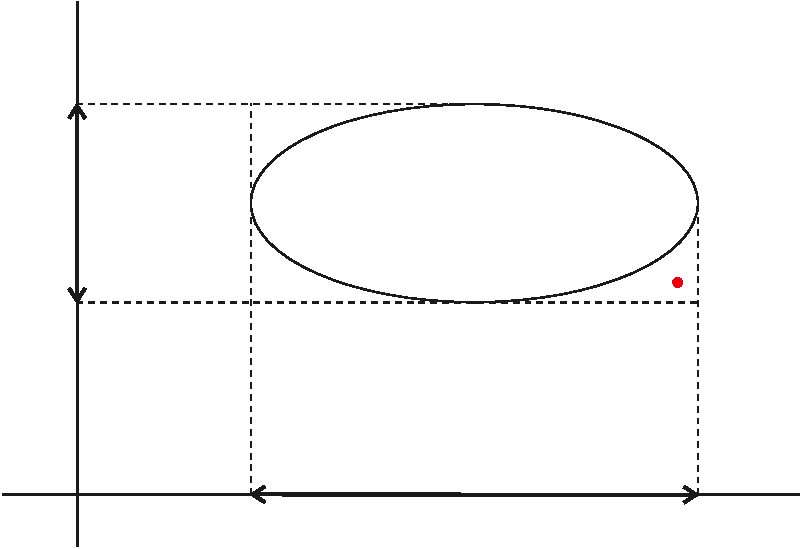
\includegraphics[width = 13cm]{pictures/picture_3_F.pdf}};
    \draw [color = red](5.0,0.0) node[anchor = north west] { $(x_{01},x_{02})$ };
    \draw [color = black](-5.9,4.2) node[anchor = north west] { $x_2$ };
    \draw [color = black](5.5,-3.7) node[anchor = north west] { $x_1$ };
     \draw [color = black](-1.0,1.4) node[anchor = north west] { $\text{společný obor dat } (x_1, x_2)$ };
     \draw [color = black](-0.0,-3.6) node[anchor = north west] { $\text{obor hodnot } x_1$ };
     \draw [color = black](-8.4,1.4) node[anchor = north west] { $\text{obor hodnot } x_2$ };
    \end{tikzpicture}
    \caption{ $(x_{01},x_{02})$ leží uvnitř oboru hodnot pro~obě $x_1$ i~$x_2$ ale vně společného oboru původních dat.}
\end{figure}
	\end{remark}
\end{example}

\chapter{Rezidua, diagnostika a~transformace}
\begin{itemize}
 \item Je třeba ověřit adekvátnost modelu. Máme $\RMR^2, \mathrm{t}, \text{F}$ statistiky, ty ale byly odvozeny za~předpokladu linearity modelu a~dalších podmínek na~náhodné chyby. Pro~ověření je důležitý nástroj analýza reziduí
 \item Je také třeba ověřit vliv jednotlivých pozorování na~model - analýza odlehlých (outliers) a~influenčních pozorování. (Velké reziduum pro~$i~$-té pozorování naznačuje problém s~modelem, ale může to být i~naopak, vlivné pozorování nemusí mít velké reziduum)
 \item Pokud detekujeme nějaké problémy s~modelem, mohou pomoci transformace proměnných nebo metoda na~korekci nekonstantního rozptylu.
\end{itemize}
\section{Rezidua}
připomenutí:
 $$
 \widehat{\textbf{y}} = \X \widehat{\beta} = \textbf{Hy}, \quad \text{kde} \quad \textbf{H} = \X (\X^T \X)^{-1} \X^T
 $$
 $$
 \widehat{\textbf{e}} = \textbf{y} - \widehat{\textbf{y}} = (\textbf{I}_n - \textbf{H}) \textbf{y} = (\textbf{I}_n - \textbf{H}) \textbf{e}
 $$
Dále jsme ukázali:
 $$
\E [\widehat{\textbf{e}}] = 0 \quad \text{Cov}(\widehat{\textbf{e}}) = \sigma^2 (\textbf{I}_n - \textbf{H})
 $$
Pokud navíc
 $
\textbf{e} \sim \text{N}_n (0,\sigma^2 \textbf{I}) $potom$ \widehat{\textbf{e}} \sim \text{N}_n (0,\sigma^2 (\textbf{I}_n - \textbf{H}))
 $. \\ Pokud označíme$ h_{ii} = \textbf{H}_{ii} $,$ \widehat{\textbf{e}}_i \sim \text{N} (0, \sigma^2 (1 - h_{ii}) $,$ \text{Cov}(\widehat{\textbf{e}}_i, \widehat{\textbf{e}}_j) = -\sigma^2 h_{ij} $. \\
Obecně bývá vhodnější pracovat se~standardizovanými rezidui, protože $\D [\widehat{\textbf{e}}_i] = \sigma^2 (1 - h_{ii})$, pro~$r_i = \frac{\widehat{\textbf{e}}_i}{\sigma \sqrt{1-h_{ii}}}$ platí $\D [r_i] = 1$.
 $\sigma$ odhadneme pomocí $s_n = \sqrt{\frac{1}{n-m-1} \SSE}$, dostaneme
 $$
  \widehat{r}_i = \frac{\widehat{\textbf{e}}_i}{s_n \sqrt{1 - h_{ii}}} \quad \text{kde} \quad i\in\widehat{n} \quad \text{(Interně studentizované reziduum)}
 $$
(Někdy také standardizovaná rezidua) \\
R : rstandard(.) \\
Pokud $\sigma^2$ odhadneme na~základě modelu, ve~kterém bylo vynecháno $i$-té pozorování, označíme tento odhad $\sigma^2_{(-i)}$, potom
 $$
 \widehat{\mathrm{t}}_i = \frac{\widehat{\textbf{e}}_i}{  \sigma^2_{(-i)} \sqrt{1 - h_{ii}}} \quad \text{kde} \quad i\in\widehat{n} \quad \text{(Externě studentizované reziduum)}
 $$
(Někdy také studentizované rezidua) \\
R : rstudent(.) \\
Například $\sigma^2_{(-i)} = \frac{\SSE_{(-i)}}{n-m-1}$ je nestranný odhad $\sigma^2$ v~modelu $(-i)$.

\begin{remark}
Platí:
\begin{itemize}
\item Pokud $h_{ii}$ je malé, pro~velké $n$ by se~mělo $\widehat{\text{e}}_i, \widehat{\text{r}}_i, \widehat{\mathrm{t}}_i$ chovat přibližně stejně a~$\widehat{\text{r}}_i,\widehat{\mathrm{t}}_i \approx \text{N} (0, 1)$.
\item Pro~malé $n$$ (n < 20) $a~/ nebo$ h_{ii} \approx 1 $je preferováno použít$ \widehat{\text{r}}_i $nebo$ \widehat{\mathrm{t}}_i $a~aktuálně bývá častěji doporučována$ \widehat{\mathrm{t}}_i $($ i~$-té pozorování s~velkými$ h_{ii} $může zvyšovat odhad$ \sigma^2 $ a~tím snižuje velikost svého rezidua).
\item $h_{ii}$ hraje zásadní roli v~diagnostice modelu, probereme teď jeho základní vlastnosti.
\end{itemize}
\end{remark}

\textbf{Leverage} $h_{ii}$ - potenciál $i$-tého pozorování (leverage point - píkový bod / vzdálený bod)

\begin{itemize}
\item $\D [\widehat{\text{e}}_i] = \sigma^2 (1 - h_{ii}) \geq 0 \Rightarrow h_{ii} \leq 1$.
\item $\textbf{H}^2 = \textbf{H} \Rightarrow h_{ii} = \sumjn h_{ij} h_{ji} = \sumjn (h_{ij})^2$ tedy $h_{ii} > 0$ (Dá se~ukázat silnější tvrzení: $h_{ii} \geq \frac{1}{n}$).
\item $\textbf{H}^2 = \textbf{H} \Rightarrow \textbf{A}_{i1} = \sumjn h_{ij} x_{j1} = \sumjn h_{ij} = x_{i1} = 1$ tedy
 $$ \sumjn h_{ij} = 1 \quad \forall j \in \widehat{n} $$.
\item Význam $h_{ii}$ vyplyne z~následujících úvahy:
 $$
 \widehat{\textbf{y}} = \textbf{Hy} \Rightarrow \widehat{y}_i = \sumjn h_{ij}y_j = h_{ii} y_i + \sum\limits_{\substack{j = 1 \\ i\neq j}}^n h_{ij} y_j
 $$
, pokud $h_{ii} \approx 1$, potom $\widehat{y}_i \approx y_i$ a~model je nucen proložit přímku bodem ($\textbf{x}_i, y_i$), i~když když tam neplatí body s~"velkým $h_{ii}$ " - body s~velkým potenciálem (high leverage points). Tyto body by měly být detekovány pro~další zkoumání.
 \item Otázka je, jaká hodnota $h_{ii}$ je "velká".
\end{itemize}
\textbf{Heuristické pravidlo:}
 $\sum_{i = 1}^n h_{ii} = \text{tr}(\textbf{H}) = m + 1$, tzn. $\frac{m+1}{n}$ je průměrná hodnota $h_{ii}$. $i$-té pozorování má velký potenciál jestliže $h_{ii} > \frac{3(m+1)}{n}$. (Stejně postupuje i~jazyk R)

\section{Grafy reziduí}
\begin{enumerate}
\item Ověření normality - histogramy, Q-Q plots \\
tyto obrázky nezávisí na~počtu nezávislých proměnných $x$, vše stejné jako v~jednoduché LR.
\item Pro~ověření funkční formy pro~$\E [Y_x]$ a~/ nebo konstantního rozptylu se~nejčastěji používají:
\begin{enumerate}
\item Grafy $\widehat{e}_i, \widehat{r}_i$ nebo $\widehat{t}_i$ oproti~$\textbf{x}_j^c$, $j = 1,..., m$, kde $\textbf{x}_j^c$ je $j$-tý sloupec $\X$
\item  Grafy $\widehat{e}_i, \widehat{r}_i$ nebo $\widehat{t}_i$ oproti~$\widehat{y}_i$
\item Partial residual plots
\end{enumerate}
\end{enumerate}

\begin{remark}
Zdůvodnění:
\begin{enumerate}
\item Normální rovnice $\X^T (\textbf{y} - \X \widehat{\beta}) = 0$ implikují $\X^T (\textbf{y} - \widehat{\textbf{y}}) = \X^T \widehat{\textbf{e}}$.
 $$
 \text{Připomenutí:} \quad \text{Y}_i = \beta_1 x_i + e_i, \quad \widehat{\beta}_1 = \frac{\sum_{i = 1}^n x_i y_i}{\sum_{i = 1}^n x_i^2} = \frac{\textbf{x}^T\textbf{y}}{| \textbf{x} |^2 }
 $$
Pokud tedy naladíme LR model bez~interceptu pro~$\widehat{\textbf{e}}$ v~závislosti na~$\textbf{x}_j^c$, směrnice přímky bude
 $$
  \widehat{\beta}_j^* = \frac{(\textbf{x}_j^c)^T \widehat{\textbf{e}}}{| \textbf{x}_j^c |^2} = 0
 $$
Graf $\widehat{e}_i, \widehat{r}_i, \widehat{t}_i$ oproti~$\textbf{x}_j^c$ by měl dávat náhodně rozptýlené body kolem~osy $x$. (bez trendů, $\widehat{r}_i, \widehat{t}_i$ uvnitř ???? $\pm 2$)
Pokud tomu tak není, může to naznačovat nelinearitu v~$\textbf{x}_j$ nebo nekonstantní rozptyl.
\item Ukázali jsme $\sum_{i = 1}^n \widehat{y}_i \widehat{e}_i = 0$ pro~LM bez~interceptu pro~$\widehat{e}_i$ oproti~$\widehat{y}_i$ tedy platí
 $$
  \widehat{\beta} = \frac{\widehat{\textbf{e}}^T \widehat{\textbf{y}}}{| \widehat{\textbf{y}} |^2} = 0
 $$
Body by opět měly být náhodně rozptýlené kolem~osy $x$
\begin{itemize}
\item Trychtýřovitý tvar indikuje nekonstantní rozptyl.
\item Trendy indikují nelinearitu.
\end{itemize}
\end{enumerate}	
\end{remark}

\subsection{Partial residual plot}
\begin{itemize}
\item, i~když grafy $\widehat{e}_i$ oproti~$\textbf{x}_j^c$ a~$\widehat{\textbf{y}}$ mohou indukovat nedostatky modelu, nemusí být zřejmé, jaké ty nedostatky jsou.
\item V~SLR graf $\widehat{e}_i$ oproti~$x_i$ lze použít pro~detekci nelinearity
\item Ale v~MLR tyto grafy, stejně jako scatterploty, mohou být zavádějící, protože $\widehat{\textbf{e}}$ závisí na~všech prediktorech, nemusí být tedy izolován efekt dané proměnné při~odstranění efektů ostatních.
\item Pro~zkoumané efekty $j$-té proměnné lze použít partial rezidual plots - lze je chápat jako jeho ekvivalent scatterplotu v~SLR

\begin{define}
 $$
   \widehat{e}_j^* = \widehat{\textbf{e}} + \widehat{\beta}_j \textbf{x}_j^c,
 $$
 kde $\widehat{\textbf{e}}$ je vektor reziduí modelu, $\widehat{\beta}_j$ je LSE parametru $\beta_j$, $\textbf{x}_j^c$ je $j$-tý sloupec $\X$
\end{define}
\end{itemize}
Partial residual plot (PRP): graf $\widehat{\textbf{e}}$ oproti~$\textbf{x}_j^c$, $j = 1,..., m$, pokud je model správný, měly by být body náhodně rozmístěné kolem~přímky se~směrnicí $\widehat{\beta}_j$.

\textbf{Zdůvodnění}: Vztah mezi~$\heb_j^*$ a~$\x_j^c$ má formu SLR bez~interceptu, pokud je model správný, $\hei, i\in\widehat{n} $, splňují podmínku $\E \hei = 0$ a~$\D \hei = \sigma^2(1 - h_{neco})$. Má tedy smysl uvažovat RM pro~$\heb_j^*$ oproti~$\x_j^c$ ($\he_j^* = \gamma_j \x_j^c + \eb$).

\newcommand{\hg}{\widehat{\gamma}}

Pro odhad koeficientů platí, že
 $$
\hg_j = \frac{(\heb_j^* \x_j^c)}{\norm{\x_j^c}^2} = \frac{(\heb + \wbeta_j \x_j^c)^T \x_j^c}{\norm{\x_j^c}^2} = \frac{\heb^T \x_j^c + \wbeta_j \norm{\x_j^c}^2}{\norm{\x_j^c}^2} = \wbeta_j,
 $$
protože $\heb^T \x_j^c = 0$.

(2 příklady - pdf 79-93 uprostřed str 6)

\newcommand{\wb}{\mathbf{w}}
\newcommand{\identita}{\mathbb{I}}
\newcommand{\Xmj}{\X_{(-j)}}
\newcommand{\Xmi}{\X_{(-i)}}

\begin{remark}
	PRPs jsou někdy kritizovány za~nadhodnocování efektu $\x_j^c$. \linebreak
	Alternativa: \textbf{partial regression plot (added variable plot)}. \linebreak
	Motivace: Ptáme se, zda přidat novou proměnnou do~modelu a~chtěli bychom dohadnout její efekt.
	
	Budeme tedy uvažovat rozšířený model
	 $$
	\Y = \X \betab + \gamma \wb + \eb,
	 $$
	kde $\wb$ je nový vektor regresorů. Model lze rozepsat jako
	 $$
	\Y = \begin{bmatrix}
	\X \wb
	\end{bmatrix} \begin{pmatrix}
	\betab \\ \gamma
	\end{pmatrix} + \eb = \X_w + \betab_w + \eb.
	 $$
	Použitím normálních rovnic pro~$\X_w$ lze odvodit formuli pro~$\hg$
	\begin{equation*}
		\hg = \frac{\heb^T (\identita - \Hm) \wb}{\norm{(\identita - \Hm)\wb}^2}.
		\tag{\#}
		\label{Eq: hat gamma}
	\end{equation*}
	 $\hg$ je směrnice RM pro~$\heb$ v~závislosti na~$\wb_{res} = (\identita - \Hm)\wb$ (rezidua modelu pro~$\wb$ v~závislosti na~$\X$).
	
	Teď naopak uvažujme, že $\wb$ je sloupec původní $\X$, řekněme $\x_j^c$ a~ozn. $\Xmj$ matici $\X$ bez~sloupce $j$. V~předchozím modelu pomožme $\X = \Xmj$ a~$\wb = \x_j^c$. Potom  LSE $\wbeta_j$ parametru $\beta_j$ je
	 $$
	\wbeta_j = \frac{\heb_{(-j)}^T \x_{j, res}^c}{\norm{\x_{j,res}^c}^2},
	 $$
	kde $\heb_{(-j)}$ jsou rezidua modelu bez~$\x_j^c$, $\x_{j,res}^c = (\identita - \Hm) \x_j^c$, tedy jsou to rezidua modelu pro~$\x_j^c$ v~závislosti na~ostatních proměnných, tedy $\Xmj$ (v $\x_{j,res}^c$ je tedy odstraněn efekt ostatních regresorů).
	
	 $\wbeta_j$ je směrnice RM pro~$\heb_{(-j)}$ v~závislosti na~$\x_{j, res} \Rightarrow$ \linebreak
	\textbf{added variable plot}: graf $\heb_{(-j)}$ proti~$\x_{j, res}, j = 1,..., m$.
	
	Pokud je model správný, body by měly být náhodně rozptýlené kolem~přímky se~směrnicí $\wbeta_j$ procházející počátkem. Pokud závislost na~$\x_j^c$ není lineární, projeví se~to odklonem bodů od~přímky.
\end{remark}

\begin{remark}
Ze vztahu \eqref{Eq: hat gamma} je vidět, že MLR může být chápána jako posloupnost SLR, kde postupně vytváříme modely pro~novou proměnnou s~použitím reziduí modelu pro~předcházející proměnné.
\end{remark}

\section{PRESS rezidua (PRESS residuals, deleted residuals)}
\begin{itemize}
	\item, pokud budeme chtít model použít nejen k~vysvětlení vztahu mezi~proměnnými, ale také pro~predikci, hodila by se~míra vyjadřující jak dobře model predikuje (doposud jsme zkoumali jen jak dobře popisuje)
	\item šlo by použít IS nebo IP, to bychom ale předem museli znát body, ve~kterých chceme predikovat
	\item nejjednodušší přístup, jak měřit prediktivní přesnost modelu by byl analýza reziduí pro~predikce hodnot v~nových bodech $\x$, obecně ale nemáme data $y$ v~těchto bodech
	\item jedna možnost je použít data, která máme k~dispozici
\end{itemize}

\textbf{Postup}: Vynecháme jedno pozorování, naladíme model bez~tohoto pozorování a~porovnáme predikovanou a~pozorovanou hodnotu pro~vynechané pozorování.

Předpokládáme, že vynecháme $i$-té pozorování. Ozn. $\wbetab_{(-i)}$ odhad $\betab$ v~modelu s~vynechaným $i$-tým pozorováním (M $_{-i}$) a~$\hy_{(-i)}$ predikovanou hodnotu modelem M $_{(-i)}$ v~bodě $\x_i^T$, tzn. $\hy_{(-i)} = \x_i^T \wbetab_{(-i)}$.

Potom
 $$
\heb_{(-i)} = y_i - \hy_{(-i)}, \quad i\in\widehat{n}
 $$
nazýváme $i$-té \textbf{PRESS reziduum}.

 $\mathrm{PRESS} = \sum_{i = 1}^n \he_{-i}^2$ je užitečná míra přesnosti predikce.

\begin{remark}
	Otázka je, jak počítat $\he_{(-i)}, i\in\widehat{n} $.
	\begin{itemize}
		\item pro~velké $n$ se~zdá, že to bude náročný problém, protože pro~každé $i \in \widehat{n}$ musíme naladit nový model
		\item naštěstí to není nutné, ukážeme totiž, že
		 $$
		\he_{(-i)} = \frac{\he_i}{1 - \hii},
		 $$
		tzn. všechna $\he_{(-i)}$ lze snadno spočítat pomocí reziduí a~hodnot $\hii$ z~původního (plného) modelu.
	\end{itemize}
\end{remark}

Označme
\begin{align*}
	\x_i^T & \text{ - $i$-tý řádek matice } \X \\
	\Xmi & \text{ - matici $\X$ bez~$i$-tého řádku}
\end{align*}

\newcommand{\XtX}{\left(\X^T \X \right)^{-1}}

\begin{theorem}
Jestliže $\hii \neq 1$, potom
 $$
\left[\Xmi^T \Xmi \right] = \X^T \inv{\X} + \frac{\XtX \x_i \x_i^T \XtX}{1 - \hii},
 $$
kde $\hii$ je $i$-tý diagonální prvek matice $\Hm$.
\end{theorem}

\begin{proof}
Nejdříve ukážeme
\begin{equation*}
	\X^T \X = \Xmi^T \Xmi + \x_i \x_i^T \tag{+} \label{Eq: plus}
	%(m+1) \times (m+1) & (m+1) \times (m+1) & (m+1) \times (m+1)
\end{equation*}

\newcommand{\sumkn}{\sum_{k = 1}^n}
\newcommand{\sumknn}{\sum_{k = 1}^{n-1}}

Kvůli značení předpokládáme $i = n$ (toho se~dá vždy dosáhnout permutací řádků $\X$). Potom
 $$
\left(\X^T \X \right)_{ij} = \sumkn x_{ki} x_{kj} = \sumknn x_{ki} x_{kj} + x_{ni} x_{nj}.
 $$
 $i,j$-tý prvek $\X_{(-k)}^T \X_{(-k)}$ je $\sumknn x_{ki} x_{kj}$ \\
 $i,j$-tý prvek $\x_n \x_n^T$ je $x_{ni} x_{nj}$, tzn. \eqref{Eq: plus} platí.



\begin{theorem}[Sherman-Morrison-Woodburry (z LA)]
Nechť $\Am$ je $n \times n$ invertibilní matice a~nechť $\z$ je $n \times 1$ sloupcový vektor. Jestliže $\z^T \inv{\Am} \z \neq 1$, potom matice $\Bm = \Am - \z^T \z$ je invertibilní a~platí
 $$
\inv{\Bm} = \inv{\Am} + \frac{\inv{\Am} \z^T \z \inv{\Am}}{1 - \z^T \inv{\Am} \z}.
 $$
\end{theorem}

Položme $\Am = \X^T \X$, $\z = \x_i$, $\Bm = \X_{(-i)}^T \X_{(-i)}$. Pak $\Bm = \Am - \z \z^T$, $\Am$ je invertibilní a
 $$
\z^T \inv{\Am} \z = \x_i^T \XtX \x_i = \left(\X \XtX \X^T \right)_{ii} = \hii \neq 1.
 $$
Užitím věty dostaneme
 $$
\left(\X_{(-i)}^T \X_{(-i)} \right)^{-1} = \XtX + \frac{\XtX \x_i \x_i^T \XtX}{1 - \hii}.
 $$

\end{proof}

\begin{theorem}
	Nechť $\he_{(-i)}$ je $i$-té PRESS reziduum. Potom
	 $$
	\he_{(-i)} = \frac{\he_i}{1 - \hii}, \quad i\in\widehat{n}.
	 $$
\end{theorem}

\begin{proof}
	
	Nechť $\wbetab_{(-i)}$ je odhad $\betab$ v~modelu M $_{-i}$, tzn.
	 $$
	\wbetab_{(-i)} = \left(\X_{(-i)}^T \X_{(-i)} \right)^{-1} \X_{(-i)}^T \y_{(-i)},
	 $$
	tedy $\y_{(-i)}$ je $\y$ bez~$i$-té složky $y_i$. To znamená, že
	\begin{align*}
	\hy_{(-i)} & = \x_i^T \wbetab_{(-i)} = \x_i^T \inv{\left(\X_{(-i)}^T \X_{(-i)} \right)} \X_{(-i)}^T \y_{(-i)} = \\
	 & = \left[\left(\X_{(-i)}^T \X_{(-i)} \right)^{-1} = \XtX + \frac{\XtX \x_i \x_i^T \XtX}{1 - \hii}. \right] = \\
	 & = \x_i^T \XtX \X_{(-i)}^T \y_{(-i)} + \frac{1}{1 - \hii} \x_i^T \XtX \x_i \x_i^T \XtX \X_{(-i)}^T \y_{(-i)} = \\
	 & = S_1 + \frac{1}{1-\hii} S_2.
	\end{align*}
	
	Protože $\X_{(-i)}^T \y_{(-i)} = \X^T \y - y_i \x_i$, dostaneme
	\begin{align*}
	S_1 & = \x_i \XtX \left(\X^T \y - y_i \x_i \right) = \x_i^T \underbrace{\XtX \X^T \y}_{\wbetab} - y_i \underbrace{\x_i^T \XtX \x_i}_{\hii} = \\
	& = \x_i^T \wbetab - \hii y_i = \hy_i - \hii y_i.
	\end{align*}
	Podobně	
	 $$ S_2 = \underbrace{\textbf{x}_i^T(\textbf{x}^T\textbf{x})^{-1}\textbf{x}_i}_{h_{ii}}\underbrace{\textbf{x}_i^T(\textbf{x}^T\textbf{x})^{-1}\textbf{x}\textbf{y}}_{\hyi} = y_i\underbrace{\textbf{x}_i^T(\textbf{x}^T\textbf{x})^{-1}\textbf{x}_i}_{h_{ii}}\underbrace{\textbf{x}_i^T(\textbf{x}^T\textbf{x})^{-1}\textbf{x}_i}_{h_{ii}} = h_{ii}\hyi-y_ih_{ii}^2 $$
	takže
	 $$ \hy_{(-i)} = \hyi-h_{ii}y_i+\frac{1}{1-h_{ii}}(h_{ii}\hyi-y_ih_{ii}^2). $$
	Celkem tedy
	\begin{align*}
	\he_{-i} & = y_i-\hy_{(-i)} = y_i(1+h_{ii})-\hyi-\frac{1}{1-h_{ii}}(h_{ii}\hyi-y_ih_{ii}^2) = \\
	& = \frac{1}{1-h_{ii}}\big(y_i(1-h_{ii}^2)-\hyi(1-h_{ii})-h_{ii}\hyi+y_ih_{ii}^2\big) = \frac{1}{1-h_{ii}}(y_i-\hyi) = \frac{\hei}{1-h_{ii}}
	\end{align*}
\end{proof}Budeme potřebovat podobné formule pro~$\wbetab-\wbetab_{(-1)}$ a~$\mini{\SSE}$.

\begin{theorem}
	\begin{enumerate}[1)]
		\item Nechť $\mini{\wbetab}$ značí $\LSE$ parametru $\wbetab$ v~modelu bez~$i$-tého pozorování. Potom platí
	 $$ \wbetab-\mini{\wbetab} = \frac{(\textbf{X}^T\textbf{X})^{-1}\textbf{x}_i\hei}{1-\hii} = (\textbf{X}^T\textbf{X})^{-1}\textbf{x}_i\mini{\he}. $$
	\item Pro~součet residuálních čtverců $\mini{\SSE}$ v~modelu bez~$i$-tého pozorování platí
	 $$ \mini{\SSE} = \sumjn \he_j^2-\frac{\he_i^2}{1-\hii}. $$
	\end{enumerate}

\begin{proof}
	\begin{enumerate}[1)]
		\item Stejně jako v~důkazu předchozí věty platí, že
		 $$ \mini{\wbetab} = S_1+\frac{1}{1-\hii}S_2, $$
		kde $S_1 = \wbetab-y_i\inv{(\textbf{X}^T\textbf{X})}\textbf{x}_i$ a~$S_2 = \inv{\textbf{X}^T\textbf{X}}\textbf{x}_i\hyi-y_i\core \textbf{x}_i\hii$, tedy
		\[
		\begin{split}
		\wbetab-\mini{\wbetab}& = y_i\core\textbf{x}_i-\frac{1}{1-\hii}\big(\core x_i\hyi-y_i\core \textbf{x}_i\hii\big) = \\& = \core \textbf{x}_i\Big(y_i-\frac{\hyi-y_i\hii}{1-\hii}\Big) = \core \textbf{x}_i\Big(\frac{y_i-y_i\hii-\hyi+y_i\hii}{1-\hii}\Big) = \\& = \core \textbf{x}_i\Big(\frac{y_i-\hyi}{1-\hii}\Big),
		\end{split}
		\]
		kde $\Big(\frac{y_i-\hyi}{1-\hii}\Big) = \frac{\hei}{1-\hii} = \mini{\he}$.
		\item \[
		\begin{split}
		\mini{\SSE}& = \big(\mini{\textbf{y}}-\mini{\textbf{x}}^T\mini{\wbetab}\big)^T\big(\mini{\textbf{y}}-\mini{\textbf{x}}^T\mini{\wbetab}\big) = \sum_{\substack{j = 1\\j\neq i}}^n(y_j-\textbf{x}_j^T\mini{\wbetab})^2 = \\& = \sumjn (y_j-\textbf{x}_j^T\mini{\wbetab})^2-(y_i-\textbf{x}_i^T\mini{\wbetab})^2.
		\end{split}
		\]
		Z bodu 1) víme, že $\mini{\wbetab} = \wbetab-\frac{\core \textbf{x}_i\hei}{1-\hii}$, tzn.
		 $$ \mini{\SSE} = \sumjn\Big(y_j-\textbf{x}_j^T\wbetab+\frac{\textbf{x}_j^T\core \textbf{x}_i\hei}{1-\hii}\Big)^2-\Big(y_i-\textbf{x}_i^T\wbetab+\frac{\textbf{x}_i^T\core \textbf{x}_i\hei}{1-\hii}\Big)^2. $$
		Protože $\textbf{x}_j^T\core \textbf{x}_i = h_{ij}$, dostaneme
		\[
	\begin{split}
	\mini{\SSE}& = \sumjn \Big(\he_j+\frac{h_{ij}\hei}{1-\hii}\Big)^2-\Big(\he_i+\frac{h_{ii}\hei}{1-\hii}\Big)^2 = \underbrace{\sumjn\Big(\he_j+\frac{h_{ij}\hei}{1-\hii}\Big)^2}_A-\frac{\hei^2}{(1-\hii)^2},\\
	A& = \sumjn \he_j^2+\frac{2\hei}{1-\hii}\underbrace{\sumjn h_{ij}\he_j}_0+\frac{\hei^2}{(1-\hii)^2}\underbrace{\sumjn h_{ij}^2}_{\hii}.
	\end{split}
	\]
		Protože pak $\hyb = \textbf{H}\textbf{y}$, tak $\textbf{H}\hyb = \textbf{H}^2\textbf{y} = \textbf{H}\textbf{y}$, a~tedy $\textbf{H}\heb = \textbf{H}(\textbf{y}-\hyb) = \textbf{H}\textbf{y}-\textbf{H}\hyb = 0$, a~tedy
		 $$ \mini{\SSE} = \sumjn\he_j^2+\frac{\hei^2}{(1-\hii)^2}(\hii-1) = \sumjn\he_j^2-\frac{\hei^2}{1-\hii}. $$
	\end{enumerate}
\end{proof}
\end{theorem}

\begin{dusl}
	V modelu (**) s~$m+1$ parametry $\beta$ a~bez~$i$-tého pozorování platí, že $$ \EE{\mini{\SSE}} = (n-m-2)\sigma^2, $$
	takže
	 $$ \mini{\widehat{{\sigma}^2}} = \frac{\mini{\SSE}}{n-m-2} $$ je nestranný odhad $\sigma^2$. Dále pak
	 $$ \mini{\widehat{{\sigma}^2}} = \frac{(1-\hii)(n-m-1)s_n^2-\hei^2}{(1-\hii)(n-m-2)} = \frac{1}{n-m-2}\Big(\SSE -\frac{\hei^2}{1-\hii}\Big), $$ kde $s_n^2 = \frac{1}{n-m-1}\SSE$ (pro plný model).
	\begin{proof}
		Protože $\EE{\hei^2} = \D \hei = \sigma^2(1-\hii)$, dostaneme dle předchozí věty
		\[
		\begin{split}
		&\EE{\mini{\SSE}} = \sumjn\sigma^2(1-h_{jj})-\sigma^2 = \sigma^2\big[(n-1)-\underbrace{\sumjn h_{jj}}_{h\textbf{H = m+1}}\big] = \sigma^2(n-m-2)\\
		&\mini{\widehat{{\sigma}^2}} = \frac{1}{n-m-2}\mini{\SSE} = \frac{1}{n-m-2}\Big(\underbrace{\sumjn\he_j^2}_{\SSE = (n-m-1)s_n^2}-\frac{\hei^2}{1-\hii}\Big) = \frac{1}{n-m-2}\frac{(1-\hii)\SSE-\hei^2}{1-\hii}.
		\end{split}
		\]
	\end{proof}
\end{dusl}

\begin{remark}
	Dě se~ukázat, že $\mini{\SSE}$ a~$\hei$ jsou nezávislé náhodné veličiny. Protože $\frac{\mini{\SSE}}{\sigma^2}\sim\chi^2(n-m-2)$ a~$\frac{\hei}{\sigma\sqrt{1-\hii}}\sim\NN(0,1)$, dostaneme $\frac{\hei}{\mini{\widehat{{\sigma}^2}}\sqrt{1-\hii}}\sim t(n-m-2)$.
\end{remark}

\begin{corollary}
	Uvažujme model (**), kde $h(X) = m+1$ a~$\textbf{e}\sim\NN_m(0,\sigma^2 I_m)$. Nechť pro~$i\in\widehat{n}$ platí, že $\hii\neq1$. Potom $i$-té ??????????91dole? reziduum
	 $$ \widehat{t}_i\sim t(n-m-2). $$
\end{corollary}
\begin{remark}
	 $\widehat{t}_i$ lze použít pro~test hypotézy, zda je $i$-té pozorování odlehlé (outlier), tedy
	\[
	\begin{split}
	&H_0:~i\text{-té pozorování není odlehlé v~modelu }M\\
	&H_1:~i\text{-té pozorování je odlehlé v~}M,
	\end{split}
	\] kde odlehlé značí odlehlé vzhledem k~$M:~\textbf{Y}\sim\NN_m(\textbf{X}\beta,\sigma^2 I_m)$ :\begin{enumerate}[a)]
		\item střední hodnota $i$-tého pozorování se~nerovná té dané modelem,
		\item pozorovaná hodnota $Y_i$ je neobvyklá za~platnosti $M$.
	\end{enumerate}
 $H_0$ zamítneme, pokud $$ |\widehat{t}_i|>t_{1-\frac{\alpha}{2}}(n-m-2)\approx u_{1-\frac{\lparen}{2}}\doteq 2\text{ pro~}\alpha = 0.05\text{ a~}n\text{ velká}. $$
Pokud test použijeme na~všechna pozorování, je potřeba aplikovat nějakou korekci na~vícenásobné testování, např. Bonferroni.
\end{remark}
\begin{remark}
	Vztah $\mini{\he}$ a~$\widehat{t}_i$ :
	 $$ \mini{\he} = \frac{\hei}{1-\hii}\quad\Rightarrow\quad\E\mini{\he} = 0\quad\wedge\quad \D \mini{\he} = \frac{\sigma^2}{1-\hii}. $$
	Standardizované PRESS reziduum $$ \frac{\mini{\he}}{\sqrt{D\mini{\he}}} = \frac{\frac{\hei}{1-\hii}}{\frac{\sigma}{\sqrt{1-\hii}}} = \frac{\hei}{\sigma\sqrt{1-\hii}} = r_i. $$
	Pokud použijeme $\mini{\widehat{{\sigma}^2}}$ jako odhad $\sigma^2$, pak \textbf{studentizovaná PRESS rezidua} $$ \frac{\hei}{\mini{\widehat{{\sigma}}}\sqrt{1-\hii}} = \widehat{t}_i. $$
\end{remark}
\begin{remark}
	 $\mini{\he} = \frac{\hei}{1-\hii}$, a~proto, pokud $i$-té pozorování má velký potenciál $\hii$, bude $\mini{\he}$ mnohem větší, než $\hei$, pozorování s~velkým $\hii$ jsou dobře modelována, ale měřeno $\mini{\he}$ mohou špatně predikovat. To je další ukázka fit/prediction dilema.
	
	Stejný efekt nastává také pro~
	 $$ \wbetab_i-\mini{\wbetab} = \core\textbf{x}_i\mini{\he}. $$
	Rozdíl může být "malý", pokud je "fit" dobrý, ale může být také "velký", pokud je $\hii$ velké.
\end{remark}

\section{Míry influence}
\begin{itemize}
	\item I~pro~perfektní model mohou dva různé vzorky $(\textbf{x},\textbf{y})$ a~$(\textbf{x}',\textbf{y}')$ vést k~různým závěrům,
	\item většinou máme k~dispozici jen originální data,
	\item bude nás zajímat vliv $i$-tého řádku $\textbf{x}$ na~model,
	\item už víme, že velké $\hii$ indikuje, že $i$-té pozorování má velký vliv a~velká rezidua naznačují možnou neadekvátnost modelu,
	\item míry, které zavedeme, budou kombinovat tyto dva faktory,
	\item použijeme přístup z~PRESS residní, tzn. budeme sledovat jak velký vliv má vynechání $i$-tého pozorování na~$\wbetab$ a~$\widehat{\textbf{y}}$.
\end{itemize}
\subsection*{DFBETAS}
 $\wbetab-\mini{\wbetab}$ měří vliv vynechání $i$-tého pozorování na~odhad $\wbeta$ (bude základem pro~naši analýzu). Připomeňme nyní vztah
 $$ \wbetab-\mini{\wbetab} = \core \textbf{x}_i\frac{\hei}{1-\hii}. $$

\begin{description}
	\item[a) vliv $i$-tého pozorování na~$\beta_j$ :]
	 $$ \beta_j-\mini{\beta}{}_j = \frac{r_{ij}\hei}{1-\hii},\quad\text{ kde }r_{ji}\text{ je }(j,i)\text{tý prvek matice }\R = \core\textbf{x}^T. $$
	
	 $i$-té pozorování budeme považovat za~influenční na~$\beta_j$, pokud $\wbeta_j-\mini{\wbeta}{}_j$ bude velká. Protože $\wbeta _j$ je náhodná veličina, "velké" bychom měli měřit relativně vzhledem k~s.f. $(\wbeta _j$, což je $\sigma\sqrt{v_j}$, $v_j = \core _{jj})$. Pokud ji odhadneme pomocí $\mini{\widehat{{\sigma}}}\sqrt{v_j}$, dostaneme definici
	 $$ \mathrm{DFBETAS}_{j,i} = \frac{\wbeta_j-\mini{\wbeta}{}_j}{\mini{\widehat{{\sigma}}}\sqrt{v_j}} = \frac{r_{ji}\hei}{\sqrt{v_j}\mini{\widehat{{\sigma}}}(1-\hii)} = \frac{r_{ji}}{\sqrt{v_j}}\frac{\widehat{t}_i}{\sqrt{1-\hii}}, $$
	kde $\widehat{t}_i$ je ext. studentizované reziduum. Kombinuje efekt velkého rezidua $\widehat{t}_i$ a~velkého $\hii$. Jedna možnost pro~limitní hodnoty: $i$-té pozorování je považováno za~influenční na~oblasti $\beta_j$, pokud
	 $$ |\mathrm{DFBETAS}_{j,i}|>\frac{2}{\sqrt{n}}. $$ Máme $(m+1)\times n$ hodnot pro~srovnání, zjednodušíme to.
	\item[b) Vliv $i$-tého pozorování na~celý vektor $\wbetab$ :]
	spočívá v~použití nejaké normy na~vektor $\wbetab-\mini{\wbetab}$. Cook navrhnul
	 $$ D_i = \frac{(\wbetab-\mini{\wbetab})^T\textbf{M}(\wbetab-\mini{\wbetab})}{(m+1)c}, $$
	kde $\textbf{M}$ je PD matice a~$c$ normalizační konstanta. Nejužívanější volba je $\textbf{M} = \textbf{X}^T\textbf{X}$ a~$x = s_n^2$. Cookova vzdálenost se~potom spočítá jako
	 $$ D_i = \frac{(\wbetab-\mini{\wbetab})^T\textbf{X}^T\textbf{X}(\wbetab-\mini{\wbetab})}{(m+1)s_n^2}. $$
	
	 $$ D_i = \frac{1}{(m+1)s_n^2}\Big(\frac{\hei}{1-\hii}\Big)^2 \underbrace{\textbf{x}_i^T\core \underbrace{\textbf{x}^T\textbf{x}\core}_I\textbf{x}_i}_{\hii} = \frac{1}{m+1}\frac{\hii}{1-\hii}\frac{\hei^2}{s_n^2(1-\hii)}. $$
	Výpočetní formule je potom ve~tvaru
	 $$ D_i = \frac{\widehat{r}_i^2}{m+1}\Big(\frac{\hii}{1-\hii}\Big). $$
\end{description}

\begin{remark}
	 $100(1-\alpha)\%$ simultání IS pro~$\betab$ je $$ C(\alpha) = \Big\{ ~\betab~\Big|\frac{(\wbeta-\beta)^T\textbf{x}^T\textbf{x}(\wbeta-\beta)}{(m+1)s_n^2}\leq \FF_{1-\alpha}(m+1,n-m-1) \Big\}, $$
	tzn. $$ \mini{\betab}\in C(\alpha)\quad \Leftrightarrow\quad D_i\leq \FF_{1-\alpha}(m+1,n-m-1). $$
	To je motivace pro~\textbf{RULE OF THUMB}: $$ \text{ $i$-té pozorování je influenční, jestliže $D_i>\FF_{\frac{1}{2}}(m+1,n-m-1)$ } $$ (pro většinu $m,n$ je $\FF_{\frac{1}{2}}\approx1$, zjednodušení pravidla $D_i>1$).
\end{remark}

\begin{remark}
	Také platí, že
	 $$ D_i = \frac{(\widehat{\textbf{y}}-\mini{\widehat{\textbf{y}}})^T(\widehat{\textbf{y}}-\mini{\widehat{\textbf{y}}})}{(m+1)s_n^2}, $$
	tzn. dá se~chápat jako míra influence na~celkovou predikci.
\end{remark}

\subsection*{DFFITS}
\begin{itemize}
	\item vliv $i$-tého pozorování na~$\hy_i$
\end{itemize}
 $$ \mathrm{DFFITS}_i = \frac{\hyi-\mini{\hy}}{\mini{\widehat{{\sigma}}}\sqrt{\hii}} = ... = \widehat{t}_i\sqrt{\frac{\hii}{1-\hii}}. $$
RULE OF THUMB: $i$-té pozorování je influenční, pokud $|\mathrm{DFFITS}|>3\sqrt{\frac{m+1}{n-m-1}}$.

\begin{remark}[Míry influence v~R]
\begin{itemize}
	\item DFBETAS - \verb|dfbetas()|
	\item DFFITS - \verb|dffits()|
	\item Cookova vzdálenost $D_i$ - \verb|cooks.distance()|
	\item Leverage $\hii$ - \verb|hotvalues()|
	\item a~vše shrnuje funkce \verb|influence.measures()| (má navíc covariance ratio)
\end{itemize}

Používané pravidlo: $i$-té pozorování je influenční, pokud:
\begin{align*}
	& = | \mathrm{DFBETAS} | > 1, \quad |\mathrm{DFFITS}| > 3 \sqrt{\frac{m+1}{n-m-1}} \\
	& D_i > F_{0,5}(m+1,n-m-1), \quad \hii > 3 \frac{m+1}{n}
\end{align*}
\end{remark}

\section{Transformace}

Pokud není splněný ně, který z~předpokladů modelu: linearita, normalita chyb, homoskedasticita, jednou z~možností je pokusit se~transformovat nějaké proměnné, aby transformovaný model tyto předpoklady alespoň \uv{přibližně} splňoval.

\subsection{Transformace vysvětlované proměnné $y$ }

Hledáme funkci $h(.)$ tak, aby model $Y_i^* = h(Y_i) = \beta_0 + \sumjm x_{ij} \beta_j + e_i$ splňoval předpoklady.

\subsubsection*{3 hlavní důvody pro~transformaci $Y$ }
\begin{enumerate}
	\item Transformace škály měření tak, aby pokrývala celé $\R$, což může odstranit problémy s~podmínkami na~$\betab$.
	
	Např. studie kapacity plic (FEV data, FEV $>$ 0):
	\begin{itemize}
		\item Chtěli bychom, aby model nepredikoval záporné hodnoty ($\Rightarrow$ restrikční podmínky na~parametr $\beta$).
		\item Lze obejít modelování $y^* = \log \mathrm{FEV}$.
	\end{itemize}

	Pokud $y$ jsou počty a~0 je možná hodnota, často se~používá $y^* = \log (y+1)$ nebo obecně $y^* = log(y + c)$
	
	\item Transformace $Y$, aby její rozdělení bylo \uv{více} normální.
	
	Typicky to znamená pokusit se~udělat rozdělení hodnot $y$ více symetrické. Často se~setkáváme s~rozděleními vychýlenými vpravo (obvykle se~to stává, pokud naměříme nějakou fyzikální veličinu, která může nabývat pouze kladných hodnot).
	
	Transformace $y^* = \log y$ nebo $y^* = y^{\lambda}, \lambda < 1$ budou redukovat toto vychýlení.
	
	Typický postup: Začít s~hodnotou $\lambda$ blízko 1, pak snižovat hodnotu $\lambda$, doku není dosaženo \uv{přibližně} symetrie reziduí.
	
	\item Možná nejzásadnější motivace je pokusit se~dosáhnout konstantního rozptylu přes všechna pozorování.
	
	Např. pro~fyzikální veličinu s~kladnými hodnotami se~často stane, že rozptyl bude malý pro~$\mu \approx 0$ a~větší pro~$\mu$ velké (už je z~důvodu, že obor hodnot $y$ je omezen na~kladné hodnoty). Říkáme tomu \textbf{positive mean-variance relationship}.
	
  Nepřesnost měření kladných veličin se~také často vyjadřuje pomocí koeficientu variace
 $$
 \text{CV}(\text{Y}) = \frac{\text{s.d.} \text{Y}}{\E[\text{Y}]}.
 $$
Často bývá více konstantní mezi~případy, než s.d. Variabilitu vyjadřuje relativně spíše, než absolutně. Matematicky to znamená, že $\D[\text{Y}] = \phi \E[\text{Y}]^2 - \phi \mu^2$ pro~nějaké $\phi$.

\end{enumerate}Pro odstranění vztahu $\E [\text{Y}]$ a~$\D[\text{Y}]$ se~často používají mocninné transformace $y^* = y^{\lambda}$ (pro $y > 0$).

\begin{table}[h]
\centering
 $ \begin{array}{ *{13}{c} }
\text{Transformace:} & \leftarrow &... &  y^3 &  y^2 &  y & \sqrt{y}  & \text{log}y & \frac{1}{\sqrt{y}}  & \frac{1}{y} & \frac{1}{y^2} &...  & \rightarrow \\
\text{Box-Cox} \lambda : &\leftarrow  &... & 3 & 2 & 1 & \frac{1}{2}  & 0 &  -\frac{1}{\sqrt{2}} & -1 & -2 &... & \rightarrow
\end{array} $
\end{table}

\begin{itemize}
\item Pokud $\D[\text{Y}]$ klesá s~rostoucí $\E[\text{Y}]$, budeme klesat s~mocninou $\lambda$.
\item Pokud $\D[\text{Y}]$ roste s~rostoucí $\E[\text{Y}]$, budeme $\lambda$ snižovat.
\end{itemize}

OBECNĚ: Předpokládejme vztah $\D[\Y] = \phi \text{V}(\mu)$ a~uvažujeme transformaci $y^* = \text{h}(y)$. Taylorův rozvoj 1. řádu funkce $\text{h}(y)$ v~bodě $\mu$
 $$
 y^* = \text{h}(y) \approx \text{h}(\mu) + \text{h}'(\mu)(y-\mu)
 $$
z čehož plyne, že $\D[\text{Y}^*] \simeq \big(\text{h}'(\mu)\big)^2 \cdot \D[\text{Y}]$
Transformace $y^* = \text{h}(y)$ tedy bude přibližně stabilizovat rozptyl, pokud $\text{h}'(y)$ je úměrné $\left(\D[\text{Y}]^{-1/2} = \text{V}^{-1/2}(\mu) \right)$.

\begin{itemize}
\item Pokud $\text{V}(\mu) = \mu^2 \quad \Rightarrow \quad$ stabilizující transformace je $\text{log}(y) = \text{h}(y)$, protože $\text{h}'(y) = \frac{1}{\mu}$.
\item Pokud $\text{V}(\mu) = \mu \quad \Rightarrow \quad$ stabilizující transformace je $\text{h}(y) = \sqrt{y}$, protože $\text{h}'(y) = \frac{1}{2 \sqrt{\mu}}$.
 $$
 \left(\text{h}(\mu) = \int \frac{\d \mu}{\sqrt{\text{V}(\mu)}} \right)
 $$
\item Asi nejvíce užívanou transformací je $y^* = \text{log}(y)$. Jedním z~důvodů je i~dobrá interpretovatelnost parametru $\beta$.
\end{itemize}

Interpretace parametrů LM

\begin{enumerate}
\item Klasický LM:
 $$
 \E [Y] = \beta_0 + \beta_1 x_1 +... + \beta_m x_m.
 $$
Jednorozměrná změna proměnné $x_j \Rightarrow$ změnu $\E [Y]$ o~$\beta_j$ jednotek (při ostatních proměnných stálých).

 $$
\left(\begin{matrix}
\X = (1,x_1,...,x_m) & \X_{\text{new}} = (1,x_1,...,x_j+1,...,x_m) \\
\downarrow &  \downarrow \\
\E [Y] & \E [Y_{\text{new}}] \\
 & \\
 \E [Y_{\text{new}}] - \E [Y] = \beta_j &
\end{matrix} \right)
 $$
\item LM pro~$\log Y$ :
 $$
 \log Y = \beta_0 + \beta_1 x_1 +... + \beta_m x_m + e, \text{kde} \quad e \sim \NN(0,\sigma^2).
 $$
Pokud je to správný model, znamená to, že $\log Y \sim \NN(\mu,\sigma^2) \Rightarrow Y \sim \mathcal{LN}(\mu,\sigma^2)$, a~tedy $\E[Y] = \e{\mu + \frac{\sigma^2}{2}}$. \\
- Predikce pro~$\E [\log Y]$ je $\widehat{\mu} = \wbeta_0 + \wbeta_1 x_1 +... + \wbeta_m x_m$. \\
- Predikce pro~$\E [Y]$ bude $\e{\wbeta_0 + \wbeta_1 x_1 +... + \wbeta_m x_m + \frac{\wsigma^2}{2}}$.

Uvazujme opět jednotkovou změnu p. $x_j$ ($x_j \rightarrow x_j + 1$):
 $$
\frac{ \E [Y_{\text{new}}]}{\E [Y]} = \frac{\e{\wbeta_0 + \wbeta_1 x_1 +... + \wbeta_j x_j + \wbeta_j +... + \wbeta_m x_m + \frac{\sigma^2}{2}}}{\e{\wbeta_0 + \wbeta_1 x_1 +... + \wbeta_m x_m + \frac{\sigma^2}{2}}} = \e{\wbeta_j}
 $$
Pak jednotková změna proměnné $x_j \Rightarrow$ multiplikativní změna $\E [Y] \e{\wbeta_j}\text{-krát}$. Jinak zapsáno: $100(\e{\wbeta_j}-1)$ je procentní změna $\E [Y]$ spojená s~jednotkovou změnou $x_j$
\end{enumerate}\subsection{Box-Cox transformace}
\begin{itemize}
\item Pokud chyby nemají normální rozdělení, hledáme transformaci $Y$, která by nejenom linearizovala model, ale také transformovala chyby, aby byly přibližně normální.
\item Jako užitečná se~ukazuje následující třída transformací (power family):
 $$
 y^{(\lambda)} = \begin{cases}
      \frac{y^{\lambda}-1}{\lambda}, & \text{pokud}\ \lambda \neq 0 \\
      \text{log}y, & \text{pokud}\ \lambda = 0
    \end{cases},
 $$
, které předpokládají, že data $y$ jsou pouze kladná. (Pokud ne, můžeme přičíst konstantu ke~všem pozorováním a~analyzovat takto posunutá data.)
\begin{remark}
 $\lim_{\lambda \rightarrow 0}  \frac{y^{\lambda}-1}{\lambda} = \text{log}y$
\end{remark}
\item Pro~nalezení vlastního $\lambda$ budeme předpokládat, že transformované veličiny \\ $Y_i^{(\lambda)}, i\in\widehat{n},$ splňují postačující podmínky RM, tj.
 $$
 Y_i^{(\lambda)} = \x_i^T \bbeta + \eb \quad \text{kde} \quad \eb \sim \NN_n (0,\sigma^2 \Identita{n}) \quad \quad \quad \left(Y_i^{(\lambda)} \sim \NN (\X_i^T \bbeta, \sigma^2) \right)
 $$
\end{itemize}
Úkol je odhadnout zároveň $\lambda, \bbeta, \sigma^2$, použijeme MLE. Pomocí transformace získáme hustotu
 $$
  f_{Y_i}(y_i) = f_{Y_i^{(\lambda)}}(y_i^{(\lambda)}) \cdot \frac{\d y_i^{(\lambda)}}{\d y_i} = \frac{1}{\sqrt{2 \pi \sigma^2}} \e{-\frac{1}{2 \sigma^2}(y_i^{(\lambda)} - \mu_i)^2} \cdot y_i^{\lambda - 1}, \quad \text{kde} \; \mu_i = \E[Y_i^{(\lambda)}] = \x_i^T \bbeta.
 $$
Věrohodnostní funkce pro~pozorování $y_1,...,y_n$ bude mít tvar
 $$
  L = \prod_{i = 1}^nf_{Y_i}(y_i) = \left(\frac{1}{\sqrt{2 \pi \sigma^2}} \right)^2 \e{-\frac{1}{2 \sigma^2}(\sum_{i = 1}^n (y_i^{(\lambda)} - \mu_i)^2} \cdot \mathrm{J}(\lambda), \quad \text{kde} \quad \mathrm{J}(\lambda) = \prod_{i = 1}^n y_i^{\lambda - 1} = \left(\prod_{i = 1}^n y_i \right)^{\lambda - 1}
 $$

Dále vyjádříme log-likelihood:
 $$
 l = \ln L = -\frac{n}{2}\ln 2 \pi - \frac{n}{2}\ln \sigma^2 - \frac{1}{2 \sigma^2} \sum_{i = 1}^n (y_i^{(\lambda)} - \mu_i)^2 + \ln\text{J}(\lambda).
 $$
Věrohodnostní rovnice nemají explicitní analytické řešení. Pro~nalezení MLE si všimneme, že pro~pevné $\lambda$ je $l$ proporcionální logaritmus věrohodnosti pro~odhad ($\bbeta, \sigma^2$) na~základě $\y^{(\lambda)} = (y_1^{(\lambda)},..., y_n^{(\lambda)})^T$, tedy
 $$
 \wbetab (\lambda) = \core \X^T \y^{(\lambda)}
 $$
 $$
 \wsigma^2 (\lambda) = \frac{1}{n} \sum_{i = 1}^n (y_i^{(\lambda)} - \hy _i^{(\lambda)})^2 = \frac{1}{n} (\y^{(\lambda)})^T (\I _n - \Hm) \y^{(\lambda)}, \quad \text{kde} \; \hy_i^{(\lambda)} = \x_i^T \bbeta^{(\lambda)}.
 $$
Dosazením do~$l$ dostaneme její hodnotu maximalizovanou vzhledem k~($\bbeta, \sigma^2$), tzv. profite log-likelihood
 $$
  l_p^{(\lambda)} = -\frac{n}{2} \ln 2 \pi - \frac{n}{2} \ln \wsigma^2 (\lambda) - \frac{n}{2} + \ln \text{J}(\lambda)
 = C - \frac{n}{2} \ln \wsigma^2 (\lambda) + (\lambda - 1)  \sum_{i = 1}^n \ln y_i.
 $$
\begin{remark}
Kvůli komplikované závislosti $l_p$ na~$\lambda$ bude třeba numerická metoda pro~maximalizaci. Lze přepsat do~tvaru, kde bude možné využít metody LR:
\begin{align*}
 l_p (\lambda) & = C - \frac{n}{2} \ln \wsigma^2 (\lambda)  - \frac{n}{2} \ln\text{J}(\lambda)^{2/n} = C - \frac{n}{2} \ln \frac{ \wsigma^2 (\lambda)}{(\text{J}^{\frac{1}{n}}(\lambda))^2} \\
 \text{J}^{\frac{1}{n}}(\lambda) & = \left[\left(\prod_{i = 1}^n y_i \right)^{\frac{1}{n}} \right]^{\lambda - 1} = (\dot{y})^{\lambda - 1}, \quad \text{kde} \dot{y} \text{je geometrický průměr.}
\end{align*}
Dosazením zpátky do~$l_p(\lambda)$ dostáváme
\begin{align*}
\quad  l_p(\lambda) & = C - \frac{n}{2} \ln \frac{ \wsigma^2 (\lambda)}{(\dot{y})^{\lambda - 1}} = C - \frac{n}{2}\ln s_{\lambda}^2, \\
\text{kde} \quad s_{\lambda}^2 & = \frac{ \wsigma^2 (\lambda)}{(\dot{y})^{\lambda - 1}} = \frac{1}{n} \sum_{i = 1}^n \left(\frac{y_i^{(\lambda)}}{(\dot{y})^{\lambda-1}} - \frac{\hy_i^{(\lambda)}}{(\dot{y})^{\lambda-1}} \right)^2.
\end{align*}
Tedy $s_{\lambda}^2$ je reziduální součet čtverců ($\SSE$) v~modelu $\frac{y_i^{(\lambda)}}{(\dot{y})^{\lambda-1}}$ v~závislosti na~$\x_i^T$ (tzn. $s_{\lambda}^2$ lze snadno získat pomocí funkce $\ln()$). Celkem: max $l_p(\lambda) \quad \Leftrightarrow \quad$ min $s_{\lambda}^2$.
\end{remark}

\textbf{Algoritmus pro~hledání vhodného $\lambda$ :}
\begin{enumerate}
\item Zvolit oblast hodnot $\lambda$, I~ = $[\lambda_{min}, \lambda_{max}]$, a~body $\lambda \in$ I~\\
(typicky I~ = $[-2,2]$ a~10-20 rovnoměrně rozdělených bodů).

\item Naladit model $\frac{y^{(\lambda)}}{(\dot{y})^{\lambda-1}} \sim \chi$ a~spočítat $\frac{1}{n}\SSE = s_{\lambda}^2$.

\item Z~grafu ($\lambda, s_{\lambda}^2$) vybrat $\widehat{\lambda}$, které minimalizuje $s_{\lambda}^2$.

\item Pro~zvolené $\widehat{\lambda}$ naladit model $y^{(\widehat{\lambda})} \sim \chi$ a~pokračovat standardní analýzou.
\end{enumerate}
\subsubsection*{IS pro~$\lambda$ }
Snadno lze odvodit LRT test pro~test $\text{H}_0 : \lambda = \lambda_0$. ($\text{H}_0 : \lambda = 1$ zde je třeba transformace, pokud zamítneme $\text{H}_0 \Rightarrow$ transformace pomocí $\widehat{\lambda}$).

LRT statistika: $\Lambda = -2 \ln \frac{L(\lambda_0}{L(\widehat{\lambda}} = 2 (l_p(\widehat{\lambda}) - l_p(\lambda_0))$. Víme, že $\Lambda \Lp \chi^2(1)$. Invertováním příslušné oblasti LRT testu, dostaneme as. $100(1-\alpha)\%$ IS pro~$\lambda$ :
\begin{align*}
 \chi^2_{1-\alpha} & \geq \Lambda \\
\chi^2_{1-\alpha} & \geq 2(\frac{n}{n}\ln s^2_{\lambda_0} - \frac{n}{n}\ln s^2_{\widehat{\lambda}}) \\
\chi^2_{1-\alpha} & \geq n \ln\frac{s^2_{\lambda_0}}{s^2_{\widehat{\lambda}}}
\end{align*}

Pokud $\widehat{\lambda}$ je MLE $\lambda$, as. $100(1-\alpha)\%$ IS  pro~$\lambda$ je:
 $$
 \left\{ \lambda \in \R | n \cdot \ln\frac{s^2_{\lambda_0}}{s^2_{\widehat{\lambda}}} \leq \chi^2_{1-\alpha}(1) \right\}.
 $$
\begin{remark}
 Kvůli~jednoduchosti interpretace se~často doporučuje zaokrouhlit $\widehat{\lambda}$ na~nejbližší $\frac{1}{4}$ nebo $\frac{1}{3}$.
\end{remark}
Příklad data TREES

\subsection{Transformace vysvětlujících proměnných x}

\begin{itemize}
\item Pokud diagnostika modelu naznačuje, že vztah mezi~$\y$ a~$\X$ není lineární pro~jeden nebo více regresorů, může být vhodné přeformovat model pomocí transformací proměnných $\x$.

\item Předpokládejme, že v~modelu $Y = \beta_0 + \sumjm \beta_j x_j + e$ máme podezření na~nelinearitu v~j-té proměnné $x_j$.

\item Jednou z~možností jak postupovat jr nahrazení $x_j$ proměnnou $z_j = f(x_j)$, model tedy bude $Y = \beta_0 + \beta_1 x_1 +... + \beta_j z_j +... + \beta_m x_m + e$.

\item Pokud je $f$ známé, jedná se~o~model LR a~lze ho analyzovat standardně. Pokud je tato transformace vhodná, mělo by se~to projevit ve~zlepšení statistik $\RMR^2, \mathrm{t}, \text{F}$ a~zlepšení grafu reziduí pro~$z_j$ oproti~těm pro~$x_j$.

\item Bohužel $f$ většinou známá není, možný přístup je parametrizovat nějak tuto funkci a~pak odhadnout tyto parametry společně s~$\bbeta$.

\begin{itemize}

\item Typická parametrizace:
 $$
  z_j = x_j^{\lambda}, \quad \text{kde} \quad \lambda \in \R \quad \text{vhodné}.
 $$
($x_j >$ potom $\lambda \in \R$, pokud $x_j$ může být záporné, množina hodnot $\lambda$ je omezená)
\item Aproximace $f$ pomocí polynomu vhodného stupně, tzn.
 $$
  z_j = \sum_{k = 1}^l r_k x_j^k, \quad \text{kde} r_k \text{musí být odhadnuty,}
 $$
\item další možností je použití trigonometrických funkcí nebo splines (piecewice polynomials).

\end{itemize}

Výsledný model ale v~tomto případě nebude lineární v~parametrech $\beta_j$$ j = 0,...,m $a~$ r_k $,$ k~ = 1,...,l $.
\end{itemize}\textbf{Zaměříme se~na~$z_j = x_j^\lambda$ :}
\begin{itemize}
	\item možnost je opět zvolit jistou množinu hodnot $\lambda$, naladit modely pro~všechna $\lambda$ a~vybrat model s~nejlepší shodou s~daty, např. s~nejmenší $\SSE$ nebo největší $\RR^2$ nebo $F$
	\item může být časově náročné, můžeme minout vhodnou hodnotu $\lambda$, pokud nebyla v~původní množině (nevíme jak $\RR^2,F,\SSE$ závisí na~$\lambda$)
\end{itemize}

\subsubsection*{Box-Tidwell metoda}
Předpokládejme, že $\lambda$ se~příliš neliší od~$\lambda = 1$. Taylorův rozvoj 1. řádu kolem~$\lambda = 1$ dává
 $$
x^\lambda\approx x^1+(\lambda-1)\frac{\d x^\lambda}{\d \lambda}\Big|_{\lambda = 1},\qquad \frac{\d x^\lambda}{\d \lambda} = x^\lambda\ln x c \frac{\d x^\lambda}{\d \lambda}\Big|_{\lambda = 1} = x\ln x,\qquad x^\lambda\approx x+(\lambda-1)x\ln x.
 $$
Dosazením do~modelu
\begin{align*}
	Y & = \beta_0+\beta_1 x_1+...+\beta_{j-1}x_{j-1}+\beta_j\big(x_j+(\lambda-1)x_j\ln x_j\big)+...+\beta_m x_m+e \\
	& = \beta_0+\sum_{k = 1}^m \beta_k x_k+\underbrace{\beta_j(\lambda-1)}_{\beta_{m+1}(\lambda)}x_j\ln x_j+e
\end{align*}
máme lineární model pro~parametry $\beta_k$, $0\leq k\leq m+1$, protože $\beta_{m+1}(\lambda-1)\beta_j$ můžeme $(\lambda,\beta_j)$ odhadnout následovně:
\begin{enumerate}[1)]
	\item naladíme původní model a~spočteme $\LSE$$ \wbeta_j $parametru$ \beta_j $,
	\item naladíme rozšířený model s~$x_{m+1} = x_j\ln x_j$ a~spočteme $\wbeta_{m+1}$,
	\item z~rovnosti $\wbeta_{m+1} = (\widehat{\lambda}-1)\wbeta_j$ dostaneme $\widehat{\lambda} = \frac{\wbeta_{m+1}}{\wbeta_j}+1$.
\end{enumerate}
Tento postup umožňuje testovat potřebu transformace
 $$ \hypothesis{\lambda = 1}{\lambda\neq1} $$
pomocí t-testu pro~$H_0:~\beta_{m+1} = 0$.

\begin{remark}
Pokud model s~$\widehat{\lambda}$ vypadá neadekvátně, lze postupovat iterativně a~získat posloupnost $\widehat{\lambda}(l),~l\geq1$, $\widehat{\lambda}(0) = \widehat{\lambda}$ a~rozvineme $x_j^\lambda$ kolem~$\widehat{\lambda}(0)$, tzn. \\ $x_j^\lambda\approx x_j^{\widehat{\lambda}(0)}+\big(\lambda-\widehat{\lambda}(0)\big)x_j^{\widehat{\lambda}(0)}\ln x_j$ dosazením do~rovnice modelu
 $$
Y = \beta_0 = \sum_{\substack{k = 1 \\ k\neq j}}^m \beta_k x_k+\beta_j x_j^{\widehat{\lambda}(0)}+\underbrace{\beta_j\big(\lambda-\widehat{\lambda}(0)\big)}_{\beta_{m+1}}x_j^{\widehat{\lambda}(0)}\ln x_j+e
 $$
naladíme tento model s~a~bez~přidané proměnné $x_{m+1} = x_j^{\widehat{\lambda}(0)}\ln x_j$. Označíme $\wbeta_j(1)$ a~$\wbeta_{m+1}(1)$ příslušné odhady. Potom
 $$
\widehat{\lambda}(1) = \widehat{\lambda}(0)+\frac{\wbeta_{m+1}(1)}{\wbeta_j(1)}.
 $$
Můžeme dále iterovat do~konvergence nebo skončit po~pevném počtu iterací.
\end{remark}

\begin{remark}
	Další užívané transformace v~$\x,~\Y$ :\begin{description}
	\item[a) centrované proměnné:] $\X_C$ tak, že $(\X_C)_{ij} = x_{ij}-\overline{x}_j,~i\in\widehat{n},~j\in\widehat{m}$, kde $\overline{x}_j = \frac{1}{n}\sum_{i = 1}^n x_{ij}$ je průměr $j$-tého sloupce matice $\X$. $\Y_C$, $(\Y_C)_i = y_i-\overline{y}$... nevím
	\item[b) centrované a~škálované proměnné:] škálování sloupců tak, aby jejich norma byla 1, tzn. každý prvek $j$-tého sloupce matice $\X$ podělíme $s_j = \Big(\sum_{i = 1}^n (x_{ij}-\overline{x}_j)^2\Big)^{\frac{1}{2}}$. Centrované a~škálované matice $\X_\mathrm{SC}$ pak bude
	 $$
	\X_\mathrm{SC} = \X_C\textbf{S},\qquad \textbf{S} = \mathrm{diag}\Big(\frac{1}{s_1},...,\frac{1}{s_m}\Big).
	 $$
	Model pak bude
	 $$
	\Y_C = \X_\mathrm{SC}\betab_s+e. $$ Lze použít i~$\Y_\mathrm{SC}$, tedy centrované a~škálované $\Y$.
	\end{description}
\end{remark}

\subsection*{Vážené nejmenší čtverce (weight least squares WLS)}
Budeme nyní předpokládat, že chyby $e_i$ jsou normální, nezávislé, ale $\D(e_i) = \sigma_i^2$ závisí na~$i$. Konkrétně tedy $\sigma_i^2 = \frac{\sigma^2}{w_i}$, kde $w_i>0,~i\in\widehat{n}$ se~nazývají váhy.

Uvažujeme tedy model
\begin{equation}\label{rovnickaW}
\Y = \X\betab+\eb,\text{ kde }\eb\sim\NN_n(0,\sigma^2\textbf{W})\text{ a~}\textbf{W} = \mathrm{diag}\Big(\frac{1}{w_1},...,\frac{1}{w_n}\Big).
\end{equation}
Pokud jsou váhy $w_i$ známé, lze MLE odhady parametru $\betab$ a~$\boldsymbol{\sigma}^2$ nalézt následovně:
 $$
\textbf{W} = \textbf{K} \textbf{K}^T,\text{ kde }\textbf{K} = \textbf{W}^{\frac{1}{2}} = \mathrm{diag}\Big(\frac{1}{\sqrt{w_1}},...,\frac{1}{\sqrt{w_n}}\Big).
 $$
Definujeme $\textbf{Z} = \inv{\textbf{K}}\Y,~\textbf{M} = \inv{\textbf{K}}\X$ a~$\boldsymbol{\epsilon} = \inv{\textbf{K}}\eb$. Potom dostaneme model
\begin{equation}\label{rovnickaW2}
\textbf{Z} = \textbf{M}\betab+\boldsymbol{\epsilon},\text{ kde }\boldsymbol{\epsilon}\sim\NN_n(0,\sigma^2 I_n),
\end{equation}
protože
 $$
\Cov(\boldsymbol{\epsilon}) = \inv{\textbf{K}}\sigma^2\textbf{W}\big(\inv{\textbf{K}}\big)^T = \sigma^2 \inv{\textbf{K}}\textbf{K}\textbf{K}^T\big(\textbf{K}^T\big)^{-1} = \sigma^2 I_n.
 $$

Transformační vektor je tedy ve~tvaru $\textbf{Z} = (\sqrt{w_1}Y_1,...,\sqrt{w_n}Y_n)^T$. To už je standardní model LR, na~kterém platí
 $$ \wbetab_w = \inv{(\textbf{M}^T\textbf{M})}\textbf{M}^T\textbf{z} = \inv{\big(\X^T\underbrace{(\textbf{K}^{-1})^T \inv{\textbf{K}}}_{ = \inv{{(\textbf{K}\textbf{K}^T)}} = \inv{\textbf{W}}}\X\big)}\X^T(\inv{\textbf{K}})^T\inv{\textbf{K}}\Y = \inv{(\X^T\inv{\textbf{W}}\X)}\X^T\inv{\textbf{W}}\Y. $$
Dále pak
 $$ \widehat{{\sigma}^2}_w = \frac{1}{n}\sum_{i = 1}^n (z_i-\widehat{z}_i)^2 = \frac{1}{n}\sum_{i = 1}^n w_i(y_i-\hyi)^2 = \frac{1}{n}\SSE_w, $$ kde $\SSE_w$ je vážený součet čtverců, $z_i = \sqrt{w_i}y_i$ a~$\widehat{z}_i = \sqrt{w_i}\x_i^T\wbetab = \sqrt{w_i}\hyi$.
Dále platí, že
\begin{enumerate}[a)]
	\item $\E\wbetab_w = \inv{(\X^T\inv{\textbf{W}}\X)}\X^T\inv{\textbf{W}}\underbrace{\E \Y}_{\X\betab} = \wbeta$, kde $\wbetab_w$ je nestranný odhad $\wbeta$,
	\item $\E\Big(\frac{\SSE_W}{n-m-1}\Big) = \sigma^2$, tedy $s_w^2 = \frac{\SSE_w}{n-m-1}$ je nestranný odhad $\sigma^2$.
\end{enumerate}

\begin{theorem}
Nechť $\wbetab_w$ je WLS odhad $\wbeta$, jestliže $\Cov(\eb) = \sigma^2\textbf{W} = \sigma^2\mathrm{diag}\Big(\frac{1}{w_1},...,\frac{1}{w_n}\Big)$. Potom platí, že
\begin{enumerate}[1)]
	\item $\Cov(\wbetab_w) = \sigma^2\inv{(\X\inv{\textbf{W}}\X)}$,
	\item nechť $\delta_i$ je $i$-tý diagonální prvek $\inv{(\X^T\inv{\textbf{W}}\X)}$. Jestliže $e_i\sim \NN\Big(0,\frac{\sigma^2}{w_i}\Big)$, $i\in\widehat{n}$, potom
	 $$ T_i = \frac{\wbeta_{w,i}-\beta_i}{s_w\sqrt{\delta_i}}\sim t(n-m-1), $$
	\item pro~$\widehat{\Y} = \X\wbeta_w$ platí, že $\E \widehat{\Y}_m = \X\textbf{B}$ a~$\Cov(\widehat{\Y}_w) = \sigma^2\X\inv{(\X^T\inv{\textbf{W}}\X)}\X^T$,
\item nechť $\he_w = \Y-\widehat{\Y}_m$ jsou rezidua v~modelu \ref{rovnickaW} a~$\widehat{\boldsymbol{\epsilon}}_w = \textbf{Z}-\widehat{\textbf{Z}} = \textbf{Z}-\mathbb{M}\wbetab_w$ jsou rezidua v~transformovaném modelu \ref{rovnickaW2}. Potom
 $$ \widehat{\boldsymbol{\epsilon}}_w = \sqrt{\inv{\textbf{W}}}\he_w = \textbf{W}^{-\frac{1}{2}}\he_w\quad\text{a}\quad \E(he_w) = \E(\widehat{\epsilon_w}) = 0, $$
\item nechť $\textbf{H}_w = \X\inv{(\X^T\inv{\textbf{W}\X})}\X^T\inv{\textbf{W}}$ je vážená projekční matice. Potom
 $$ \heb_w = (I-\textbf{H}_w)\eb\quad\text{a}\quad \Cov(\heb_w) = \sigma^2(I-\textbf{H}_w)\textbf{W}. $$
To znamená, že $$ \Cov(\widehat{\boldsymbol{\epsilon}_w}) = \sigma^2\textbf{W}^{-\frac{1}{2}}(I-\textbf{H}_w)\textbf{W}^{\frac{1}{2}}. $$
\end{enumerate}

\begin{proof}
	\begin{enumerate}[1)]
		\item $$ \Cov (\wbetab_w) = \inv{(\X^T\inv{\textbf{W}}\X)}\X^T\inv{\textbf{W}}\underbrace{\Cov \Y}_{ = \sigma^2\textbf{W}}\inv{\textbf{W}}\X\inv{(\X^T\inv{\textbf{W}}\X)} = \sigma^2\inv{(\X^T\inv{\textbf{W}}\X)}, $$
		\item $\D \wbeta_{w,i} = \sigma^2\delta_i$, tzn. $\frac{\wbeta_{w,i}-\beta_i}{\sigma\sqrt{\delta_i}}\sim\NN(0,1)$ a~víme, že $\wbeta_{w,i}$ a~$s_w^2$ jsou nezávislé, $\frac{s_w^2(n-m-1)}{\sigma^2}\sim\chi^2(n-m-1)$. Z~toho vyplývá, že
		 $$ \frac{\wbeta_{w,i}-\beta_i}{s_w\sqrt{\delta_i}}\sim t(n-m-1). $$
		\item $\E \widehat{\Y}_w = \X\E \wbetab_w = \X\wbeta$, $\Cov(\widehat{\Y}_w) = \X\Cov\wbetab_w \X^T = \sigma^2\X\inv{(\X^T\inv{\textbf{W}}\X)}\X^T$.
		\item Protože $\textbf{Z} = \textbf{W}^{-\frac{1}{2}}\Y$ a~$\textbf{M} = \textbf{W}^{-\frac{1}{2}}\X$, dostaneme
		\[
		\begin{split}
		& \widehat{\boldsymbol{\epsilon}}_w = \textbf{Z}-\widehat{\textbf{Z}} = \textbf{W}^{-\frac{1}{2}}\Y-\textbf{W}^{-\frac{1}{2}}(\Y-\X\wbetab_w) = \textbf{W}^{-\frac{1}{2}\he_w},\\
		& \E \heb_w = \E(\Y-\widehat{\Y}_w) = \X\betab-\X\betab = \textbf{0}\quad\Rightarrow\quad \E \widehat{\boldsymbol{\epsilon}} = 0.
		\end{split}
		\]
		\item \[
		\begin{split}
		\heb_w& = \Y-\widehat{\Y}_w = \Y-\X\wbetab_w = \X\betab+\eb-\X\inv{(\X^T\inv{\textbf{W}}\X)}\X^T\inv{\textbf{W}}\underbrace{(\X\betab+\textbf{e})}_{\Y} = \\& = \X\betab-\X\betab+\textbf{e}-\underbrace{\X\inv{(\X^T\inv{\textbf{W}}\X)}\X^T\inv{\textbf{W}}}_{\textbf{H}_w}\textbf{e} = (I-\textbf{H}_w)\textbf{e},\\
		\Cov(\heb_w)& = (I-\textbf{H}_w)\Cov~\eb(I-\textbf{H}_w)^T = \\& = \sigma^2(I-\X\inv{(\X^T\inv{\textbf{W}}\X)}\X^T\inv{\textbf{W}})\textbf{W}\big(I-\inv{\textbf{W}}\X\inv{(\X^T\inv{\textbf{W}}\X)}\X^T\big) = \\& = \sigma^2\textbf{W}-\sigma^2\X\inv{(\X^T\inv{\textbf{W}}\X)}\X^T-\sigma^2\X\inv{(\X^T\inv{\textbf{W}}\X)}\X^T
+\sigma^2\X\inv{(\X^T\inv{\textbf{W}}\X)}\X^T = \\& = \sigma^2(I-\textbf{H}_w)\textbf{W}.	\end{split}
		\]
		 $\Cov(\widehat{\boldsymbol{\epsilon}}) = \textbf{W}^{-\frac{1}{2}}\Cov(\widehat{\boldsymbol{\epsilon}})\textbf{W}^{-\frac{1}{2}} = \sigma^2\textbf{W}^{-\frac{1}{2}}(I-\textbf{H}_w)\textbf{W}^{\frac{1}{2}}$.
	\end{enumerate}
\end{proof}
\end{theorem}
\begin{itemize}
	\item z~dosazení vyplývá, že odhady parametru $\betab$ a~$\sigma^2$ lze získat použitím transformovaného modelu (2)
	\item Protože ale transformovaný model neobsahuje intercept (první sloupec M je $(\sqrt{w_1},..., \sqrt{w_n})^T)$), nefunguje klasický rozklad součtu čtverců a~F statistika nelze definovat obvyklým způsobem, stejně jako $R^2$ (viz. regrese skrz~počátek)
	\item nicméně princip \uv{extra sum of squares} funguje, ať má model intercept nebo ne:
	např. celkový F-test lze provést pomocí statistiky
	 $$
	F_w = \frac{\SSE_R - \SSE_F}{\frac{m}{s_w^2}},
	 $$
	kde $\SSE_F$ je reziduální součet čtverců $s_w^2$ plného modelu a~$\SSE_R$ je reziduální součet čtverců redukovaného transformovaného modelu $\Z = \Mm_0 \betab_0 + \eb$, $\Mm_0 = (\sqrt{w_1},..., \sqrt{w_n})^T)$.
	
	Pokud mají chyby normální rozdělení, platí za~$H_0: \beta_1 = \cdots = \beta_m = 0$, že $F_w \sim F(m, n-m-1)$ a~$H_0$ zamítáme, pokud $F_w > F_{1-\alpha}(m,n-m)$.
	\item str. 110 (*)
	\item pro~analýzu reziduí je třeba uvažovat vhodné grafy reziduí:
	\begin{itemize}
		\item máme dva vektory reziduí:
		\begin{align*}
			& \hei \text{ v~původním modelu (1)} \\
			& \heps_i \text{ v~transformovaném modelu (2)}
		\end{align*}
		a tedy dvě možnosti
		\item pro~kontrolu konstantního rozptylu lze uvažovat i~standardizovaná nebo studentizovaná rezidua (pomocí bodu 4) a~5) věty lze ukázat, že jsou v~obou modelech stejná)
		\item je třeba být opatrný oproti~jakým hodnotám budeme rezidua zobrazovat
		\item grafy $\heps_i$ proti~sloupcům $\Mm$ a~predikovaným hodnotám $\hz$ jsou OK, neboť např.
		 $$
		\sum_{i = 1}^n \hz_i \heps_i = 0
		 $$
		(jsou OG, měl by být vidět roztýlený oblak kolem~osy x).
		\item dosazením $\heps_i = \sqrt{w_i}  \cdot \hei$ a~$\hz_i = \sqrt{w_i} \cdot \hy_i$ dostaneme $\sum_{i = 1}^n w_i \hei \hy_i = 0$, tzn. graf $\hei$ proti~$\hy_i$ bude zavádějící
		\item graf $\sqrt{w_i}  \cdot \hei$ proti~$\sqrt{w_i}  \cdot \hy_i$ je ale v~pořádku
		\item podobné závěry platí i~pro~grafy $\hei$ proti~$\x_j^c, i~ = 1,..., m$.
 	\end{itemize}
 	\item (*): přirozené je definovat $R^2 = \rho^2(\hzb, \z)$, kde $\rho(\hzb, \z)$ je výběrový korelační koeficient, pro~$\mathbb{W} = \I$ dostaneme standardní $R^2$
\end{itemize}

\begin{remark}
\begin{itemize}
	\item, pokud jsou váhy neznámé, bylo by třeba je odhadnou společně s~$\betab$ a~$\sigma^2$ z~dat
	\item to ale není obecně možné, protože máme více parametrů, než dat
	\item někdy to možné je, pokud máme další informace o~rozdělení chyb (tvar kovarianční matice atd.)
\end{itemize}
\end{remark}

\begin{remark}
	Celý postup WLS lze použít i~na~případ $\eb \sim \NN_m(0,\sigma^2 \Wm)$, kde $\Wm$ je známá, ale není diagonální. Protože $\Wm$ je symetrická, ex. regulární $\Km$ tak, že $\Wm = \Km \Km^T$. Stejná transformace jako u~WLS opět vede na~transformovaný model, kde $\epsb \sim \NN_m(0,\sigma^2 \Identita{m})$.
\end{remark}

\section{Korelované chyby}
\begin{itemize}
\item Zejména v~časových nebo ekonomických datech se~často objevuje korelace jednotlivých hodnot.
\item potom není splněn předpoklad nezávislosti chyb
\item tento stav je třeba detekovat (někdy pomohou grafy reziduí)
\item modely pro~korelovaná data: \textbf{Analýza časových řad}
\end{itemize}

Pokud je přítomna autokorelace a~chyby mají konstantní rozptyl, platí, že
\begin{enumerate}
\item OLS odhad $\wbeta$ je nestranný, ale neplatí Gauss-Markovova věta, tzn. $\wbeta$ nemá nejmenší rozptyl.
\item MSE = $\frac{1}{n-m-1}\SSE$ (odhad $\sigma^2$) může být podstatně menší, než skutečná hodnota $\sigma^2$, což může dávat falešný pocit přesnosti.
\item V~důsledku bodu 2) mohou být zvětšeny hodnoty T statistik, takže testy o~parametrech a~IS nefungují.
\item Protože jsou chyby nezávislé, F-testy a~t-testy nejsou přesně platné ani když jsou chyby normální.
\end{enumerate}

\subsection{Durbin-Watson statistika}
Omezíme se~na~pozorování získaná v~čase $t = 1,2,..., n$ a~případ, že chyby $e_t$ splňují podmínky autoregresního procesu 1. řádu (AR1), tj.
 $$
e_t = \rho e_{t-1}+ u_t, \quad |\rho| < 1,
 $$
kde $\rho$ je autokorelační koeficient, $u_t \sim \NN (0, \sigma_n^2)$ jsou nezávislé v~$t  \in\widehat{n} $ a~$u_t$ je nezávislá na~$e_t, t \geq 1$. Častěji pro~data časových řad platí $\rho > 0$ (pozitivní autokorelace).

Pro test $\hypothesis{\rho = 0}{\rho > 0}$ se~užívá \textbf{Durbin-Watsonova statistika}
 $$
d = \frac{\sum_{t = 2}^n(\he_t - \he_{t-1})^2}{\sum_{t = 1}^n \he_t^2},
 $$
kde $\he_t$ jsou rezidua modelu LR. Pokud zamítneme $H_0$, odhadne se~$\rho$ pomocí
 $$
\widehat{\rho} = \frac{\sum_{t = 2}^n \he_t \he_{t-1}}{\sum_{t = 2}^n \he_t^2}.
 $$

\newcommand{\sumtn}{\sum_{t = 2}^n}
\begin{remark}
Dá se~ukázat, že $d \approx 2(1-\hrho)$ :
 $$
\sum_{t = 2}^n(\he_t - \he_{t-1})^2 = \sumtn \he_t^2 + \sumtn \he_{t-1}^2 - 2 \sumtn \he_t \he_{t-1} \approx 2 \left(\sumtn \he_t^2 - \sumtn \he_t \he_{t-1} \right),
 $$
Z Cauchy-Schwartzovy nerovnosti $\Rightarrow \frac{\sumtn \he_t \he_{t-1}}{\sum_{t = 1}^n \he_t^2}$ leží přibližně v~$(-1,1)$, tzn. $d$ leží přibližně v~$(0,4)$. Dále
 $$
\hrho \approx 1 \Rightarrow d \approx 0 \quad \text{a} \quad \hrho \approx 0 \Rightarrow d \approx 2,
 $$
tzn. pro~malé hodnoty $d$ budeme zamítat $H_0$, pro~velké hodnoty nebudeme zamítat. Kritické hodnoty určené Durbinem a~Watsonem jsou tabelované.
\end{remark}

\noindent \textbf{Test:}
\begin{enumerate}
	\item spočítat hodnotu $d$
	\item nalézt kritické hodnoty $(d_L,d_U)$ pro~dané $n$ a~$m+1$
	\item \begin{enumerate}
		\item zamítnout $H_0$, pokud $d < d_L$
		\item nezamítnout $H_0$, pokud $d > d_U$
		\item pro~$d_L < d < d_U$ test nerozhodne
	\end{enumerate}
\end{enumerate}

\begin{remark}
	Pro test $\hypothesis{\rho = 0}{\rho < 0}$ lze použít popsaný test pro~$d' = 4 - d$. Metody pro~korekci autokorelace: \textbf{Cochrane-Orcutt}.
\end{remark}\begin{enumerate}[A)]

\item
Mallows $C_p$, AIC, BIC

Kritéria beroucí více v~poraz počet použitých regresorů. Lze je použít i~pro~\textbf{nevnořené modely}!
\begin{itemize}
\item Mallows $C_p$
 $$
C_p = \frac{\SSE_p}{\wsigma^2} - n + 2p, \quad \wsigma^2 = \frac{\SSE_T}{n-T}
 $$
\textbf{Vlastnosti $C_p$ }:
\begin{enumerate}[1)]
\item Snadno se~počítá, $\SSE_p$ a~$\wsigma^2$ jsou implementované.
\item Pokud je $\wsigma^2$ konzistentní odhad $\sigma^2$ (nazávisející na~$p$), má $C_p$ následující interpretaci: Porovnává, co zbývá vysvětlit pomocí modelů s~$p$ a~$T$ parametry, zvýhodňuje počet dostuoných dat a~penalizuje počet parametrů, které je třeba odhadnout.
\item Při~zvyšování počtu regresorů: $q|sigma^2$ je konst., $\SSE_p$ klesá, $p$ roste ($C_p$ se~snaží sladit dvě protichůdná kritéria).
\item $C_T = T$.
\item Pokud je správný model s~$p$ parametry, dá se~ukázat, že $C_p \approx p$ pro~$n >> T$.
\item V~praxi se~volí model s~nejmenším $C_p$ ve~skupině modelů. (Obrázek)
\end{enumerate}

\begin{remark}
Pro dobrou interpretaci je třeba spočítat $C_p$ pro~všechny nebo většinu podmnožin regresorů.
\end{remark}

\item
Akaikeho informační kritérium AIC

\newcommand{\AIC}{\mathrm{AIC}}
Obecná definice je
 $$
\AIC = -2l(\wtheta) + 2p^*,
 $$
kde $\wtheta$ je MLE odhad v~modelu, $l$ je log-věrohodnostní funkce a~$p^*$ je počet parametrů, které je třeba odhadnout ($p^* = p + 1$, jelikož počítáme i~$\sigma^2$).

Pro náš model LR:
\begin{align*}
L(\betab,\sigma^2) & = \frac{1}{\left(2\pi \sigma^2\right)^{n/2}} \exp \left[- \frac{1}{2\sigma^2} \left(\y - \X \betab \right)^T \left(\y - \X \betab \right) \right] \\
l(\betab, \sigma^2) & = - \frac{n}{2} \ln 2\pi - \frac{n}{2} \ln \sigma^2 - \frac{1}{2} \frac{\left(\y - \X \betab \right)^T \left(\y - \X \betab \right)}{\sigma^2} \\
\AIC & = -2l(\wbetab, \wsigma^2) + 2p^* = n \ln 2\pi + \ln \wsigma^2 + \frac{\left(\y - \X \betab \right)^T \left(\y - \X \betab \right)}{\wsigma^2} + 2p^*,
\end{align*}
ale $\wsigma^2 = \frac{1}{n} \left(\y - \X \betab \right)^T \left(\y - \X \betab \right) = \frac{\SSE}{n}$, tedy
 $$
\AIC = \underbrace{n \ln 2 \pi + n}_C + n \ln \frac{\SSE}{n} + 2p^*
 $$
nebo alternativně $\AIC = n \ln \frac{\SSE}{n} + 2p^*$.

\begin{remark}
\begin{itemize}
\item hledáme model s~minimální hodnotou AIC
\item AIC není mírou kvality modelu, je užitečná pro~porovnávání modelů
\end{itemize}
\end{remark}

\textbf{AIC v~R:}

- \verb|AIC(.)| počítá $\AIC = n \ln 2 \pi + n + n \ln \frac{\SSE}{n} + 2p^*$, kde $p^*$ je počet parametrů $\betab, \sigma^2$ (včetně interceptu) \\
- \verb|extractAIC(.)| počítá $\AIC = + n \ln \frac{\SSE}{n} + 2p^*$, kde $p^*$ je jen počet parametrů $\betab$ (včetně interceptu)

\item
(Schwarzovo) bayesovské informační kritérium BIC

\newcommand{\BIC}{\mathrm{BIC}}

Z definice
 $$
\BIC = -2 l(\wtheta) + p^* \ln n.
 $$
Více penalizuje počet parametrů $\Rightarrow$ vybírá jednodušší modely s~jednodušší interpretací, než AIC. BIC vyžaduje významnější příspěvek proměnné, aby byla zařazena do~modelu. (AIC se~zanořuje za~predikci, BIC je kompromis mezi~interpretovatelností a~predikcí.)

\textbf{BIC v~R:}

- \verb|BIC(.)| nebo \verb|AIC(.), extractAIC(.)| s~volbou \verb|k = log(nobs(fit))|.

Příklad - data HALD.
\end{itemize}

\item
PRESS statistika

\newcommand{\PRESS}{\mathrm{PRESS}}

Pokud je pro~nás důležitá kvalita predikve, lze použít pro~srovnání modelů statistiku
 $$
\PRESS = \sum_{i = 1}^n \he_{(-i)}^2 = \sum_{i = 1}^n \left(\frac{\hei}{1 - \hii} \right)^2.
 $$
Vybírá se~model s~minimální hodnotou této statistiky.
\end{enumerate}

\section{Metody výběru modelu}

\begin{enumerate}[1)]

\item
\textbf{Vyhodnocení všech možných modelů}

Pro $T$ dostupných regresorů tzn. naladit $2^T$ modelů. Pak je porovnat pomocí nějakého kritéria. Náročné pro~velká $T$ (například $T = 20$ znamená $1024$ modelů).

\item
\textbf{Zpětná eliminace (backward elimination)}

Začneme s~plným modelem a~v~každém kroku odstraníme jednu proměnnou, která nejméně přispívá modelu (měřeno F stat) nebo jejíž odstranění znamená největší zlepšení modelu (měřeno AIC).

\textbf{algoritmus:}
\begin{enumerate}[	1)]
	\item Naladíme model se~všemi proměnnými.
	\item Pro~každou proměnnou spočteme částečnou $\FF$ statistiku (nebo $t$ -statistiku) jako by právě byla přidána do~modelu, tzn. za~předpokladu, že ostatní proměnné tam už jsou.
	\item Pokud je nějaká $\FF$ -statistika menší, než kritická hodnota $\FF_\mathrm{OUT}$, vynecháme z~modelu proměnnou s~nejnižší hodnotou $\FF$. $\FF_\mathrm{OUT} = \FF_{1-\alpha_\mathrm{OUT}}(1,n-p)$, kde $p$ je aktuální počet regresorů v~modelu, včetně interceptu, $\alpha_\text{OUT} = 0.05,0.1,...$
	\item Opakujeme kroky 2) a~3), dokud všechny částečné $\FF$ statistiky nejsou větší, než příslušná kritická hodnota $\FF_\mathrm{OUT}$, tzn. nelze už vyřadit žádnou proměnnou.
\end{enumerate}
\begin{remark}
	Místo $\FF$ lze foužívat AIC.
\end{remark}

\item
\textbf{Dopředná regrese (forward regression)}

Začneme pouze s~interceptem (nebo nutným minimálním modelem) a~v~každém kroku přidáme jednu proměnnou, která má za~následek největší zlepšení modelu (největší nárůst $\FF$ nebo největší pokles AIC).

Tato metoda neumožňuje odstranit proměnnou, která už do~modelu byla přidána.

\textbf{algoritmus:}\begin{enumerate}[	1)]
	\item Naladíme minimální model.
	\item Pro~každou dostupnou proměnnou spošteme $\FF$ statistiku pro~test významnosti jijího přidání do~modelu.
	\item Pokud ně, která z~těchto $\FF$ statistik překračuje kritickou hodnotu $\FF_\mathrm{in}$, přidáme do~modelu proměnnou s~nejvyšší hodnotou $\FF$ statistiky.
	\item Opakujeme kroky 2) a~3), dokud všechny $\FF$ -statistiky pro~zbývající proměnné nebudou menší, než $\FF_\mathrm{in}$ nebo dokud nezbyde žádná proměnná na~přidání do~modelu.
\end{enumerate}
\begin{remark}
	I když tento postup zjednodušuje výběr modelu, často bohužel vede na~zařazení proměnných, které nemají významný příspěvek, jakmile jsou zařazeny další proměnné.
\end{remark}

\item
\textbf{Postupná regrese (stepwise regression)}

Kombinace dvou předchozích metod. V~každém kroku algoritmu přidáváme jednu proměnnou a~poté zkontrolujeme, zda není možné nějakou odebrat. Budeme potřebovat  dvě kritické hodnoty $\FF_\mathrm{in}$, $\FF_\mathrm{OUT}$ (pro použití $\FF$ statistiky).

\textbf{algoritmus:}\begin{enumerate}[	1)]
	\item Naladíme minimální model.
	\item Zjistíme, zda přidání nějaké další proměnné může zlepšit model ($\FF$ nebo AIC). Pokud ano, přidáme do~modelu proměnnou, která má za~následek největší zlepšení modelu (nebo největší pokles AIC).
	\item V~novém modelu zjistíme, zda nelze některou proměnnou vynechat (opět pomocí AIC nebo $\FF$). Pokud ano, vynecháme proměnnou, jejíž vyřazení má za~následek největší zlepšení modelu (nebo největší pokles AIC).
	\item Opakujeme kroky 2) a~3) do~té doby, až nebude možné přidat ani ubrat žádnou proměnnou.
\end{enumerate}

\textbf{Princip marginality:}
\begin{enumerate}[	1)]
	\item Pokud jsou v~modelu vyšší mocniny nějakého regressoru, měly by tam být obsaženy i~všechny jeho nižší mocniny (i když jsou případně nevýznamné).
	\item Pokud je v~modelu obsažena interakce dvou regressorů, měly by tam být i~oba individuální regresory.
	\item S~každou interakcí vyššího řádu by měl model obsahovat i~všechny interakce řádu nižšího. ($a:b:c~\to~a:b,a:c,b:c$).
\end{enumerate}
\end{enumerate}

\begin{remark}
	Jakmile nalezneme optimální model, je třeba řádně ověřit adekvátnost.
\end{remark}


%


% ****************************************************************************************************************************
%                             BACKMATTER
% ****************************************************************************************************************************
\backmatter
%\input{literatura}
\printindex

\end{document}
